\documentclass[a4paper]{article}
\usepackage[top=0.75in, bottom=0.5in, left=1in, right=1in]{geometry}
%\usepackage[titletoc]{appendix}
\usepackage{times}
\usepackage{amsmath}
\usepackage{amssymb}
\usepackage{mathrsfs}
\usepackage{natbib}
\usepackage{aas_macros}
%\usepackage{fancyvrb}
\usepackage{gensymb}
\usepackage{appendix}
\usepackage{multirow}
\usepackage{longtable}
\usepackage{caption}
\usepackage{url}
\usepackage[UKenglish]{datetime}
\usepackage{titlesec}

% Graphics type
\usepackage[pdftex]{graphicx}

\newcommand\prox{Proxima Centauri}
\newcommand\bstar{Barnard's Star}
\newcommand\ross{Ross 154}
\newcommand\rdwarf{M-dwarf}
\newcommand\ldwarf{L-dwarf}
\newcommand{\bvec}[1]{\mbox{\boldmath ${#1}$}}
\newcommand{\rmsub}[2]{#1_{\rm #2}}
\newcommand{\dex}[1]{\hbox{$\times\hbox{10}^{#1}$}}
\newcommand{\rsun}{\,\mbox{$\rm R_{\odot}$}}
\newcommand{\rjup}{\,\mbox{$\rm R_J$}}
\newcommand{\msun}{\,\mbox{$\rm M_{\odot}$}}
\newcommand{\mearth}{\,\mbox{$\rm M_{\oplus}$}}
\newcommand{\mjup}{\,\mbox{$\rm M_J$}}
\newcommand{\lsun}{\,\mbox{$\rm L_{\odot}$}}
\newcommand{\ion}[2]{#1{\sc{\romannumeral #2}}}
\newcommand{\chem}[2]{\hbox{$^{#2}$}#1}
\newcommand{\kms}{\hbox{kms$^{-1}$}}
\newcommand{\ms}{\hbox{ms$^{-1}$}}
\newcommand{\cms}{\hbox{cms$^{-1}$}}
\newcommand{\vsini}{\hbox{$v$\,sin\,$i$}}
\newcommand{\vs}{\hbox{$v$\,sin\,$i$}}
\newcommand{\rsini}{\hbox{$R$\,sin\,$i$}}
\newcommand{\vrad}{\hbox{$v_{rad}$}}
\newcommand{\degs}{$\degr$}
\newcommand{\chisq}{$\chi^{2}$} 
\newcommand{\radsec}{rad s$^{-1}$}
\newcommand{\radday}{\hbox{rad.day$^{-1}$}}
\newcommand{\invday}{\hbox{day$^{-1}$}}
\newcommand{\ha}{H$\alpha$}
\newcommand{\hb}{H$_{\beta}$}
\newcommand{\hg}{H$_{\gamma}$}
\newcommand{\hd}{\hbox{HD 189733}}
\newcommand{\hdb}{\hbox{HD 189733b}}
\newcommand{\dom}{\hbox{$\Delta\Omega$}}
\newcommand{\tps}{\hbox{$T_{p}/T_{s}$}}

\newcommand{\eev}{{\sc eev}}
\newcommand{\mitll}{{\sc mitll}}
\newcommand{\harps}{{\sc harps}}
\newcommand{\asas}{{\sc asas}}
\newcommand{\uves}{{\sc uves}}
\newcommand{\vlt}{{\sc vlt}}
\newcommand{\hst}{{\sc hst}}

\newcommand{\scipy}{{\sc scipy}}
\newcommand{\astroml}{{\sc astroml}}
\newcommand{\gatspy}{{\sc gatspy}}
\newcommand{\matplot}{{\sc matplotlib}}

% So we can change our minds what to call them

\newcommand{\horn}{sub-peak}

\newcommand\Notnow[1]{}

% Stuff different between paper and thesis, this is for paper
% ===========================================================

\newcommand\IfPaper[1]{#1}
\newcommand\IfThesis[1]{}
\newcommand\PaperThesis[2]{#1}
\newcommand\paperorthesis{freport}
\newcommand\FirstP{We}
\newcommand\Firstp{we}
\newcommand\Firstobj{us}
\newcommand\Firstposs{our}
\newcommand\FirstPoss{Our}

\newdateformat{engwithth}{\ordinal{DAY}~\monthname[\THEMONTH] \THEYEAR}
\newdateformat{engdate}{\THEDAY~\monthname[\THEMONTH] \THEYEAR}
\newdateformat{monthonly}{\monthname[\THEMONTH] \THEYEAR}

\begin{document}
%\setcounter{secnumdepth}{4}
%\titleformat{\paragraph}
%{\normalfont\normalsize\bfseries}{\theparagraph}{1em}{}
%\titlespacing*{\paragraph}
%{0pt}{3.25ex plus 1ex minus .2ex}{1.5ex plus .2ex}

\newcommand{\subsubsubsection}[1]{\paragraph{#1}\mbox{}\\}
\newcommand{\subsubsubsubsection}[1]{\subparagraph{#1}\mbox{}\\}
\setcounter{secnumdepth}{5}
\setcounter{tocdepth}{5}


\title{Analysis of Red Dots project REM observations of 3 {\rdwarf}
objects}

\author{John M. Collins\\
  University of Hertfordshire,\\
  College Lane, Hatfield, Herts, \\
  AL10 9AB, UK\\
  \texttt{j.m.collins@herts.ac.uk}\\
  }
\engwithth
\date{\today}
\maketitle

\protect\label{firstpage}

\begin{abstract}

  This report considers the automatic REM observations taken by the Red Dots
  Project of three {\rdwarf} objects, specifically \prox, {\bstar} and Ross 154,
  with particular attention to \bstar. The available data is considered and an
  analysis of the likely precision of measurements suitable for further analysis
  assessed.
  
\end{abstract}

%\keywords{stars: (Proxima Centauri) --- methods: data analysis --- techniques: periodograms --- accuracy}

\section{Introduction}
\protect\label{section:intro}

\engdate

This report is an analysis of the observational data from the REM (Rapid Eye
Mount) camera in La Silla, Chile, operated by the Red Dots Project, This work
commencing in March 2015. \footnote{See \texttt{https://reddots.space/}}. In
this project a series of observations are made of a patch of sky in the vicinity of particular target using four visual
light filters on the ROS2 telescope and 3 infrared filters on the REMIR
telescope. The images from the visbile light telescope are 1024 by 1-24 pixels, although
the effective area is only 900 by 900 and the images from the infrared are 512
by 512 pixels. In each case a 16-bit CCD records the counts for exach pixel.
Flat field and bias frames are only available for the visible light cases.

The primary targets are \rdwarf s, although observations are made of other types
of star during the course of each night.In this report, only the {\rdwarf} observations are considered and only the
visible light cases.

\subsection{Targets}

The three main targets of the REM observations are \prox, {\bstar} and Ross 154,
all \rdwarf s of spectral types M6, M4 and M3.5 respectively and 4.2, 6 and 9.6
ly distant, putting them at nearest, fourth nearest and eleventh nearest known
stellar objects to the solar system.The main subject of study is the
identification of periodic signals in the light curves.

\subsubsection{\prox}
{\prox} is of perennial interest as the closest star to the solar system, at 4.2 ly. It is of spectral type M5.5.
Despite the interest and available data, calculations of the the rotation period
of {\prox} have varied over the years.  Studies have reported periods
ranging from the $ 31.5 \pm 1.5 $ days of \citet{guinan96}, the 41.3 days of \citet{benedict93}
and s between 82 and 84 days in \citealt{benedict92,benedict98}.  \citet{kurster99} found that the period is not less
than 50 days, whilst more recently \citet{kiraga07} reported a value of 82.5
days. All these estimates were based on photometric measurements \citet[Table 3]{suarezmascareno15} reported a value of 116.6 days, using a
measurement of {\ha}. In \citet{collins17} the rotation periods was calculated
ast 82.6 $\pm$ 0.1 days, based primarily on photometric evidence, with some
support from spectroscopic analysis of an {\ha} peak.

In 2016 a planet of 1.3 Earth mass was reported in the habitable
zone of \prox, known as {\prox} b. \citep{angladaescude16}. Its orbital period was calculated as just over 11
days. The following year further studies have suggested dust belts \citep{anglada17} but yet furhter
studies have suggested that a large flare affected those results \citep{macgregor18}.

THe frequent flare activity is unusual in a star of slow rotation like \prox,
previous studies such as In \citet{mohanty03} setting out the correlation
between the projected otational velocity {\vsini} and the
activity in mid-M to L-dwarfs, In \citet{vida19} the flaring activity was
calculated as 1.49 events per day. with ``superflares'' approximately 3 times a
year and flares a magntude larger every other year.

Such frequent flaring, as well as compromising the habitability of {\prox} b,
is clearly likely to interfere with measurements of periodicity. It is highly
likely that many of the observations of {\prox} analysed here are affected by
flares.

Together with the rest of the Alpha Centauri system, the age of {\prox} has been
estimated at $5.26 \pm 0.95$ Gyr, slightly older than the Sun \citep{joyce18}.

As shown in Table \ref{table:obstargets}, the bulk of the observations taken
by the Red Dots project are of \prox.

\subsubsection{\bstar}
{\bstar} is, at just under 6ly, the fourth closest star to the solar system after {\prox} and Alpha Centauri A and B. It is of spectral type M4.
It is particularly notable for its very large proper motion of −802.803 mas/yr in Right Ascension and 10,362.542 mas/yr in Declination., the largest of all
stars relative to the solar system. This is combined with a high radial velocity of $-110.6$ km/s \citep{bobylev17}.
The high radial velocity of {\bstar} will bring it close enough
to the solar system to rival or perhaps surpass {\prox} in approximatelyr 10,000 years as estimated by \citet{bobylev10}.
Its rotation period has been progressively given as 130 days in
\citet{benedict98}, 148.6 days in \citet{suarezmascareno15} and 145 $\pm$ 15 days in \citet{toledopadron18}. Activity is low, as noted in the latter.
It has an estimated age of between 7 to 10 Gyr \citep{ribas18}.

\monthonly
\newdate{firstbs}{1}{8}{2017} 

{\bstar} is of particular interest at the moment, following the announcement of
a planet companion, also noted in \citet{ribas18}, and this report has focused
upon it, espacially as the low activity reduces interference from that source
with periodicity calculations.
Of the observations listed in Table \ref{table:filtersnums}, the corresponding observations for {\bstar} are listed in Table \ref{table:bstarsumm}. Observations were taken between August 2017 and
\date{\today}. Due to the high proper motion, care has to be taken to correctly take this into account when identifying it in images.

\begin{table}[!htbp]
\begin{center}
\begin{tabular}{lr} \hline
Filter & Number \\\hline
g & 1,415 \\
i & 1,414 \\
r & 1,414 \\
z & 1,415 \\
H & 2,264 \\
J & 5,557 \\
K & 2,130 \\
\hline
\end{tabular}
\end{center}
\caption{List of observations to date of \bstar. All were made between
\displaydate{firstbs} and \date{\today}}.
\protect\label{table:bstarsumm}
\end{table}
\engdate

\subsubsection{Ross 154}
Ross 154 is 9.6 ly distant, of spectral type M3.5. It has a reasonably high
proper motion of −+637.02 mas/yr in Right Ascension and  –191.64 mas/yr in
Declination and a radial velocity of –10.7 km/s \citep{vanleeuwen07}.

The strong activity is noted in \citet{wargelin08}. Previously, in
\citet{jarrett76}, an activity cycle of about 2 days was reported.

Nowhere reports a rotation period, however a maximum figure for the rotation
period of $3.5 \pm 1.5$ days can be calculated from the rotational
velocity (\vsini) of $5 \pm 1.5$ km/s fiven in \citet{wargelin08} and the radius of 0.24 solar given in
\citet{johnson83}. If the inclination is other than 90\degree the rotation
period will be shorter by a factor of the sine of the inclination angle.
It would be useful to obtain a figure for the rotation period as no planets have
been reported for Ross 154 and a low inclination angle might be one of the
reasons.

\citet{wargelin08} also state that the fast rotation period is indicative of a
n age of less than 1 Gyr.


\section{Data provided by REM observations}
\protect\label{section:tdataprovided}

\subsection{Data Available}

Consideration of the data available from the Red Dots project site is
hereinafter restricted to the targets of the project, the {\rdwarf} stars,
\prox, {\bstar} and \ross. The relevant data available is.

\begin{itemize}
 \item Images taken with visible light filters \textbf{g},
\textbf{i}, \textbf{r} and \textbf{z} taken almost daily. although not
necessarily of the REM {\rdwarf} targets, especially during April through to the
first part of July each year when the position of the Sun in the sky makes
observations impossible. All the images of the REM {\rdwarf} targets are taken
at a gain of 1 and the other targets with a gain of 4.4. 
\item Sky flat file images taken almost every day, usually as 3 images from the
sky, taken as the light fades. A set is taken with a gain of 4.4 and with a gain
of 1 each time, even if no observations are taken with that gain.
\item Bias file images taken each day
approximately 8 hours after the observations.
\item There are a very small number of dark file images (as for bias but with
an exposure of other than zero) taken in 2015, but these were from two years
before before the {\rdwarf} observations were commenced and are disregarded
herein.
\item Monthly master flat file images for each month constructed from some of
the daily flat files for the month in question.
\item Monthly master bias file images for each month, constructed from some of
the daily bias files for the month in question.
\item REMIR infrared images taken almost every day up to June 2019. These are
already reduced with the PREPROCESS software \citep{dipaola01}.
\item IDL routines used to prepare the master bias and flat files.
\end{itemize}

The flat and bias images are only available for the visible light filters \textbf{g},
\textbf{i}, \textbf{r} and \textbf{z} as the REMIR images have already been
processed. Except in a small handful of cases dating back to 2015, two years
before the {\rdwarf} observations started, these and the observation files all come as batches of four one for each filter, all
taken with the same exposure at the same time and in the case of observations,
looking at the same patch of sky.

The ROSS2 observations of the {\rdwarf} targets are all made with a gain of 1,
whilst all but one of the other targets observed in other projects were observed
with a gain of 4.4. Half of the daily flat and bias files are made with a gain
of 1 and the remainder with a gain of 4.4, even if no observations with a
particular gain are made. As this study is only considering the {\rdwarf}
targets, the only flat and bias files considered are those with a gain of 1.
The master flat and bias files are constructed from the daily flat and bias
files with a gain of 1.

The ROSS2 image files are stored with as 1024x1024 images, however the area of
the images is less than this as illustrated in Fig. \ref{fig:showusedccd}, the
upper and rightmost parts of the images are filled with zeros to make up to 1024
rows or columns. In all processing herein, the images are trimmed to the
appropriate size to avoid unnecessary computations with rows and columns of
zeros.

The REMIR infrared images, from the three filters \textbf{H}, \textbf{J} and
\textbf{K}. are divided approximately equally between 7 dither patterns. They
are 512x512 pixels in size and no flat or bias files are provided as
processing has already been done. Due to technical issues, they were
discontinued at the start of June 2019 and resumed in February 2021. A gain of 5
is applied to all the observations from the infrared images.

\subsection{Initial analysis of data}
\protect\label{section:initialanalysis}

The images are processed according to the formula:

\begin{center}
$ \frac{(mage - bias) \times mf}{flat - bias}$
\end{center}

In this $mf$ represents to mean value of the flat pixels. The master flat files
provided already have the bias subtracted. They are supposed to be normalised so
that the multiplication by the mean should not be required (however the
normalisation is incorrectly calculated in the supplied master flat files and it
is in fact required).

\subsubsection{Some example image displays}
\protect\label{section:eximages}

In Fig. \ref{fig:initgexample} is illustrated a sample image from one of the
observations of {\bstar} using the \texttt{g} filter. In Fig.
\ref{fig:initgexample20} is shown a similar observation from March 2020. Note
how the second image is rotated clockwise by 90\degree{} from the previous image
and includes a different set of other objects for potential reference stars.

\begin{figure}[!htbp]
\begin{center}
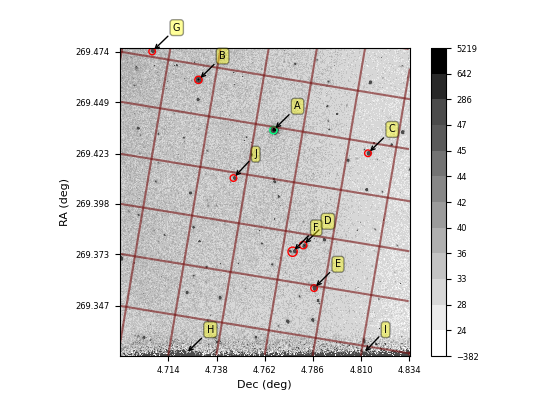
\includegraphics[scale=1]{images/initgexample.png}
\end{center}   
\caption{This is an observation of {\bstar} taken with the \texttt{g} filter on
17 September 2018 at 02:58:52 UTC after processing using the master bias and
flat files for September 2018. The brightest object, marked \textbf{A} and marked in
green is \bstar, whilst the next 9 brightest objects are marked in yellow and
\textbf{B}, \textbf{C}, etc. in decreasing order of brightness.}
\protect\label{fig:initgexample}
\end{figure}

\begin{figure}[!htbp]
\begin{center}
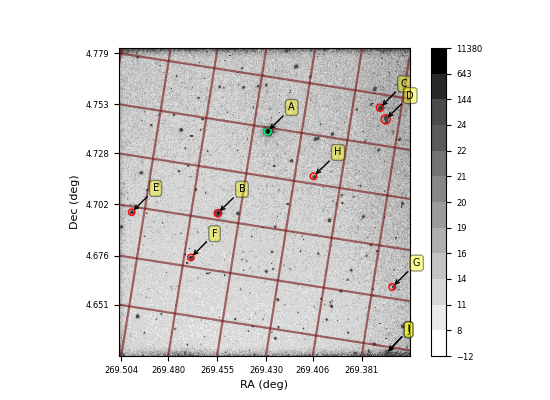
\includegraphics[scale=1]{images/initgexample20.png}
\end{center}   
\caption{This is an observation of {\bstar} taken with the \texttt{g} filter on
7 March 2020 at 09:07:23 UTC after processing using the master bias and
flat files for March 2020. The brightest object, marked \textbf{A} and marked in
green is \bstar, whilst the next 9 brightest objects are marked in yellow and
\textbf{B}, \textbf{C}, etc. in decreasing order of brightness.}
\protect\label{fig:initgexample20}
\end{figure}

In nearly every case there are 4 images taken, one with each of the 4 visible
light filters (in addition to the simultaneous REMIR observations) and in Fig.
\ref{fig:initgexample} is illustrated a set of observations of {\prox} taken on
the same date, 17 September 2018 as the observation of {\bstar} in Fig.
\ref{fig:initgexample}. For comparison, in Fig. \ref{fig:init4example20} is
shown a set of observations taken on 9 March 2020.

\begin{figure}[!htbp]
\begin{center}
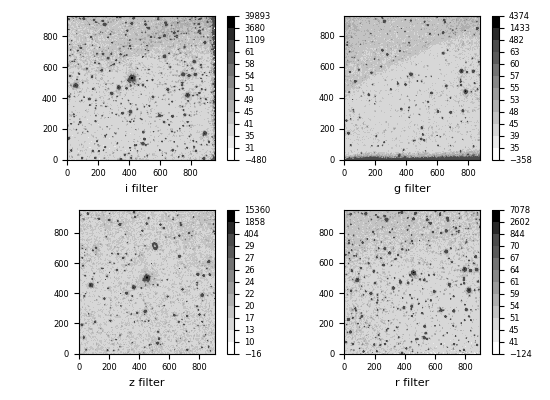
\includegraphics[scale=1]{images/init4example.png}
\end{center}   
\caption{This is all 4 observations of {\prox} taken with the visible light
filters on 17 September 2018 at 02:12:40 UTC after processing using
appropriate master bias and flat files for September 2018. They are arranged in
the order and orientation in which they are taken from the CCD. The
divisions on each image are pixel numbers.}
\protect\label{fig:init4example}
\end{figure}

\begin{figure}[!htbp]
\begin{center}
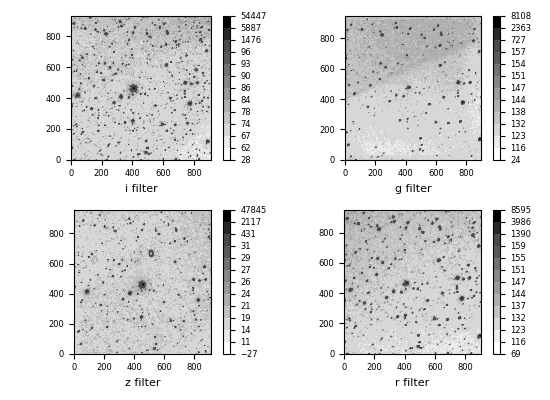
\includegraphics[scale=1]{images/init4example20.png}
\end{center}   
\caption{This is all 4 observations of {\prox} taken with the visible light
filters on 9 March 2020 at 08:56:14 UTC after processing using
appropriate master bias and flat files for March 2020. They are arranged in
the order and orientation in which they are taken from the CCD. The
divisions on each image are pixel numbers.}
\protect\label{fig:init4example20}
\end{figure}

\subsubsection{Some sample light curves}
\protect\label{section:samplelightcurves}

In Fig. \ref{fig:lcurvesing} is presented light curves of ADUs from {\prox}
from the observations on 16 and 17 September 2018 for the \texttt{g} and
\texttt{r} filters. In Fig. \ref{fig:lcurveref} is shown the same observations
where the ADUs are divided by the total ADUs of a subset of objects common to
all of the the other observations.

\begin{figure}[!htbp]
\begin{center}
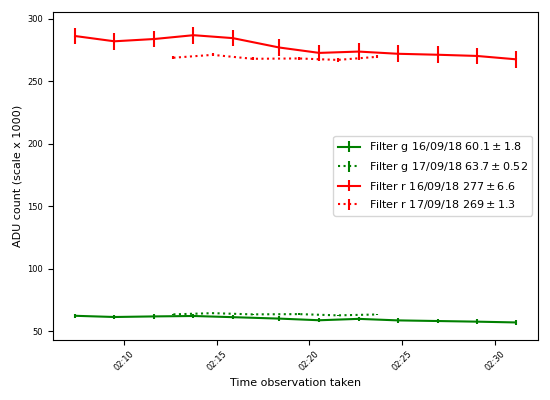
\includegraphics[scale=1]{images/demo_lcurve.png}
\end{center}   
\caption{This shows the total ADUs from the observations of {\prox} on 16 and
17 September 2018 for the \texttt{r} and \texttt{g} filters. The plot for each
day is overlaid to show the time taken.The results for those filters are in the appropriate colours
with the later date dotted.}
\protect\label{fig:lcurvesing}
\end{figure}

\begin{figure}[!htbp]
\begin{center}
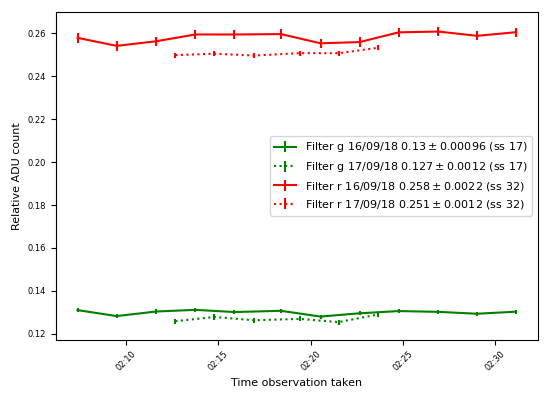
\includegraphics[scale=1]{images/demo_lcurve_refs.png}
\end{center}
\caption{This shows the total ADUs from the observations of {\prox} on 16 and
17 September 2018 for the \texttt{r} and \texttt{g} filters, (the same as in
Fig. \ref{fig:lcurvesing}) divided by the total of the ADUs for a subset of
other objects common to all the observations. The legend in each case shows the
subset size of the reference objects. }
\protect\label{fig:lcurveref}
\end{figure}

\clearpage

% \subsection{Point spread functions}
% \protect\label{section:pointspreadfunc}
% 
% In Fig. \ref{fig:im3d} is shown a 3D representation of the \texttt{g} filter
% observation of {\prox} shown in Fig. \ref{fig:init4example}.
% 
% \textit{I plan to zoom in on some of the objects showing the cross-section in
% various planes to illustrate that the objects are close to Gaussian in profile.
% I then show how I can optimise the aperture for the objects to give an
% acceptable accuracy across various frames. Also note that circular apertures
% are sufficient, sufficiently few would benefit from using an elliptical
% aperture to merit time being spent on these.}
% 
% \begin{figure}[!htbp]
% \begin{center}
% 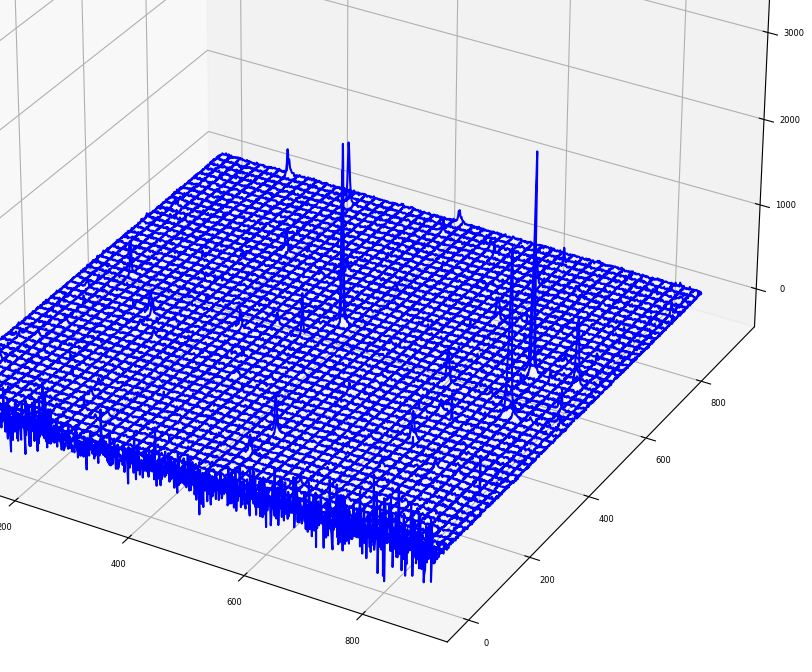
\includegraphics[scale=0.5]{images/im3d.png}
% \end{center}
% \caption{This is a 3-D representation of the \texttt{g} filter observation of
% {\prox} already shown in Fig. \ref{fig:init4example} illustrating the peaks of
% some of the objects.} \protect\label{fig:im3d}
% \end{figure}
% 
% \clearpage

\subsection{Matters addressed in analysing data}
\protect\label{section:mattersaddressed}

The results of the initial processing of the data as discussed above highlighted
the matters which should be addressed to accurately process the images.

\subsubsection{Uncertainty measure}
\protect\label{section:issueuncertainty}

The light curves shown in Fig. \ref{fig:lcurvesing} and Fig. \ref{fig:lcurveref}
have error bars shown according to the standard deviation of the ADU count and
the ratio to the reference stars respectively. Given that the observations are
taken over an initial period of at most 20 minutes, it is unsurprising that
these do not vary much. Part of the variations which are shown may be due to
varying noise in the pixels on the CCD which are different for each exposure.

However the observations are all using the same master flat and bias files. It
is not clear what the uncertainty is on those files, so some analysis is
necessary.

\subsubsection{Flat files}
\protect\label{section:issueflatfiles}

It is of concern that there is a shading towards the bottom of the image; this
is the \texttt{g} filter, for which the bottom part of the image is taken from
the central part of the CCD (the \texttt{g} filter image is taken from the
upper right portion of the CCD, with the origin close to the centre of the CCD).
In Fig. \ref{fig:init4example} is the set of all visible light observations of
\prox, taken on the same date as in Fig. \ref{fig:initgexample} of 17 September 2018 at
02:12:40 UTC, with the images displayed in the sequence in which they are taken
from the CCD. For comparison, the same observations, without application of the
flat fields (but still with subtraction of the bias fields), are presented in
Fig. \ref{fig:init4exnoflat}. Also for comparison, in Fig.
\ref{fig:init4example20}, are observations of {\prox} parallel to those in Fig.
\ref{fig:init4example} from March 2020.

\begin{figure}[!htbp]
\begin{center}
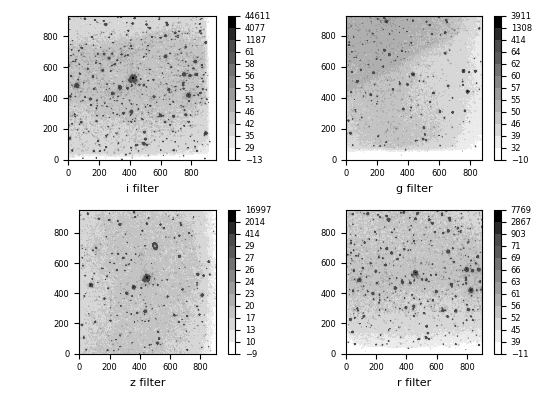
\includegraphics[scale=1]{images/init4exnoflat.png}
\end{center}   
\caption{This is all 4 observations of {\prox} taken with the visible light
filters on 17 September 2018 at 02:12:40 UTC, the same as in Fig.
\ref{fig:init4example}, after processing using appropriate master bias but
omitting the flat files for September 2018. The divisions on each image are pixel numbers.}
\protect\label{fig:init4exnoflat}
\end{figure}

It can be seen that the shading at the sides of the images is introduced by
applying the master flat fields.

\subsubsection{Negative pixels}
\protect\label{section:issuenegpixels}

Of additional concern is that a number of the pixel values are
negative after subtracting the bias value for each pixel. This in some cases is
larger than the pixel value at the same location in the observation file.
It would be expected that the bias level, with exposure of zero, should be
everywhere lower than any pixel observing sky, but this is not the case. For the images shown in Fig.
\ref{fig:init4example} the number of negative pixels are as shown in Table
\ref{table:initexnegpix}.

\begin{table}[!htbp]
\begin{center}
\begin{tabular}{lrrr} \hline
Filter & No of pixels & No negative & \% \\\hline
g & 818,296 & 763 & 0.09 \\
r & 858,600 & 388 & 0.05 \\
i & 898,560 & 2,143 & 0.24 \\
z & 866,136 & 1,401 & 0.16 \\
Total & 3,441,592 & 4,695 & 0.14 \\

\hline
\end{tabular}
\end{center}
\caption{Negative pixels in the images shown in Fig. \ref{fig:init4example} for
the various filters.}.
\protect\label{table:initexnegpix}
\end{table}

\subsubsection{Other caveats}
\protect\label{section:otherissues}

Of some concern is the ring shaped artefact above and slightly to the right of
the brightest objects in the images for the \texttt{z} filter, invariably for
the target, but to a greater or lesser degree for the other objects. Often the
artefact lands entirely on another object, compromising the usability of the
frame.

The \texttt{z} filter is poorest in terms of other objects in the frame for all
of the objects and there are few objects to be found in common subsets across
all the frame, this being because, despite being classified as ``visible
light'', it is in the near Infrared and the {\rdwarf} targets are much brighter
in this band then the other objects.

As a result, it proved advisable to avoid the \texttt{z} filter as it would not
be practical to try to compensate for the artefact given the likely poor return
if this were done. In any case the this is often worst or next to worst in terms
of the number of the negative pixels are to be found in the observations from
this filter, as shown in Table \ref{table:initexnegpix}.

\clearpage

\section{Analysis of calibration files}
\protect\label{section:analysiscalib}

\textit{I wonder if this section should be considerably condensed at it doen't
contribute too much except to show all the blind alleys I've been up, the later
work on bad pixels is much more promising for eliminating the bulk of the
negative pixels and I can use more of the daily flats. I think I need to
explain why I think the master bias and flat files don't cut it and the efforts
made to replace them and also keep track of the error bars on them.}

The initial display of images and preliminary results shown above raise
questions about the calibration files used, so some effort was undertaken to
study these and perhaps make adjustments.

\subsection{Analysis of bias files}
\protect\label{section:biasanal}

Two sample sets of master bias files are illustrated in Fig. \ref{fig:mastbeg0918} and Fig.
\ref{fig:mastbeg0120}, either side of the change to the areas and starting
positions on the CCD in March 2019.

\begin{figure}[!htbp]
\begin{center}
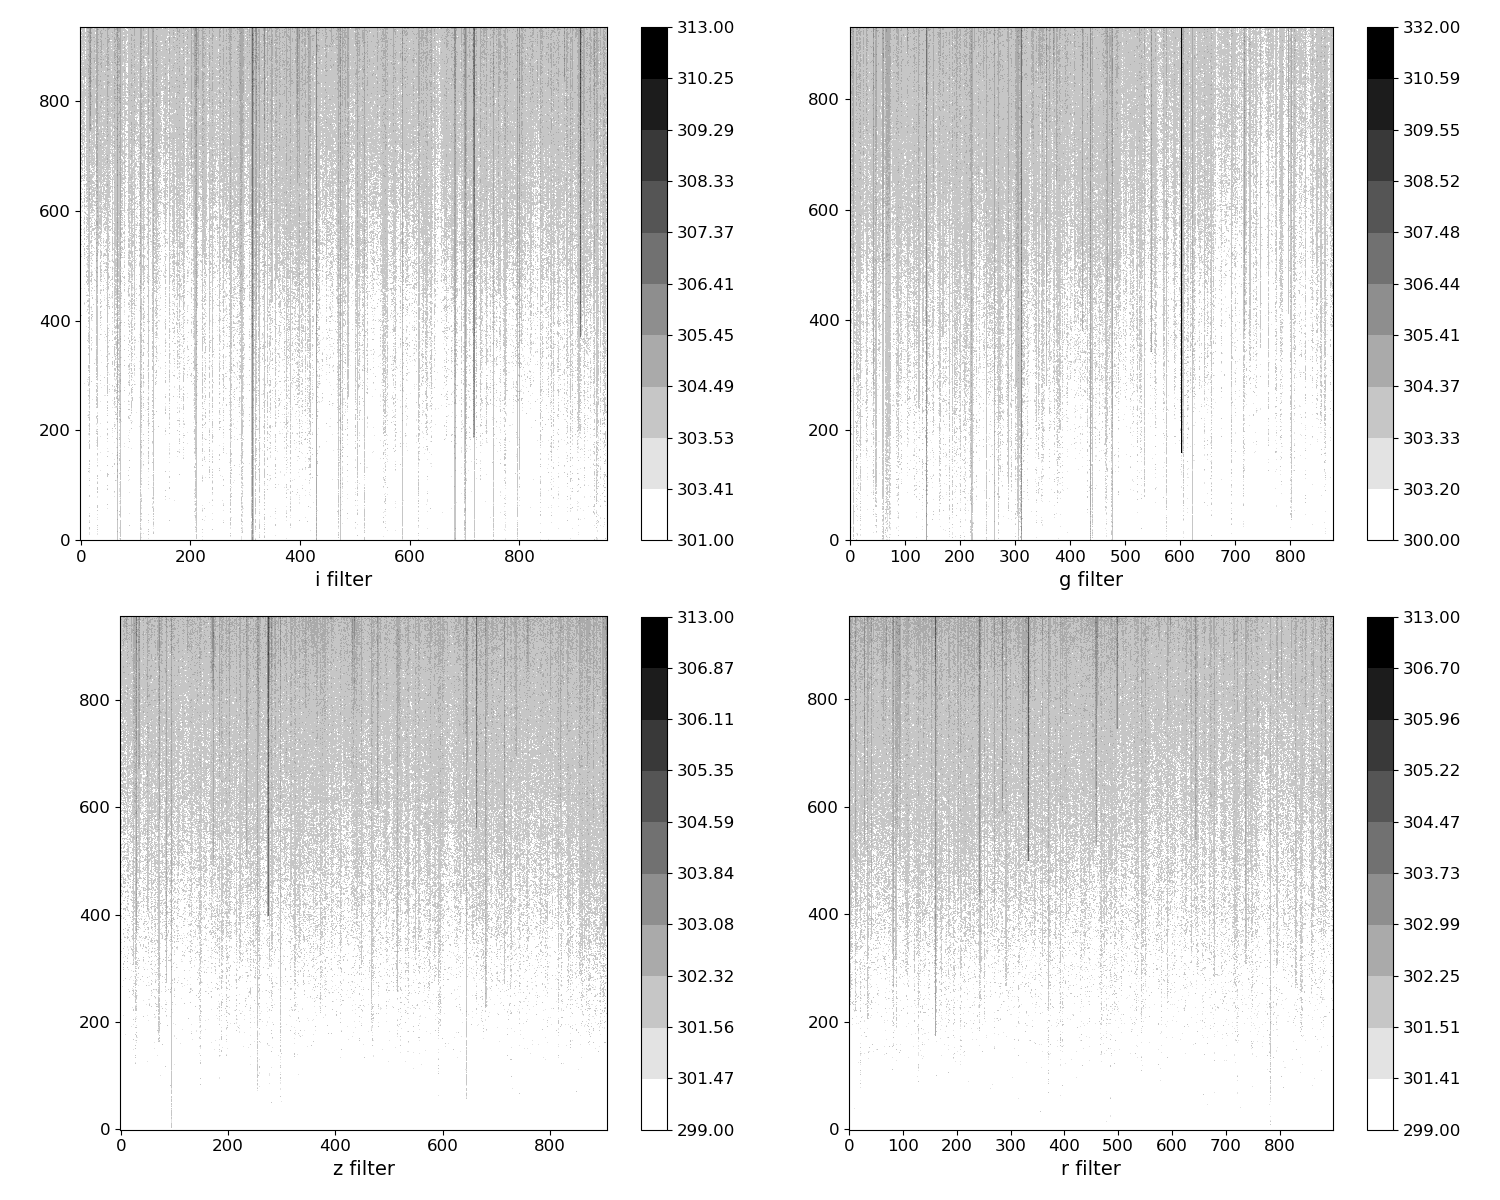
\includegraphics[scale=0.4]{images/mastbiaseg0918.png}
\end{center}   
\caption{This illustrates the 4 master bias files (provided for September
2018) for each filter used to construct Fig. \ref{fig:initgexample} and Fig.
\ref{fig:init4example}. The positions of the 4 images reflect the positions and orientations in which the
images are taken from the CCD.}
\protect\label{fig:mastbeg0918}
\end{figure}

\begin{figure}[!htbp]
\begin{center}
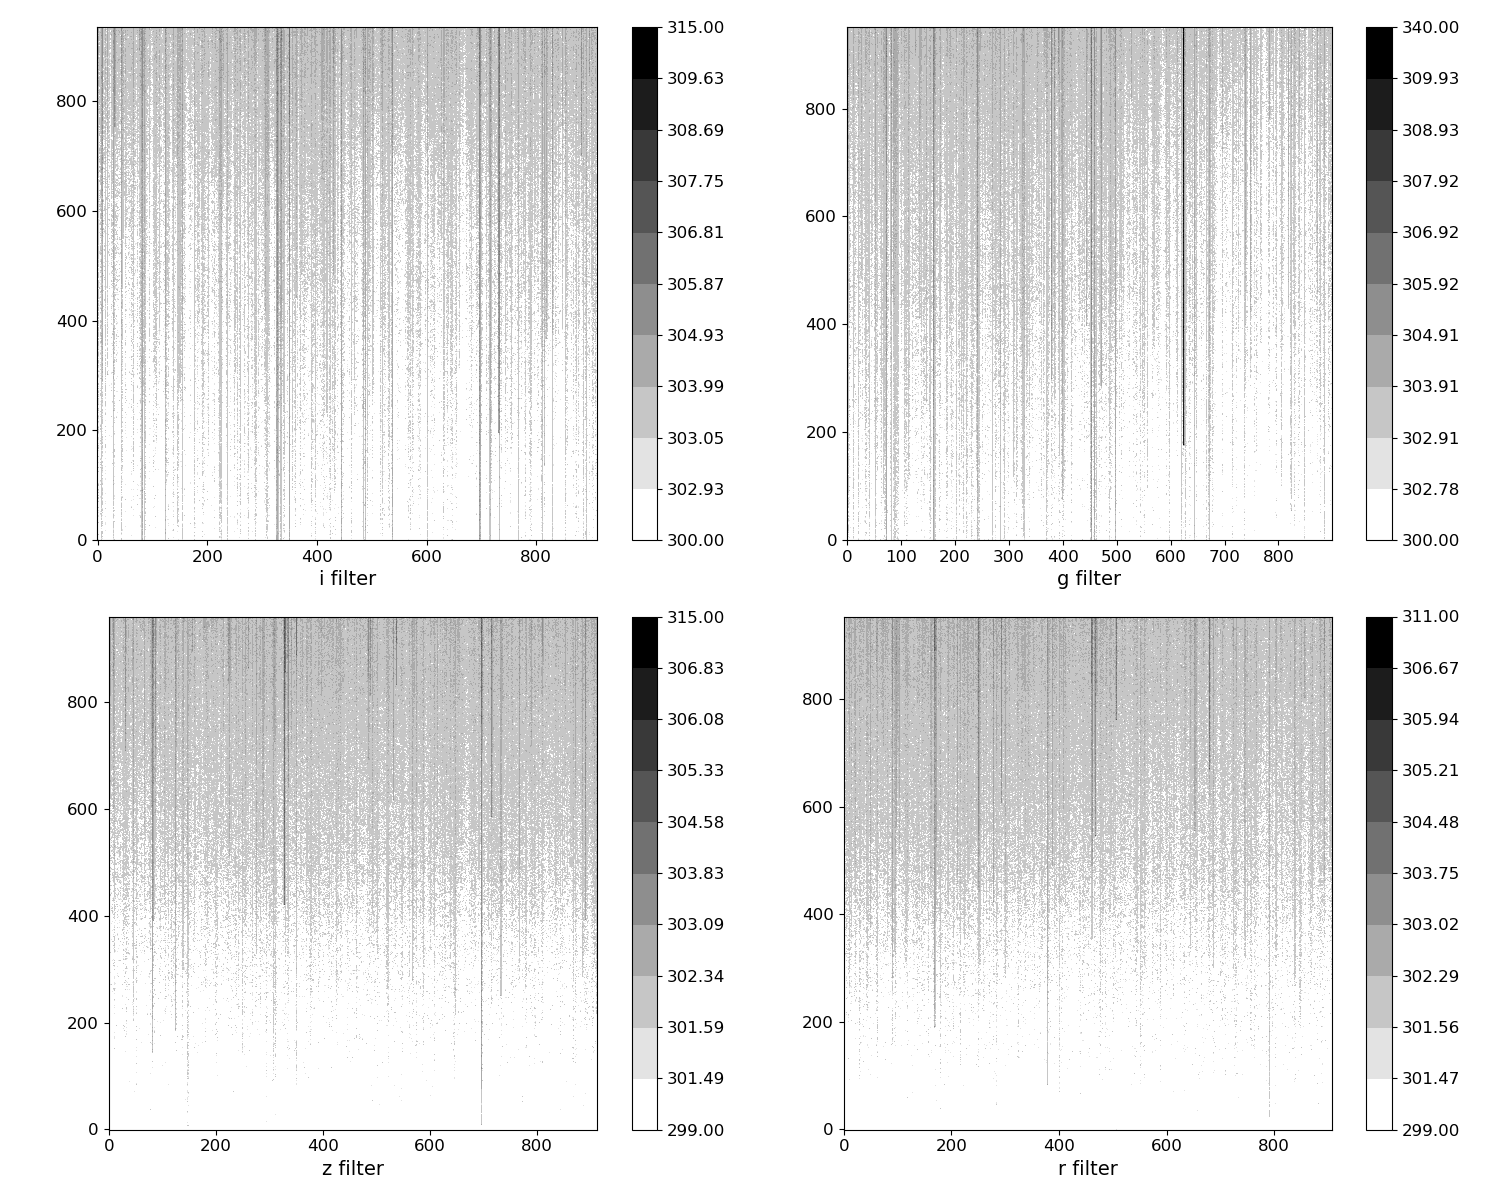
\includegraphics[scale=0.4]{images/mastbiaseg0120.png}
\end{center}   
\caption{This illustrates the 4 master bias files for each filter for January
2020, for comparison with Fig. \ref{fig:mastbeg0918}. The differences are due
to changes in the area and starting positions on the CCD for images made in
March 2019.}
\protect\label{fig:mastbeg0120}
\end{figure}

A study was made of the bias files to ascertain the level of the bias current
and assess the noise. Of particular concern was that subtraction of the bias
from observation files, in all cases, not just the most noisy bias files, yielded
negative pixel results from all the observation files, particularly those from
the \texttt{g} and \texttt{z} filters, for example, taking the
observations and master bias files for 5  September 2018, the total negative values shown in 
Table \ref{table:negmast} are observed.

\begin{table}[!htbp]
\begin{center}
\begin{tabular}{lrr} \hline
Filter & Min & \% negative \\\hline
g & -27 & 28.90 \\
i & -20 & 5.42 \\
r & -19 & 5.52 \\
z & -20 & 9.90 \\
\hline
\end{tabular}
\end{center}
\caption{Negative values of pixels in image minus monthly master bias for
various filters on 5 September 2018, for all observations of \bstar, through
various visible light filters}.
\protect\label{table:negmast}
\end{table}

This was also found in the daily flat files, although it proved possible to
eliminate them by careful choice of the daily  flat files as described in
Section \ref{seciion:altmasters}.

The location of the negative pixels is distributed quite widely across the
images, there is no restriction to a handful of places which could be identified
as bad pixels and made into a mask. This can be demonstrated by examining
observation files, subtracting the relevant master bias file for the month and
counting where each pixel goes negative. The result can be seen in Fig.
\ref{fig:negpixloc}. It will be clear that pixels can become negative all over
the images, but the edges of the images from some of the filters, for example
the bottom edge of the \texttt{g} filter and the right edge of the \texttt{z}
filter are especially bad.

\begin{figure}[!htbp]
\begin{center}
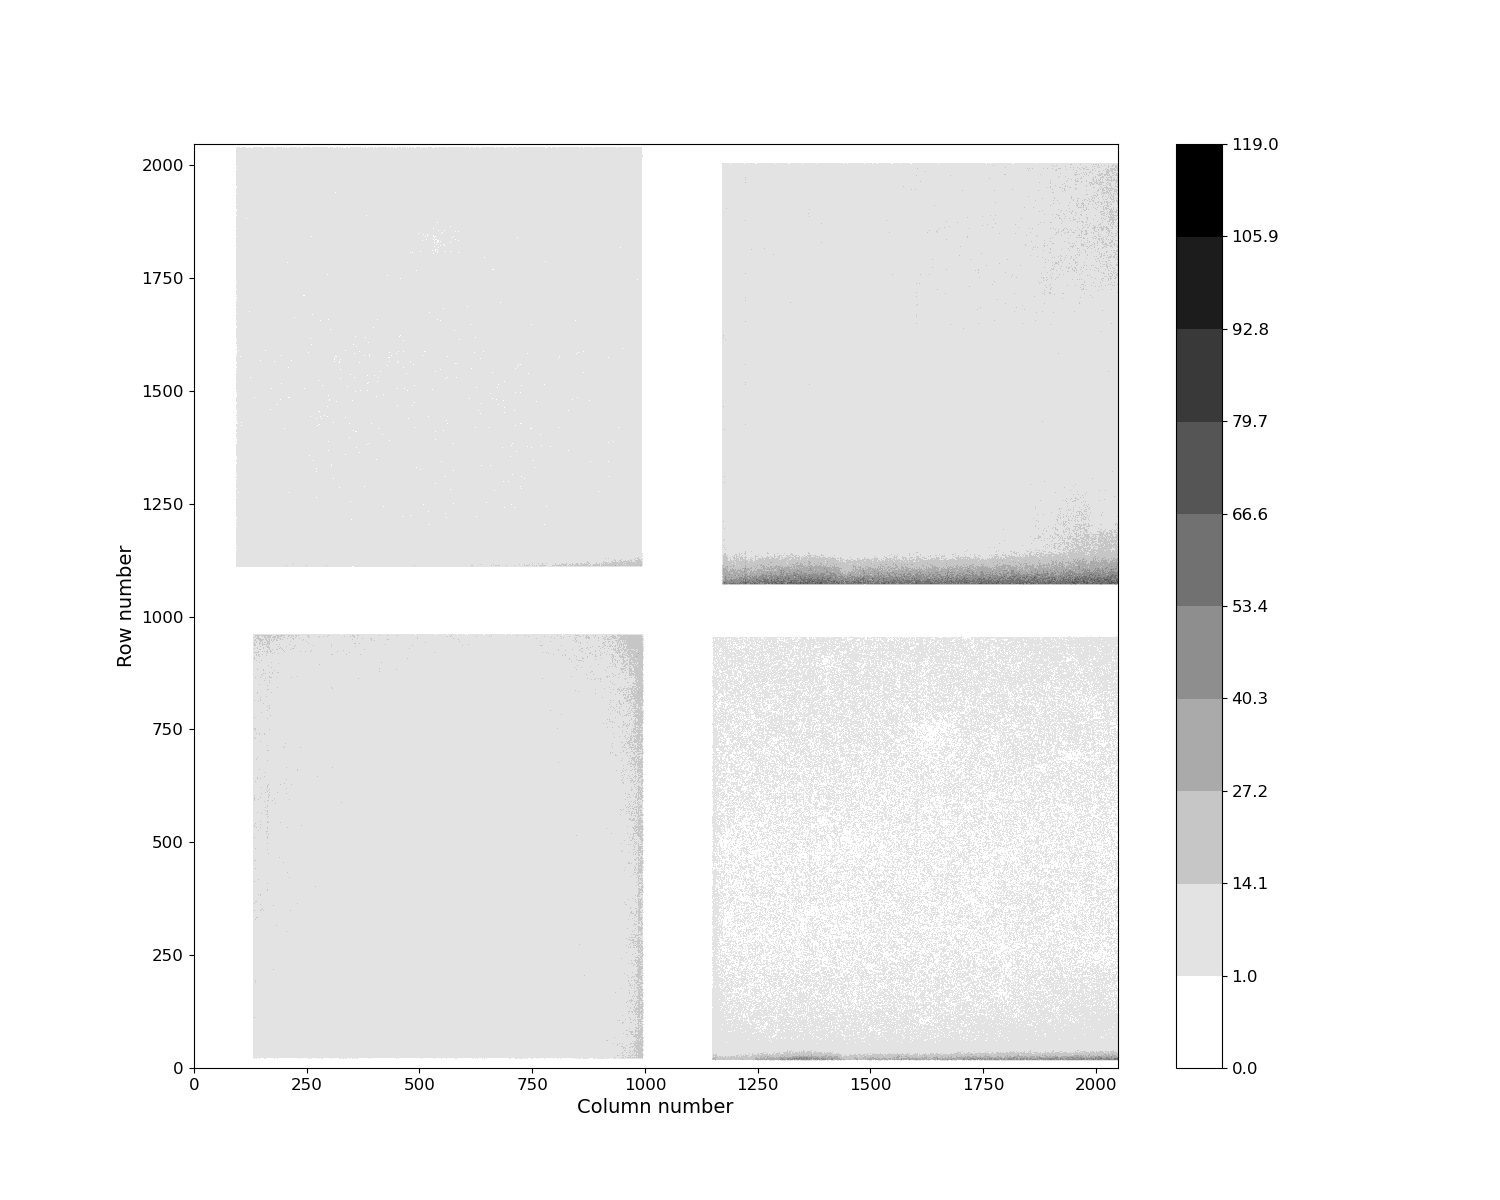
\includegraphics[scale=0.4]{images/min200negpix.png}
\end{center}   
\caption{This shows a representation of the entire CCD array and
analysing all the observations (omitting those with minimum values less than
200 counts or greater than 61,000 counts in one or more pixels) for each of the
visible light filters, counting each time the corresponding pixel goes negative
after subtraction the corresponding bias files. It may be helpful to compare this with Fig.
\ref{fig:showusedccd} to show the portions of the CCD used.}
\protect\label{fig:negpixloc}
\end{figure}

\subsubsection{Master bias files}
\protect\label{section:masterbiasfiles}

In Fig. \ref{fig:mastmeanbias} is shown the mean value and standard deviation of
the master bias files up to March 2020.

\begin{figure}[!htbp]
\begin{center}
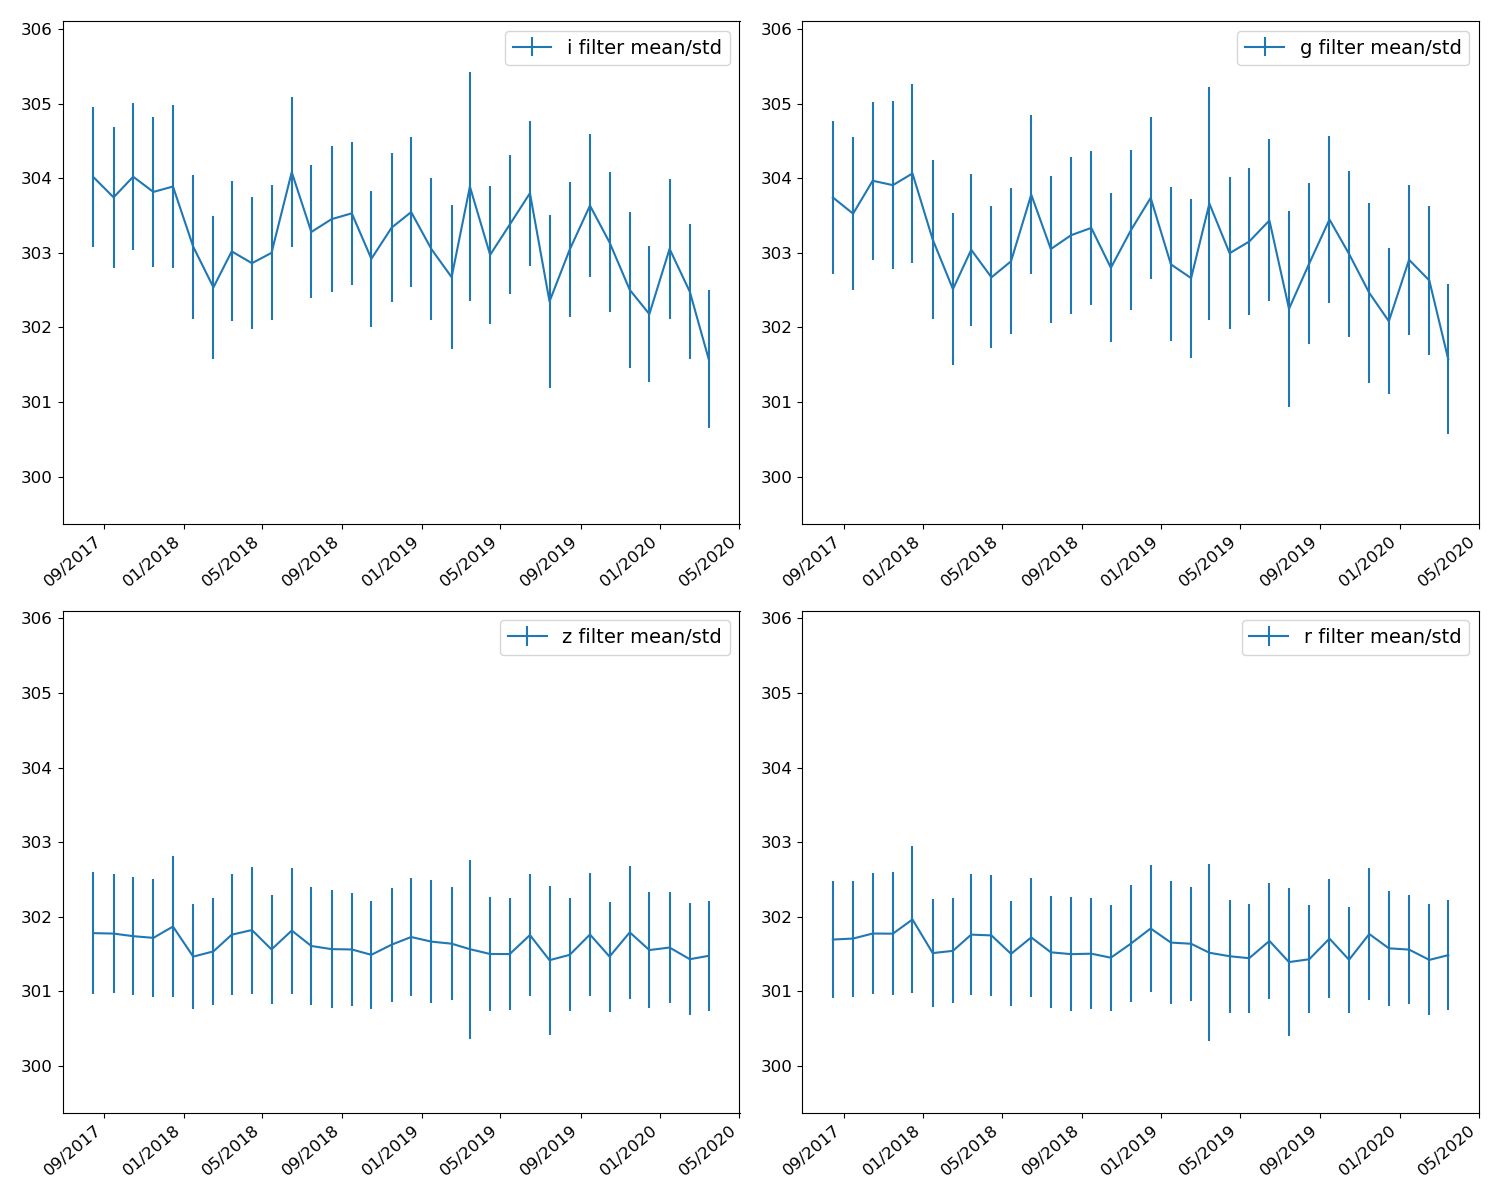
\includegraphics[scale=0.4]{images/mastmeanbias.png}
\end{center}   
\caption{This illustrates the mean and the standard deviation of the values in
the master bias files from July 2017, when {\rdwarf} targets were first
observed, until March 2020.}
\protect\label{fig:mastmeanbias}
\end{figure}
\clearpage

The master bias files are constructed from the daily bias files for the
corresponding month for each filter as follows:

\begin{enumerate}
  \item Tabulate the mean and standard deviation of each pixel count in each
  bias file.
  \item Take the median mean (\textit{med\_e}) and the median standard deviation
  (\textit{sd\_e}) of those.
  \item Take the daily bias files whose mean in less than 3 times \textit{sd\_e}
  deviations away from \textit{med\_e}.
\end{enumerate}

A study of the daily bias was made to investigate the construction of the master
bias files and determine whether adjustments would be valuable. It did appear at
first sight that the above procedure might play down the noise level of some of
the daily bias frames causing monthly bias files to differ unacceptably.

\subsubsection{Daily bias files}
\protect\label{section:dailybiasfiles}

A variety of examinations on the daily bias files were undertaken in order to
establish the noise levels of the pixels, the validity of the master bias files
and also to look for any bad pixels and pixels of more limited reliability.

As a first exercise, each of the daily bias files for one date was examined
against each other and the differences tabulated. The result can be seen in Fig.
\ref{fig:biasdiffs}. Various other dates were considered with very similar
results. Comparison over wider sets of dates did not alter the picture in any
significant way, the bias files do not differ particularly over the period.

\begin{figure}[!htbp]
\begin{center}
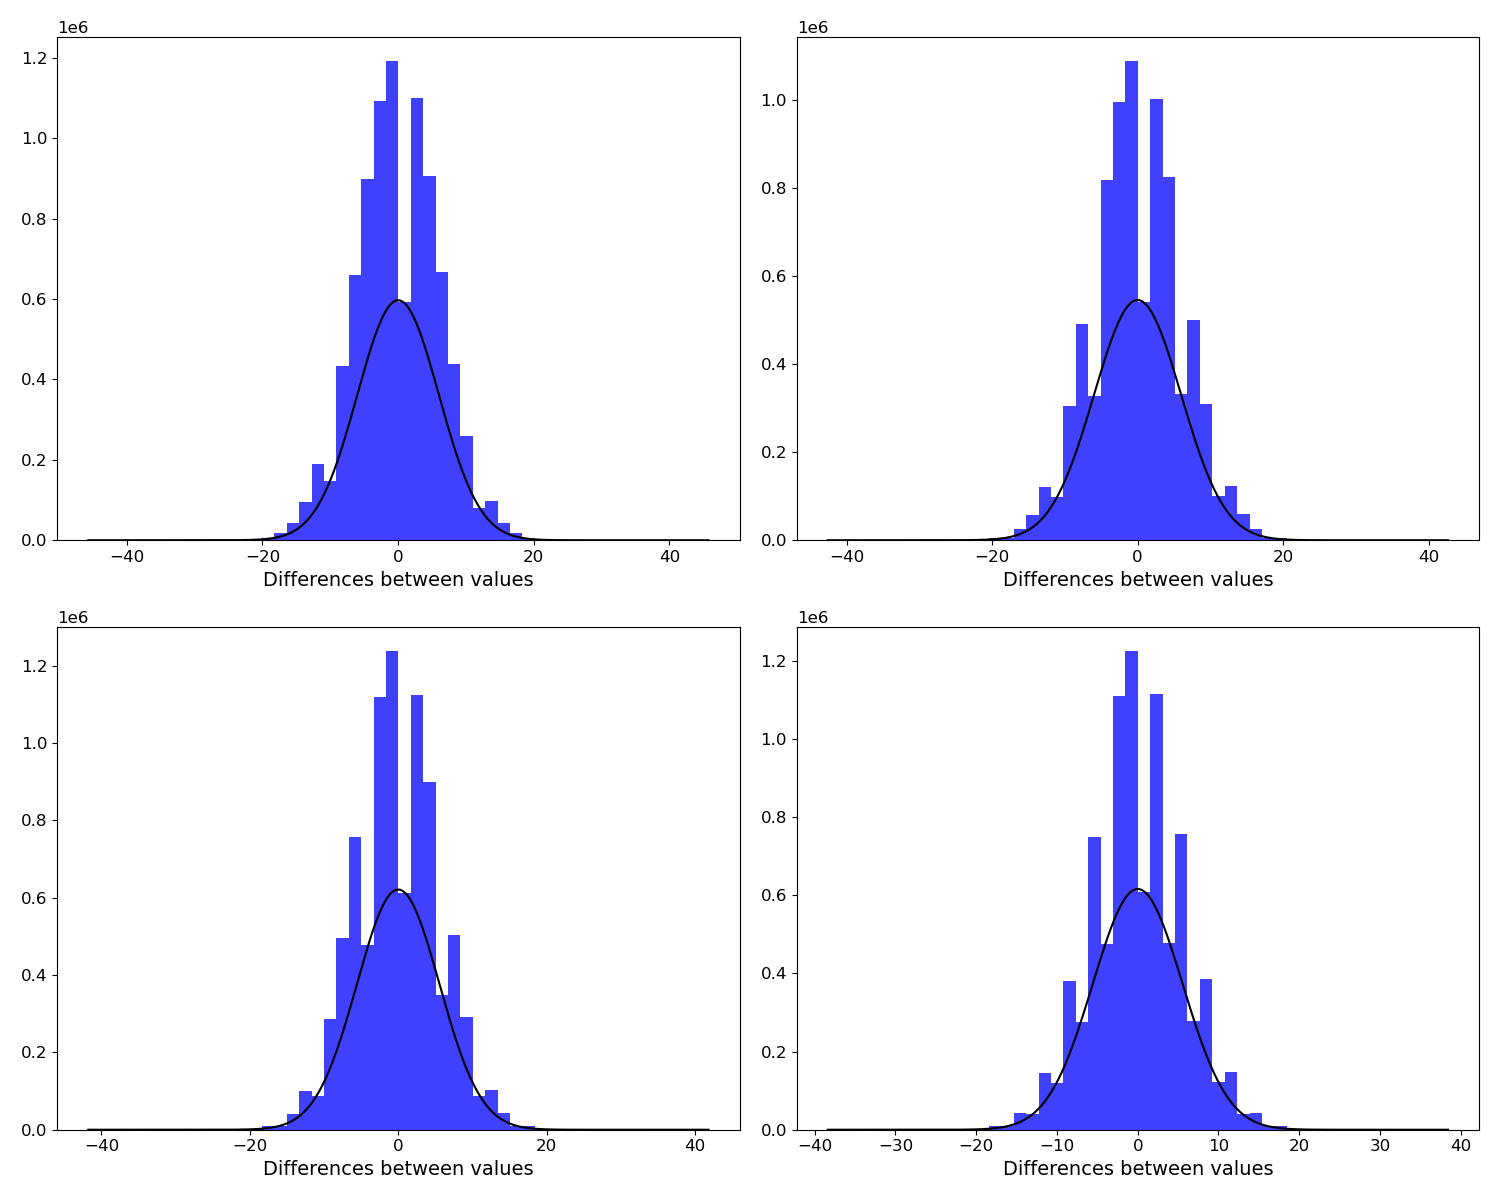
\includegraphics[scale=0.4]{images/biasdiffs.png}
\end{center}   
\caption{This image was constructed by taking all the daily bias files of 17
October 2018, 5 for each of the 4 visible light filters, and noting the
difference between the counts for each pixel between each file and each other
file. A Gaussian fitted to the same mean and standard deviation is overlaid.
In the histograms the very small number of outlying points above 6 standard
deviations is included in the outlying bins. The date was chosen at random, no
other date gave particularly different results.} \protect\label{fig:biasdiffs}
\end{figure}

\subsubsection{Construction of master bias files}
\protect\label{section:mastbiasconstr}

It was of possible concern that the method for constructing the master bias
files set out in Section \ref{section:masterbiasfiles} may include noisy bias
files but whose means are nevertheless within the selected range. By looking at
Fig. \ref{fig:mastmeanbias} a number of places were noted where the plot appears
to wander sharply. In \ref{fig:ibiasnolim} is illustrated the daily bias files
over a period where the master bias files differ quite sharply from month to
month. It is notable that there are some daily bias files with high noise but
also where the mean is close to the overall mean and thus would be included in
the construction of the master bias file. The number of daily bias files over
parts of these periods appears to be limited, with gaps of nearly 2 weeks in
some cases. The corresponding master bias files would appear to be less
reliable in these cases.

By excluding daily bias files with standard deviations less than 3 times the
standard deviation of standard deviations, the spread of daily bias files over
the same period takes the form seen in Fig. \ref{fig:bias3std} is seen. Again
days when no bias files are made as apparent.

\begin{figure}[!htbp]
\begin{center}
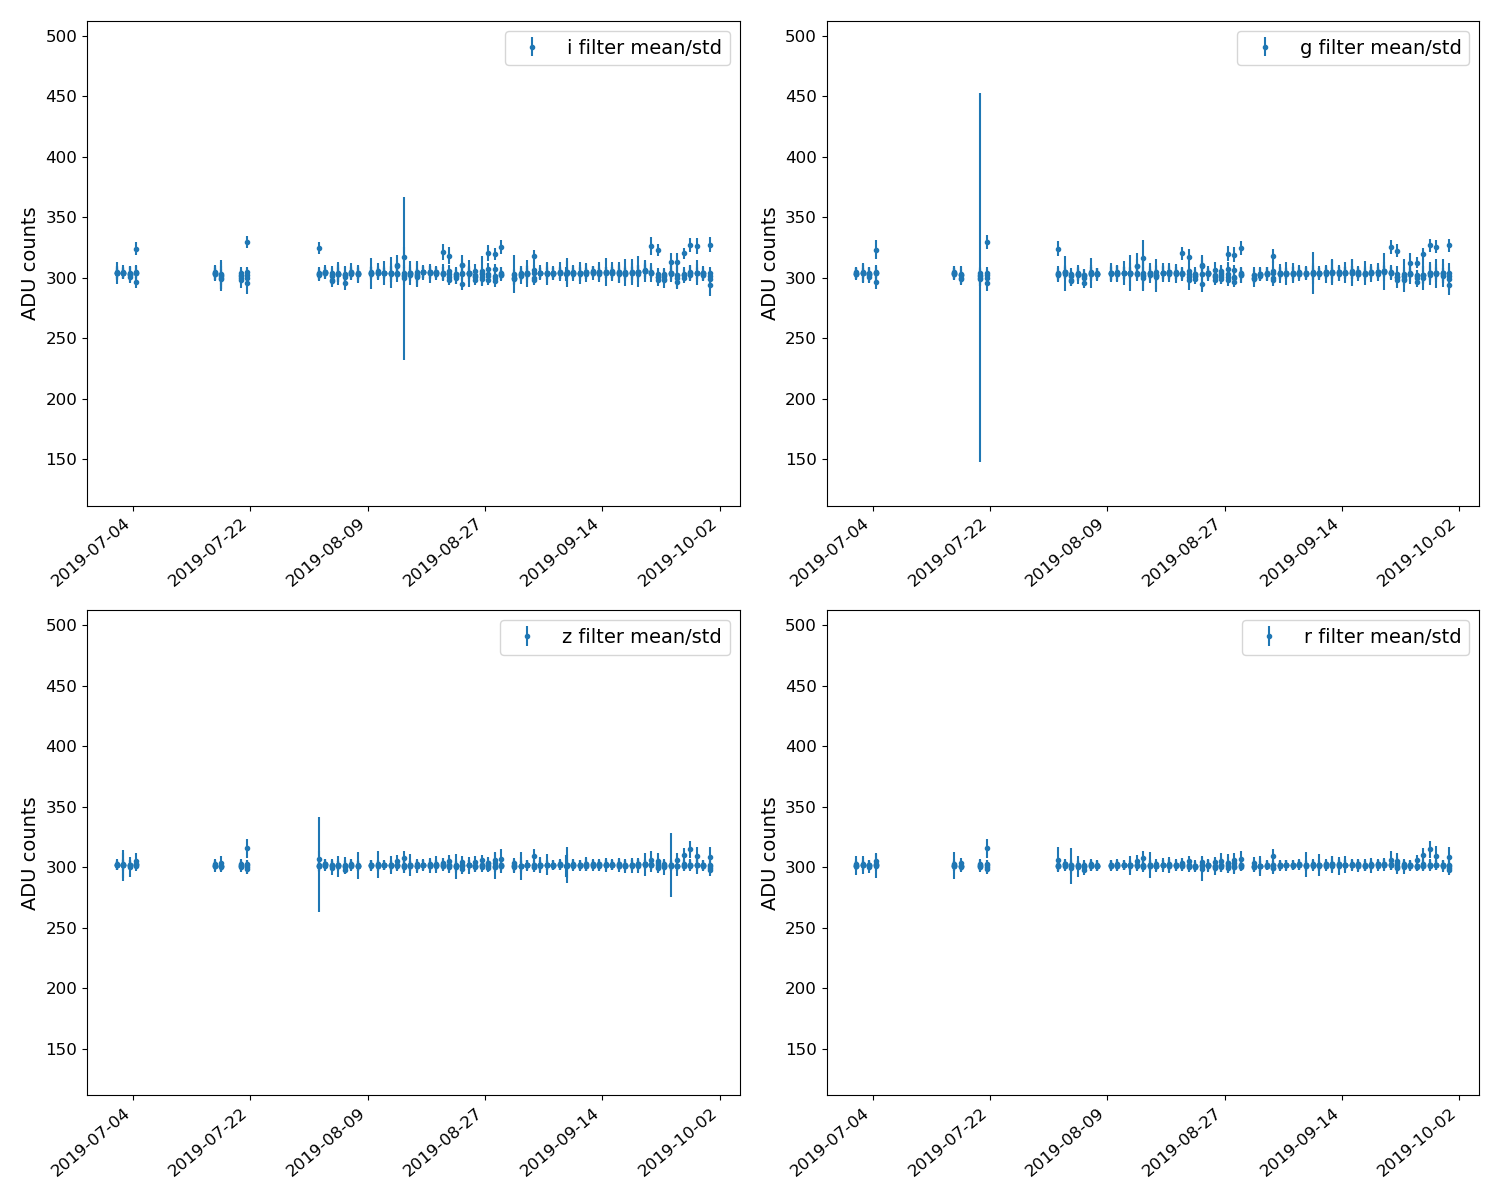
\includegraphics[scale=0.4]{images/ibiasnolim.png}
\end{center}   
\caption{This figure displays the daily bias files over the period July to
September 2019 inclusive showing the means and standard deviations for each
file. This corresponds to a section of Fig. \ref{fig:mastmeanbias} where
the variability is greater.} \protect\label{fig:ibiasnolim}
\end{figure}

\begin{figure}[!htbp]
\begin{center}
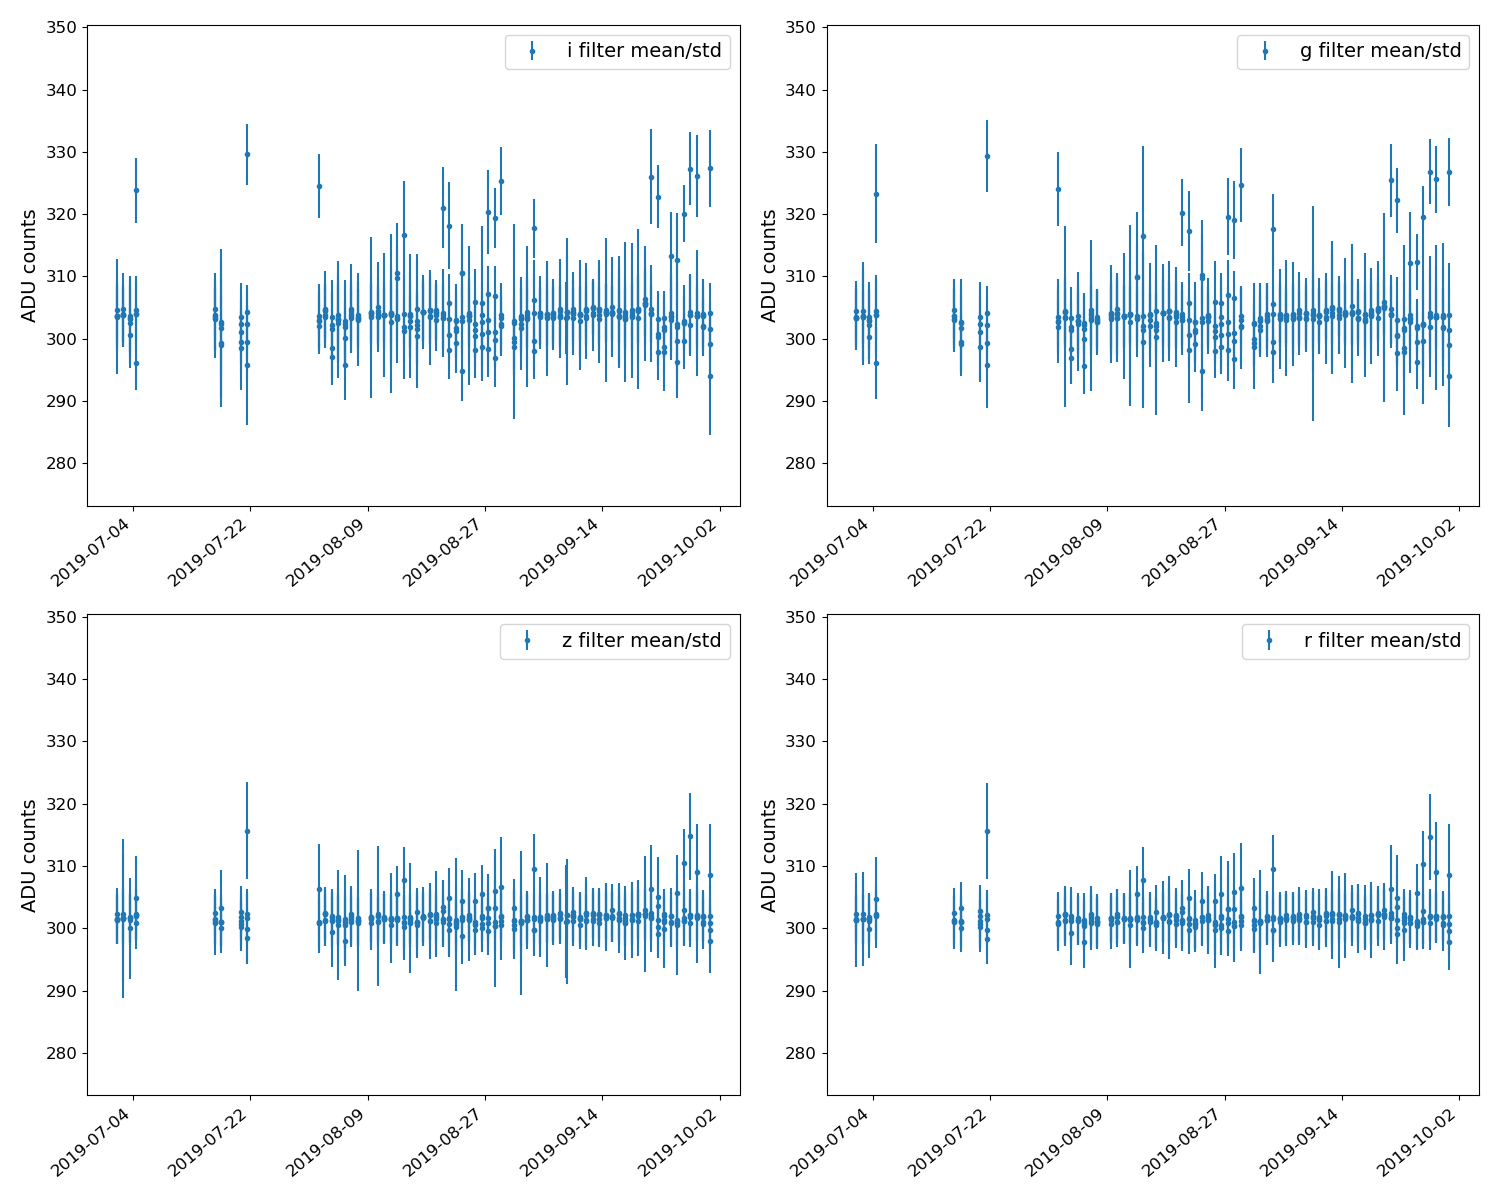
\includegraphics[scale=0.4]{images/ibiaslim3std.png}
\end{center}   
\caption{This figure shows the same daily bias files over the period July
to September 2019 as Fig. \ref{fig:ibiasnolim} but excluding the files whose
standard deviations from the means are greater than 3 times the standard
deviation of standard deviation of the overall standard deviations. Note that
the Y axis has a considerably narrower scale than in Fig. \ref{fig:ibiasnolim}.}
\protect\label{fig:bias3std}
\end{figure}

It would appear from this analysis that the master bias files constructed from
those over the month are not likely to be reliable as they are based upon too
few daily bias files and some of the files included in the construction of the
master bias files are particularly noisy. \textit{I'm going to put in a short study showing
progression of bias levels and noise over time here.}

The conclusion from this study is to replace the master bias files with a
``rolling'' master bias files constructed from a window of bias files with, as
far as possible, the same number of daily bias files either side. It should be
noted that the processing of the most recent observational images will have to
be redone later to take into account later daily bias files giving a window
symmetric about the observation dates. This is not expected to make a
large difference, but for completeness, it is done.

As the noise on each pixel varies considerably, rather than having an overall
value for the standard deviation of the constructed master bias file, it costs
little in terms of additional resources to calculate and use a separate standard
deviation value for each pixel.

\clearpage

\subsection{Analysis of flat files}
\protect\label{section:flatanal}

The images displayed in the previous sections utilised the master flat files for
the appropriate month (in addition to the master bias files). First these files
were considered, before turning to the daily flat files, from which these are
constructed.

\subsubsection{Master flat files}
\protect\label{section:mastflats}

The image in Fig. \ref{fig:initgexample} and the images in Fig.
\ref{fig:init4example} were processed using the master flat and bias files for
September 2018. In Fig. \ref{fig:mastfeg0918} is illustrated the master flat
file for each filter. (The master bias file for each filter is shown in Fig.
\ref{fig:mastbeg0918} and discussed in Section \ref{section:biasanal}.) For
comparison, the master flat file for January 2020 is shown in Fig.
\ref{fig:mastfeg0120}. (The master bias file for January 2020 is shown in Fig.
\ref{fig:mastbeg0120} in Section \ref{section:biasanal}.) The reason for
including this latter image is that the telescope configuration was changed
slightly in March 2019.

\begin{figure}[!htbp]
\begin{center}
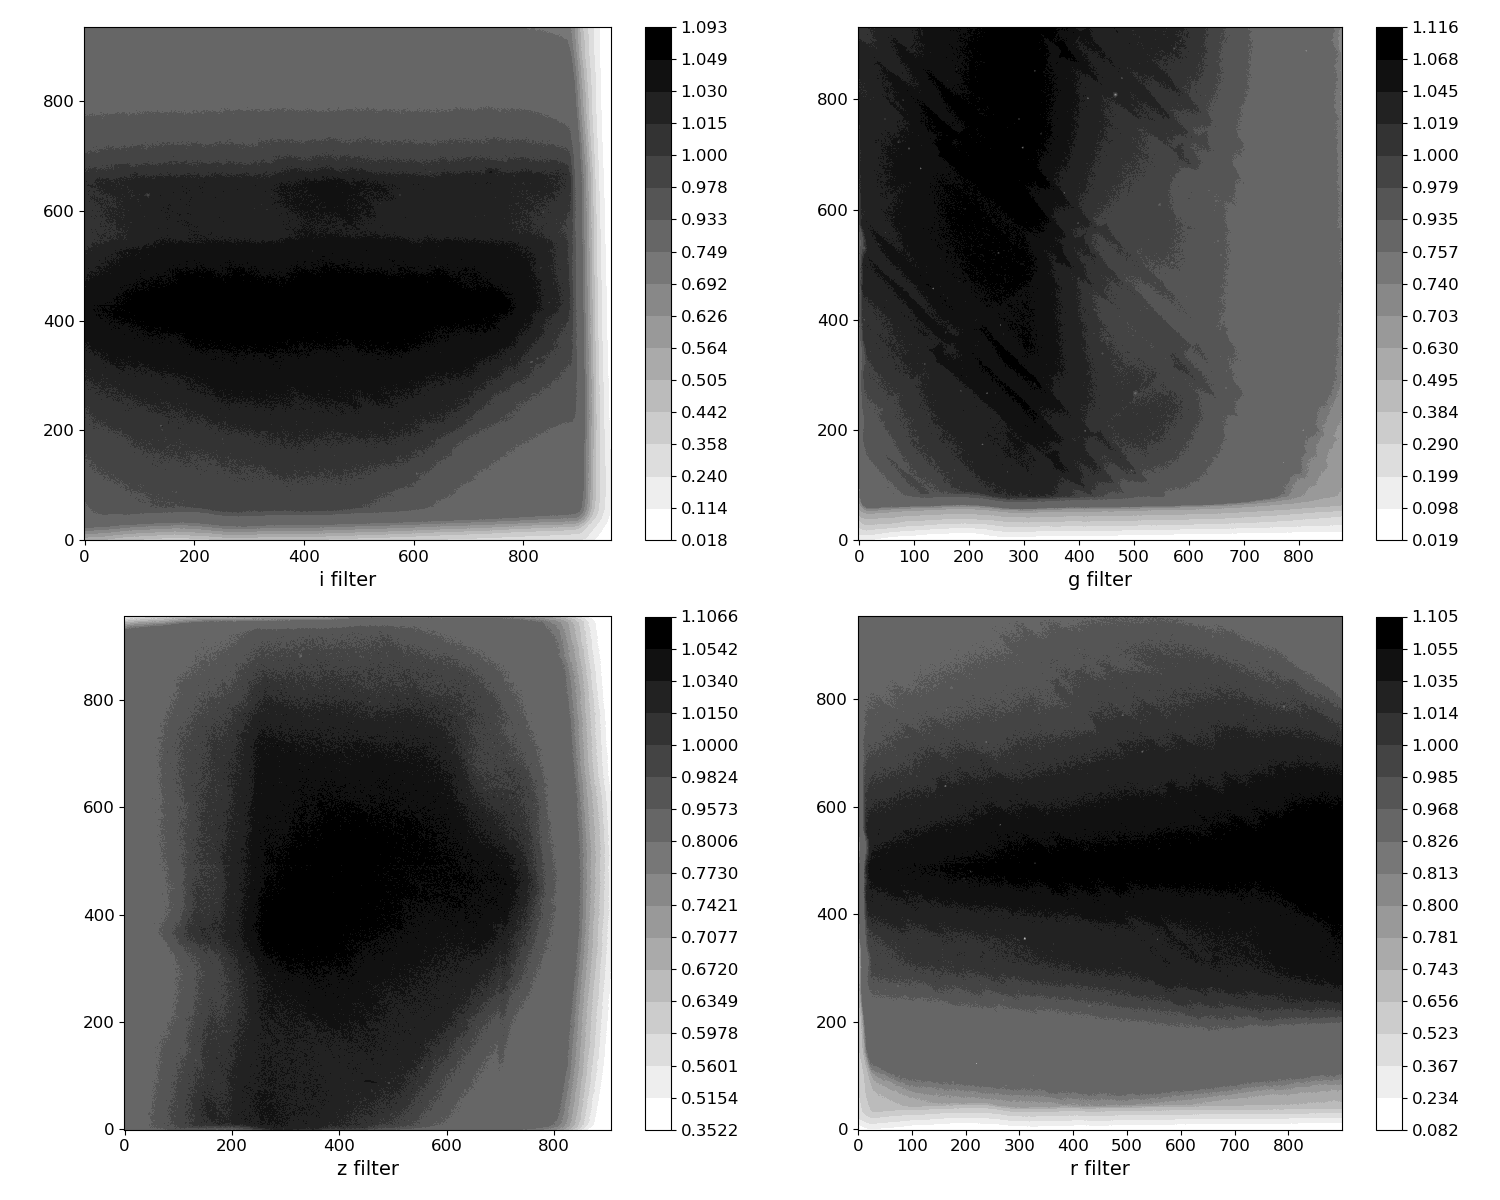
\includegraphics[scale=0.4]{images/mastflateg0918.png}
\end{center}   
\caption{This illustrates the 4 master flat files for each filter used to
construct Fig. \ref{fig:initgexample} and Fig. \ref{fig:init4example}. The
positions of the 4 images reflect the positions and orientations in which the
images are taken from the CCD.}
\protect\label{fig:mastfeg0918}
\end{figure}

\begin{figure}[!htbp]
\begin{center}
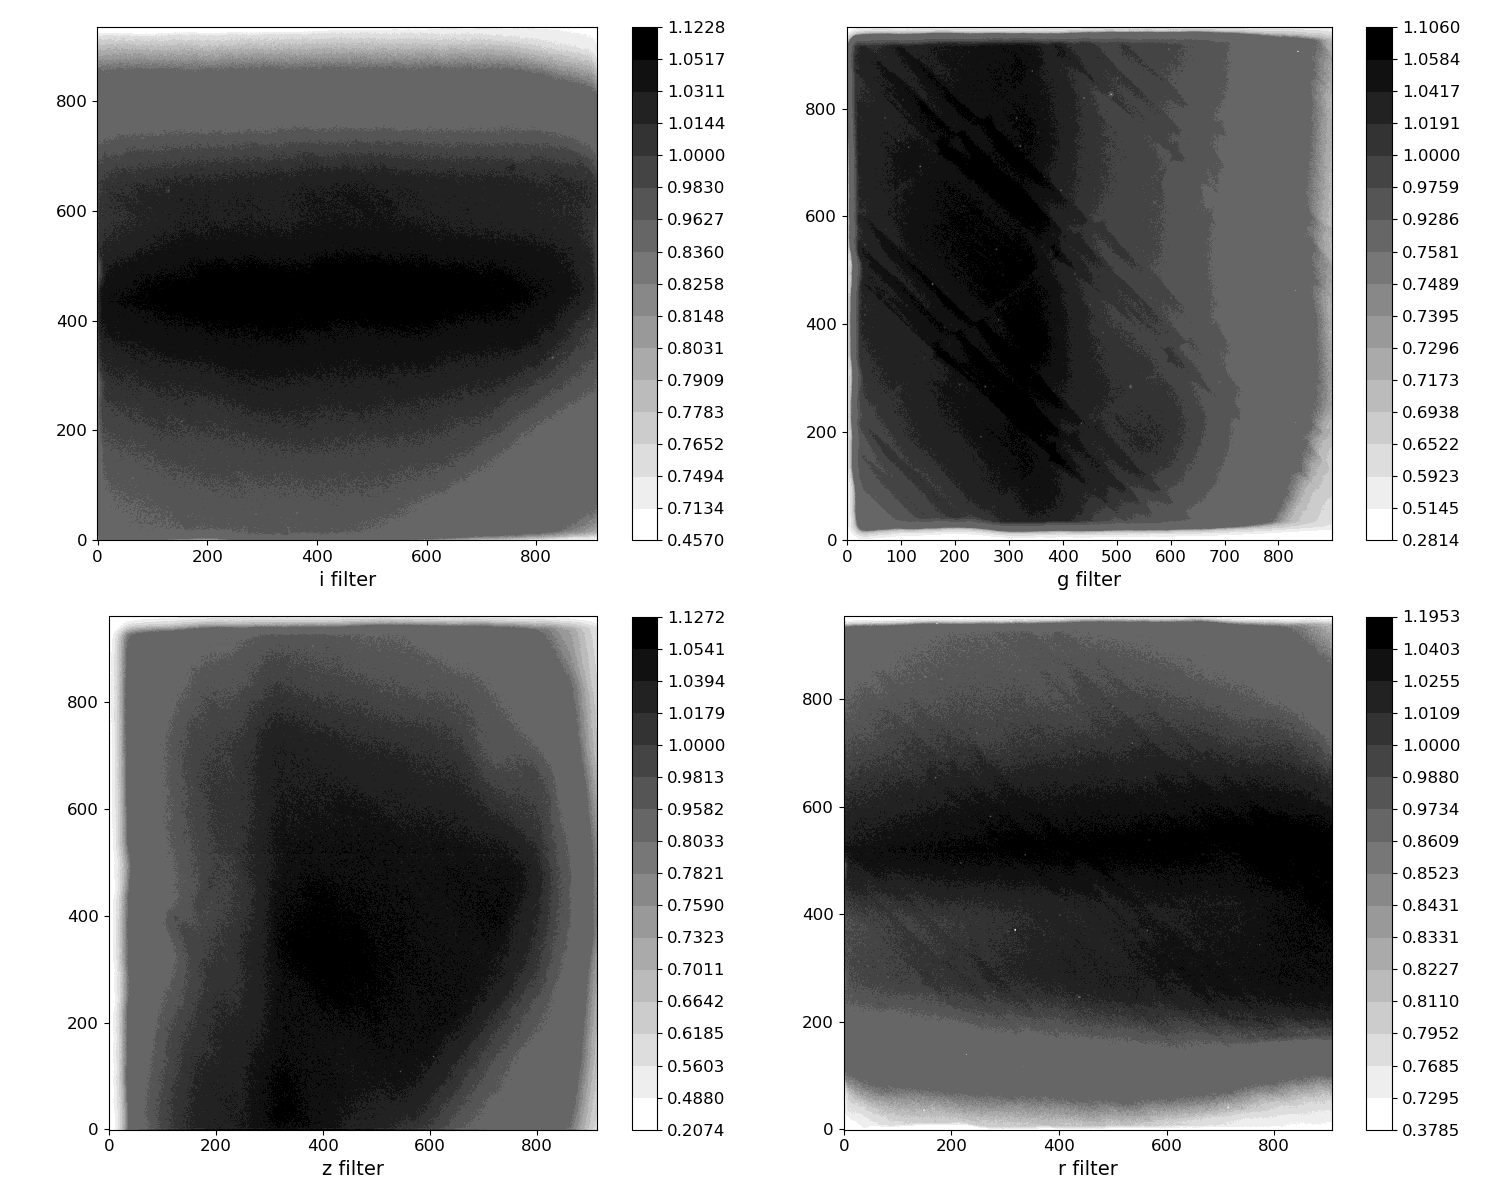
\includegraphics[scale=0.4]{images/mastflateg0120.png}
\end{center}   
\caption{This illustrates the 4 master flat files for each filter for January
2020, for comparison with Fig. \ref{fig:mastfeg0918}. The differences are due
to changes in the area and starting positions on the CCD for images made in
March 2019.} \protect\label{fig:mastfeg0120}
\end{figure}

It will be noticed that some of the edges of the master flat fields show low
counts per pixel (the values are normalised). In particular the bottom edges of
the \texttt{g} and \texttt{r} filters and the right edges of the \texttt{i} and
\texttt{z} filters are thus affected. In Fig. \ref{fig:complats1820} is shown a
side by side comparison of the master flats used to prepare Fig.
\ref{fig:initgexample} and Fig. \ref{fig:initgexample20}. Note that the master
bias has already been subtracted from the master flats, so the pixels in the
master flat files are used to divide into the corresponding pixels in the
observation images (following subtraction of the bias file). Hence a low value
in the flat file will yield a higher value in the image to which the flat field
has been applied.

\begin{figure}[!htbp]
\begin{center}
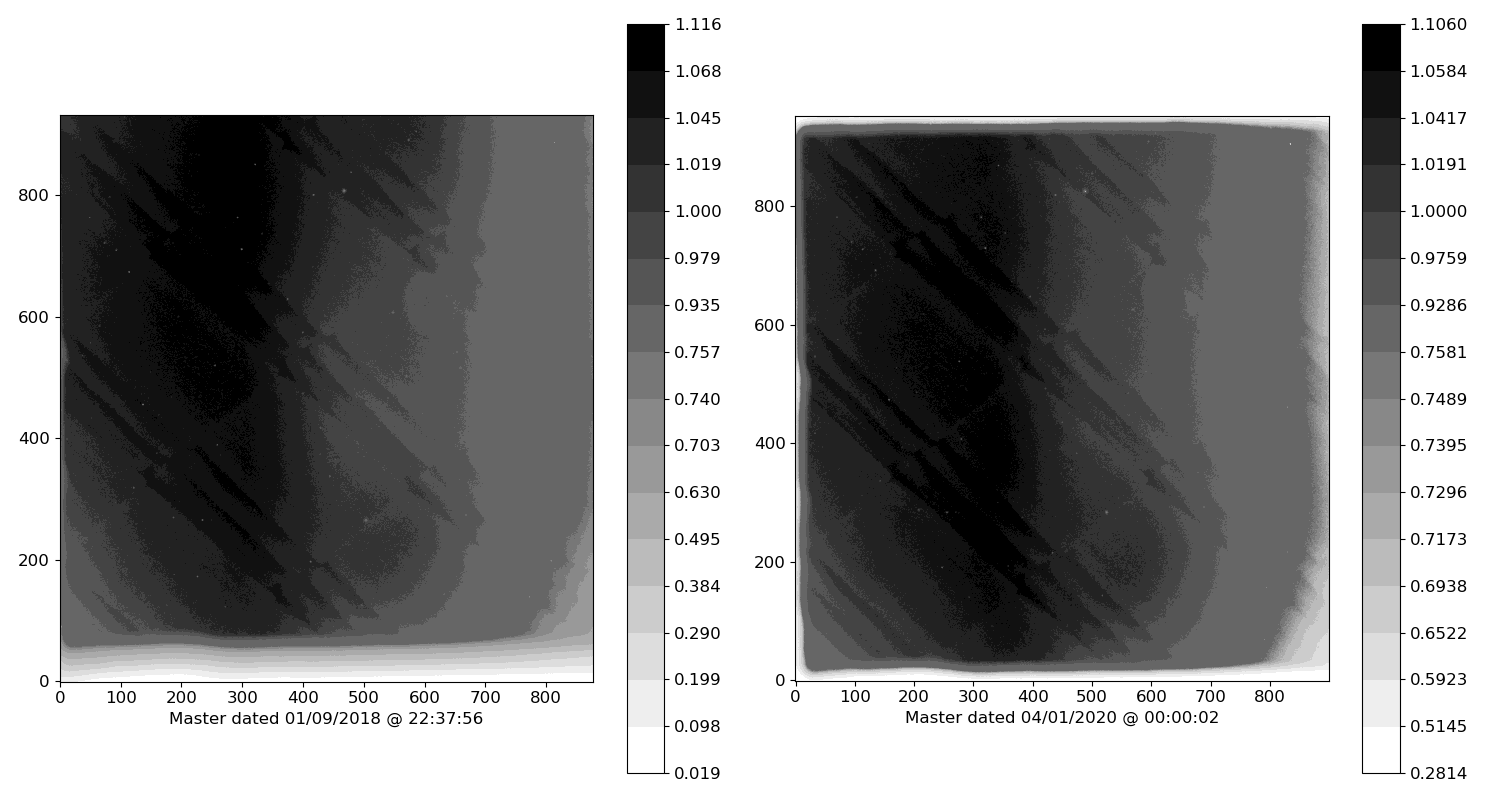
\includegraphics[scale=0.4]{images/complats1820.png}
\end{center}   
\caption{This shows side-by-side the master flat files used to display Fig.
\ref{fig:initgexample} and Fig. \ref{fig:initgexample20}.}
\protect\label{fig:complats1820}
\end{figure}

It might be supposed that this is a problem of the particular pixels concerned.
but if reference is made back to Fig. \ref{fig:showusedccd} earlier it can be
seen that the later observations are taken from a wider area of the CCD than the
earlier ones. For convenience, in Fig. \ref{fig:gfiltareas1820} is shown the
section from Fig. \ref{fig:showusedccd} relating to the \texttt{g} filter and
showing the regions of the CCD used. It can be seen that the area used for the
later observations is larger, especially where the shading is observed at the
bottom of the images. The conclusion reached, and other filters show a
similar story, is that this is more likely to be an issue of the
construction of the telescope, such as vignetting and the like, than problems
with the CCD as the images are set out as projected onto the CCD in these diagrams (there is no rotation of any
image which can be deduced by inspection of sets of observations such as in
Fig. \ref{fig:initgexample} which appear broadly the same). Division by the low
values in these areas will significantly reduce the contrast in the processed
images.

\begin{figure}[!htbp]
\begin{center}
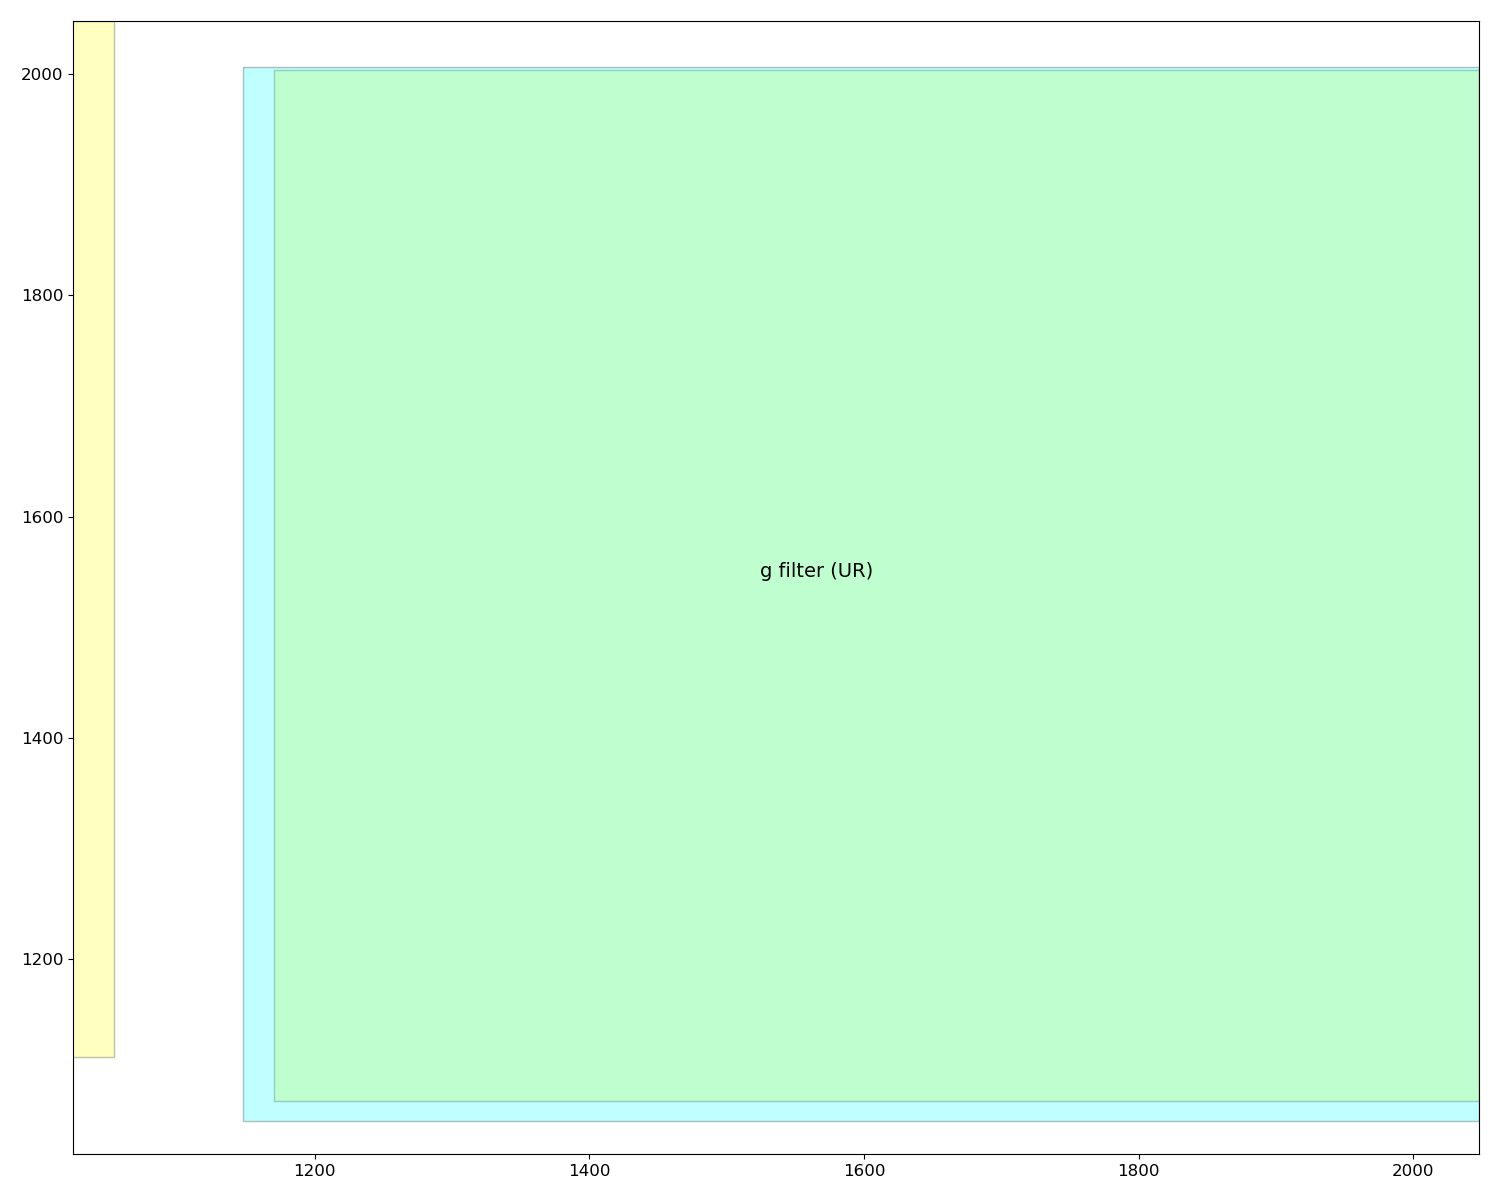
\includegraphics[scale=0.2]{images/gfiltareas1820.png}
\end{center}   
\caption{This is a portion of Fig. \ref{fig:showusedccd} indicating the areas
of the CCD used for the \texttt{g} filter in 2018 and 2020. The cyan region
shows the area used in 2020 and the yellow the area used in 2018. The common
area appears as green. It can be seen that the larger area is that used in 2020
which suggests tat the lower signal seen at the bottom of the image in 2018}
\protect\label{fig:gfiltareas1820}
\end{figure}

As described in \citet{molinari14}, the visible light into the ROSS2 camera is
divided by one dichroic filter into the \texttt{g} and \texttt{r} part and
the \texttt{i} and \texttt{z} parts. Each of those are divided by a further
dichroic filter into the \texttt{g} and \texttt{r} and the \texttt{i} and
\texttt{z} components respectively. Possibly this could be associated with
vignetting or similar brought about by mounting of the dichroic filters. It is
to be noticed that in Fig. \ref{fig:mastfeg0120}, following minor reconfiguration,
this is reduced somewhat.

The master flat files are very similar in content until the reconfiguration in
March 2019. In Fig. \ref{fig:mastmean} is illustrated the mean and standard
deviation of the pixel values in the master flat files over the period of
observation of the {\rdwarf} objects.

\begin{figure}[!htbp]
\begin{center}
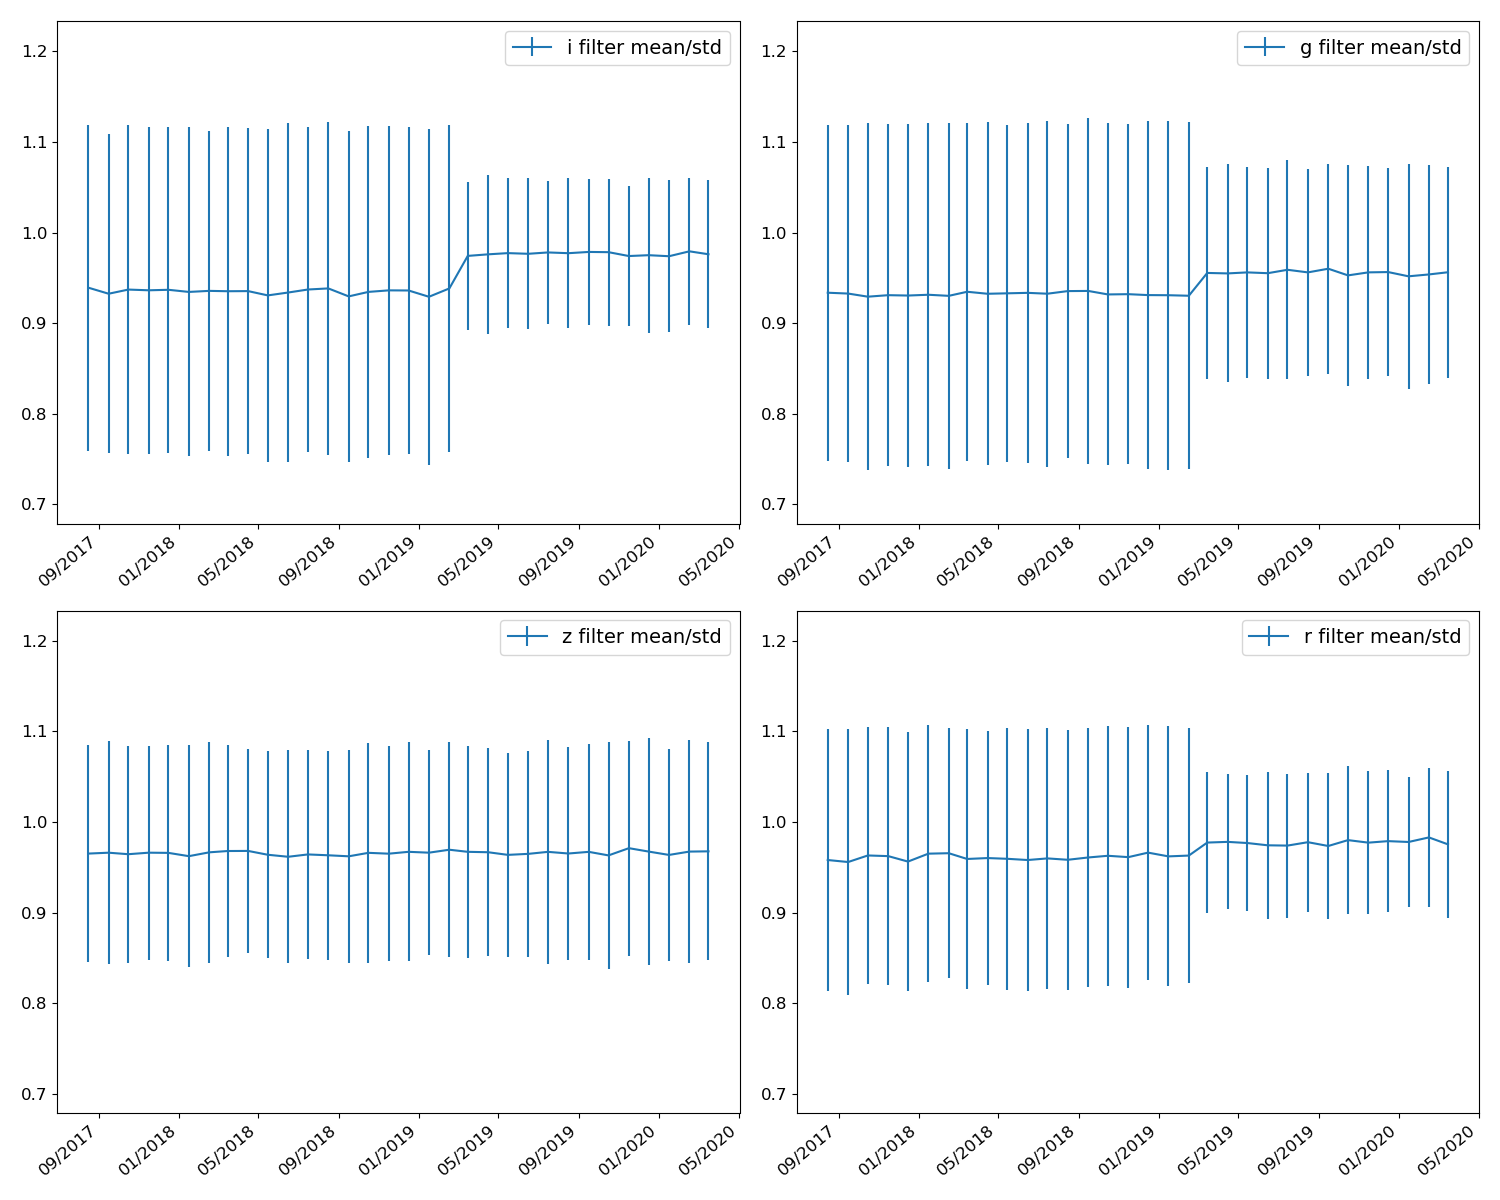
\includegraphics[scale=0.4]{images/mastmean.png}
\end{center}   
\caption{This illustrates the mean and the standard deviation of the values in
the master flat files from July 2017, when {\rdwarf} targets were first
observed, until March 2020. Note the step in March 2019, following
reconfiguration of the telescope.}
\protect\label{fig:mastmean}
\end{figure}

The reconfiguration of the telescope in March 2019 clearly improved the
performance at the edges of the images. It would appear that it would be
desirable to trim the edges of the images, or at the very least give reduced
weighting to photometry taken from these edges.

\subsubsection{Construction of master flat files}
\protect\label{section:constructmff}

Examination of the IDL code used to construct the master flat files revealed
that the master flat files were constructed using the daily flat files for the
relevant month, selected according to the criteria.

\begin{enumerate}
  \item The mean values of the pixel counts falls within the range 5,000 and
  50,000.
  \item The skewness of the distribution of the pixel counts is negative.
  \item The kurtosis of the distribution of the pixel counts is less than 7.
\end{enumerate}

All of these criteria are applied; a daily flat file is not selected if it does
not meet all these criteria. The justification for using the skewness and
kurtosis in this way is not clear.

Regrettably the calculation of the mean, skewness and kurtosis is not correct,
due to a programming error. Further, the history of the master flat file shows
all daily flat files considered for inclusion, not the ones actually selected.
\footnote{It did not seem a productive use of time to reproduce the programming error
and work out the ``correct'' set of daily flat files which went to make up the
master flat files.}

Finally the pixel values are combined by taking the median value and then
normalised. This would appear to be a mistake as the daily flat files are
typically in groups of three as the light fades and thus only values from the
set of ``middle'' flat files would be selected.

The files are normalised to the median value not the mean, as may be apparent
from Fig. \ref{fig:mastmean}, which shows the mean values.

\subsubsection{Daily flat files}
\protect\label{section:dailyflats}

In order to rework the master flat files, a study of the linearity of the daily
flat tiles was undertaken, together with an assessment of the points at which
daily flat files should not be considered towards making a master flat file.

\subsubsubsection{Study of linearity}
\protect\label{section:linearity}
It seemed useful to examine the linearity of the daily flat files by plotting
the standard deviations of of the values for all the pixels in each image against the means.
This is shown in Fig. \ref{fig:dailyflatall}. It would be  expected that this
would be linear with the standard deviations increasing with the mean pixel
values. It is clear from this that there is good linearity up to close to
saturation (at 65,536 counts) but it tails off approaching this. The limits of
5,000 and 50,000 for the mean values in selection of the files for the master
flat files would appear to be  reasonable. However this merits further
investigation, as shown in Section  \ref{section:lincutoff}.

Of concern is that there appear to be two distinct lines in the results three of
the filters. However further investigation showed that this was before and after
the reconfiguration of the telescope in March 2019. Accordingly this was
repeated restricting pixels to those in the common area before and after the
reconfiguration (this appears in green in Fig. \ref{fig:showusedccd}) and correctly
aligning the pixels in the result, with the result as shown in Fig. \ref{fig:dailyflatscomm}.

\begin{figure}[!htbp]
\begin{center}
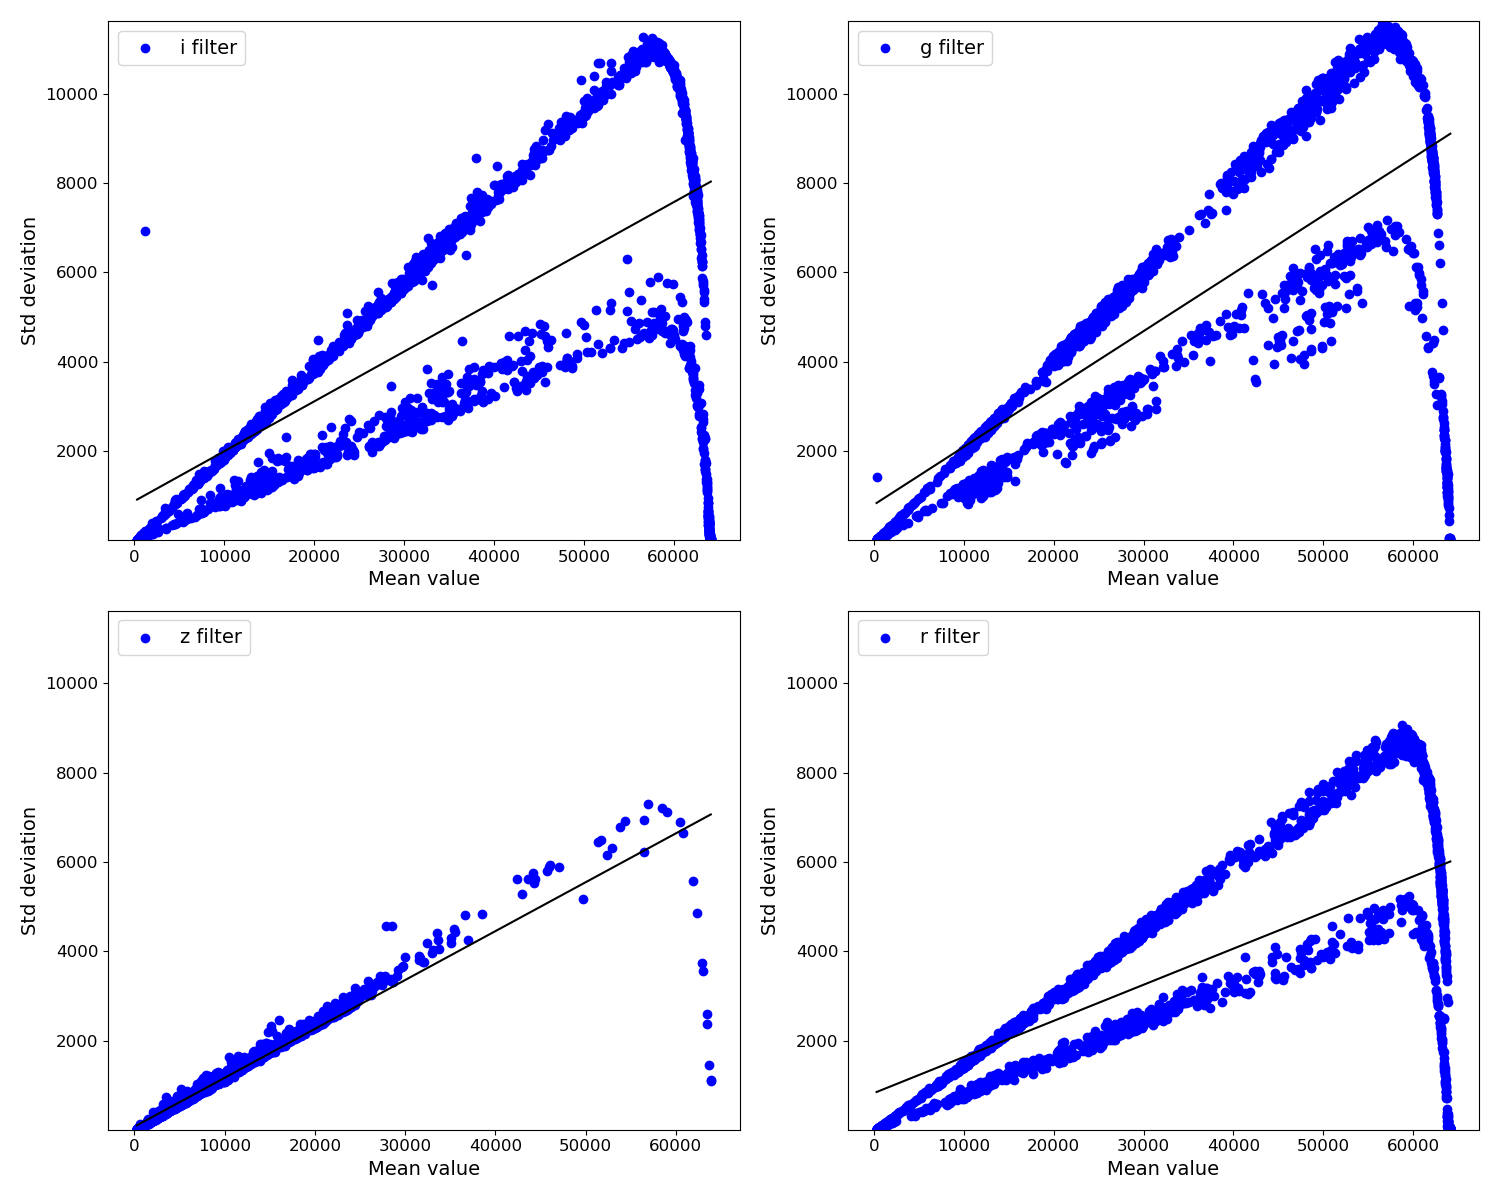
\includegraphics[scale=0.4]{images/dailyflatall.png}
\end{center}   
\caption{This shows the mean plotted against the standard deviations in all
the daily flat files for each of the 4 visible light filters, all to the same
scale. The black line in each case shows the least-squares fit.}
\protect\label{fig:dailyflatall}
\end{figure}

\begin{figure}[!htbp]
\begin{center}
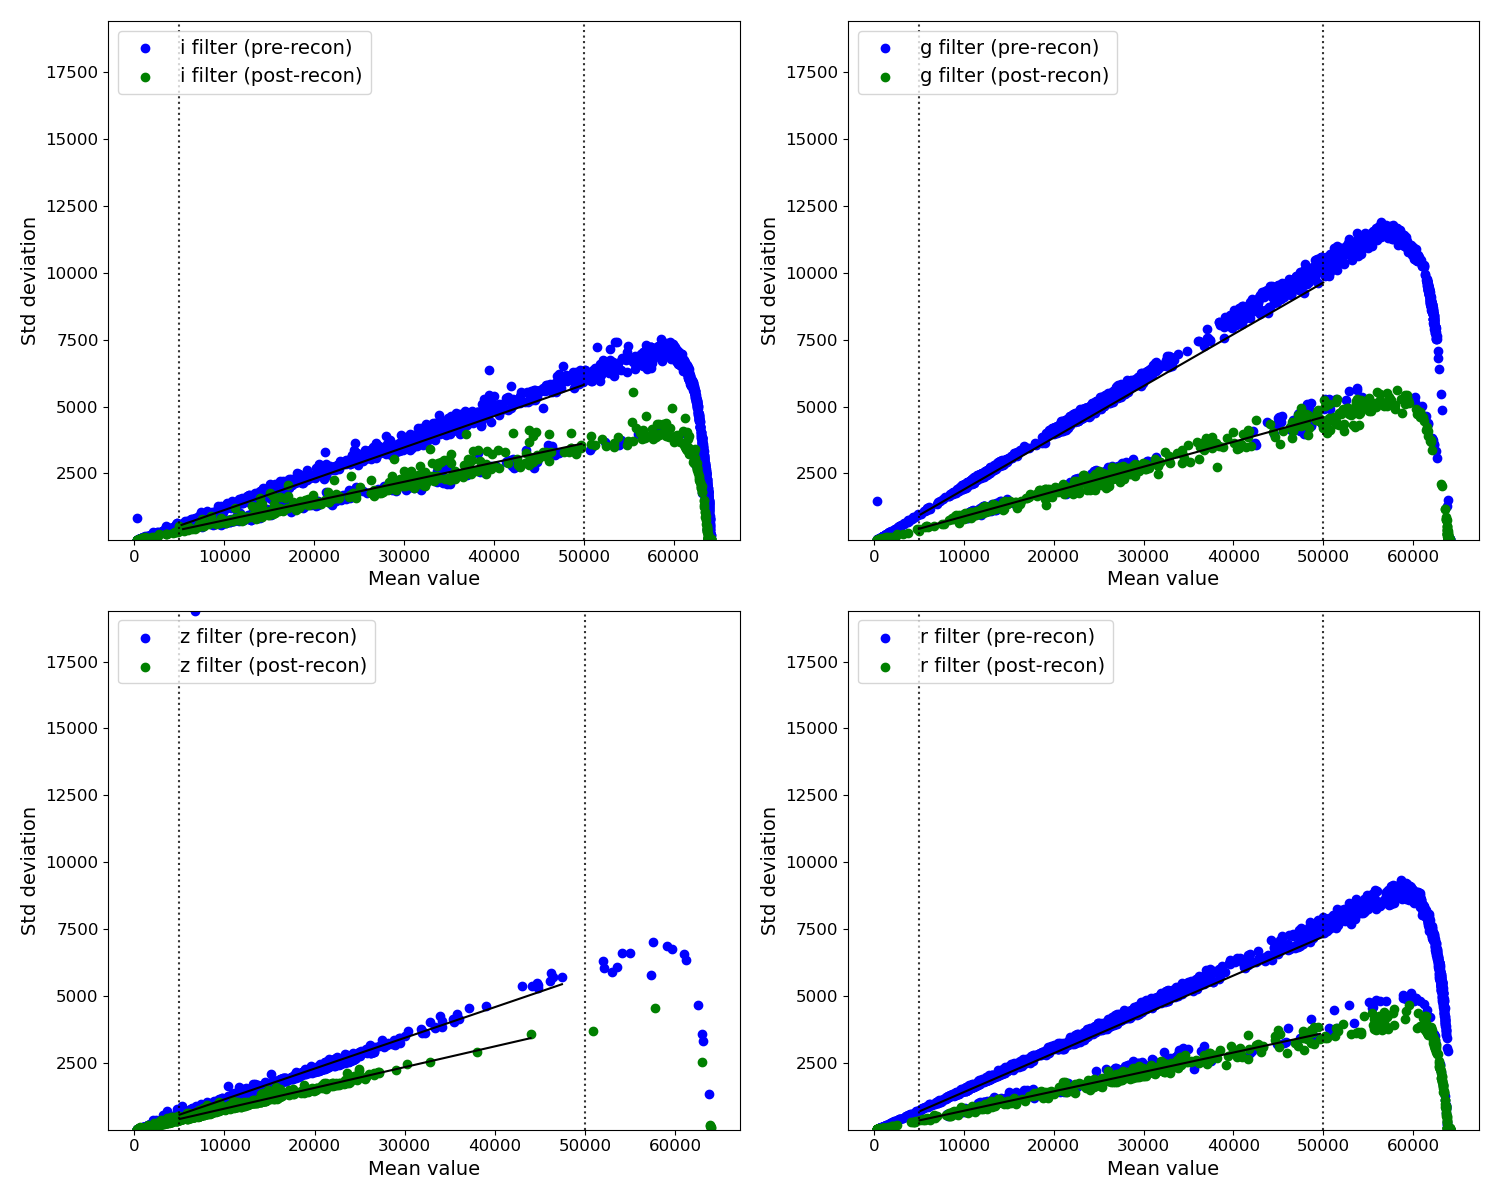
\includegraphics[scale=0.4]{images/dailyflatcomm.png}
\end{center}   
\caption{This figure is equivalent to Fig. \ref{fig:dailyflatall}, but
restricting the pixels to the area of the CCD common to all frames for each
filter and aligning to the same pixels. Points in blue relate to frames taken
prior to March 2019, when the configuration was altered, and those in green
relate to to frames after March 2019. The dotted vertical lines are where the
limits of mean values are taken (at 5,000 to 50,000 counts) in the master flat
files. A least-squares fit was undertaken for frames with mean value within the
limits and this is plotted for each set.}
\protect\label{fig:dailyflatscomm}
\end{figure}

It will be seen from Fig. \ref{fig:mastfeg0918} and Fig. \ref{fig:mastfeg0120}
that the edges tail off, possibly due to vignetting or due to the mounting, do
the plot in Fig. \ref{fig:dailyflatscomm} was repeated for Fig.
\ref{fig:dailyflatstrim}. It will be seen that the linearity agrees much more
substantially. (If the restriction to the common area is not done, this is not
nearly so effective and little difference is made to the display in Fig.
\ref{fig:dailyflatall}.)

\begin{figure}[!htbp]
\begin{center}
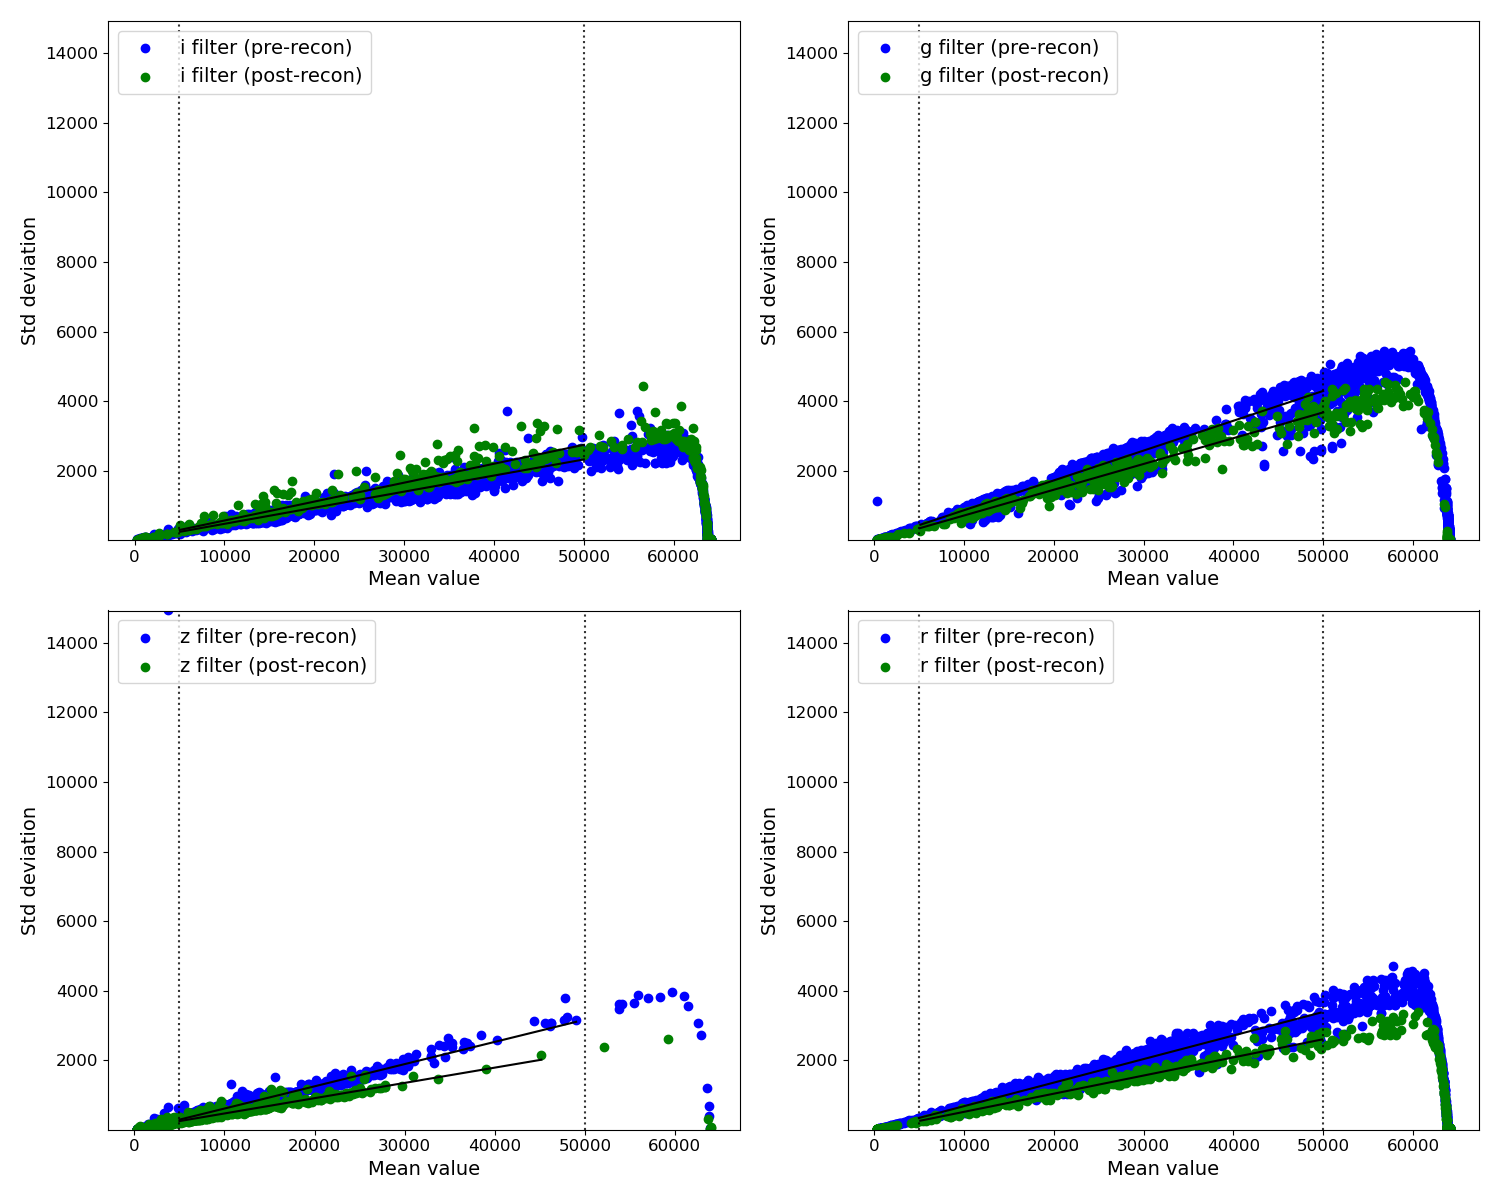
\includegraphics[scale=0.4]{images/dailyflattrim.png}
\end{center}   
\caption{This figure is equivalent to Fig. \ref{fig:dailyflatscomm}, but
additionally 50 pixels are trimmed from each edge of the image.}
\protect\label{fig:dailyflatstrim}
\end{figure}

\subsubsubsection{Linearity cut-offs}
\protect\label{section:lincutoff}

Next examined was the limitation of daily flat files selected for the master
flat to ones with means between 5,000 and 50,000.\footnote{There were other
restrictions, based on the skewness and kurtosis of the distribution, these are
considered further in Section \ref{section:flatselection}.} This was examined by
looking at the correlation coefficients of the fit of the standard deviations to the mean as illustrated in Fig.
\ref{fig:dailyflatscomm} and Fig. \ref{fig:dailyflatstrim}. In Fig.
\ref{fig:lregmaxes} the files are selected with a minimum mean of 10,000 counts
and showing the correlation coefficient of the fig and the standard deviation
with various maximum mean values. In Fig. \ref{fig:lregmins} the daily flat
files are selected with  maximum mean value of 50,000 and various minimum mean
values.

\begin{figure}[!htbp]
\begin{center}
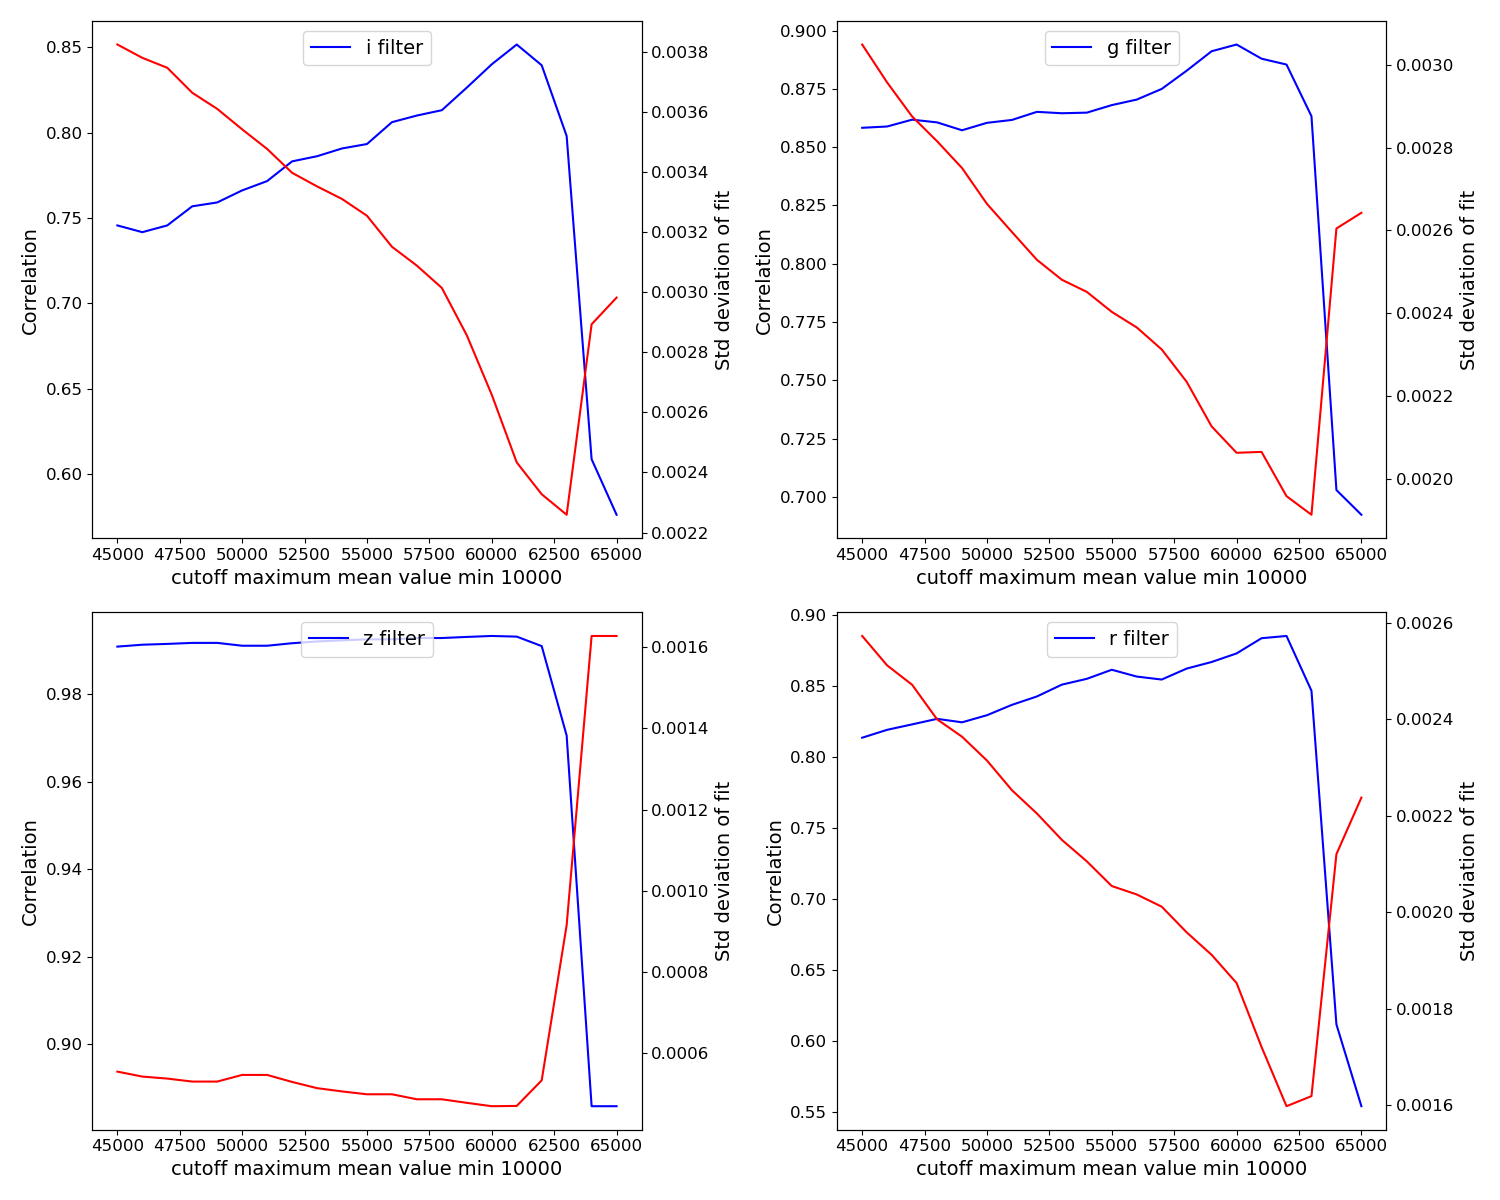
\includegraphics[scale=0.4]{images/lregmaxes.png}
\end{center}   
\caption{This figure was obtained by selecting daily flat files with a minimum
mean value of 10,000 and obtaining the correlation coefficient and standard
deviation of fit with maximum mean value of 45,000 upwards for each filter.}
\protect\label{fig:lregmaxes}
\end{figure}

\begin{figure}[!htbp]
\begin{center}
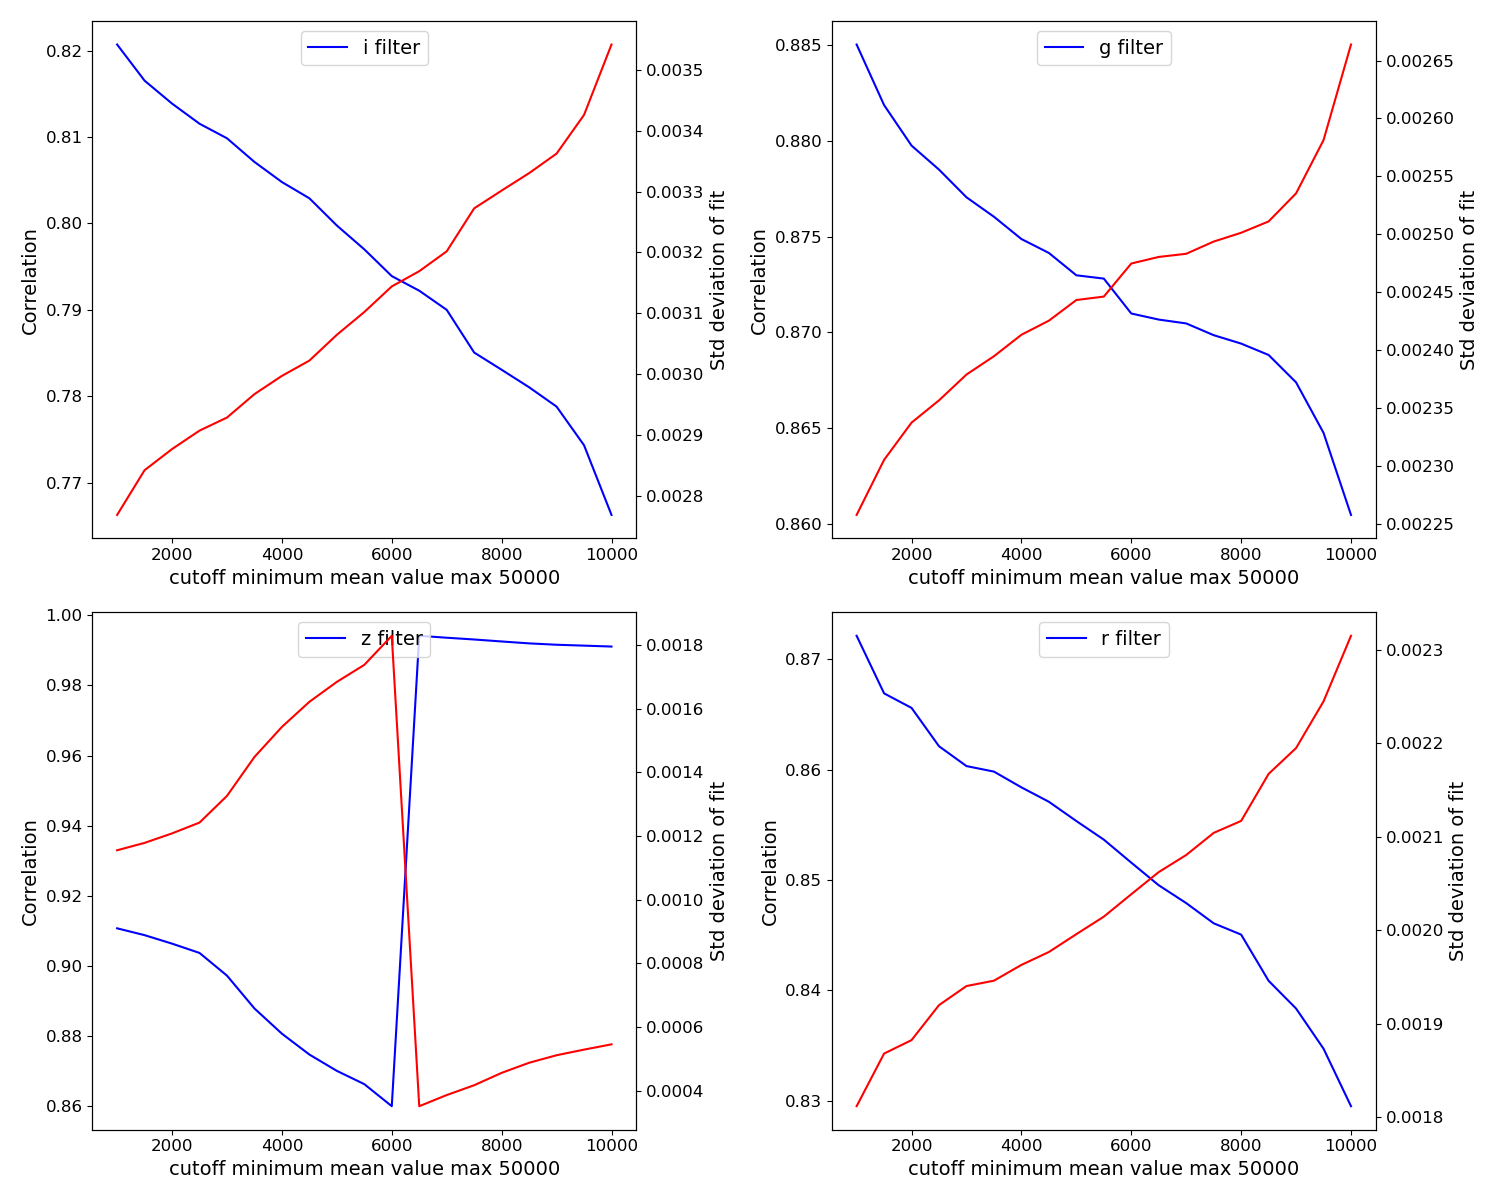
\includegraphics[scale=0.4]{images/lregmins.png}
\end{center}   
\caption{This figure was obtained by selecting daily flat files with a maximum
mean value of 50,000 and obtaining the correlation coefficient and
standard deviation of fit with minimum mean value of 10,000 downwards for each
filter.} \protect\label{fig:lregmins}
\end{figure}

This result might be exactly as expected. As the counts approach the maximum of
65,535, at which the CCD is saturated, the accuracy tails off. At the lower end
of the scale, the signal to noise becomes unacceptably high. It would appear
from these results that a minimum mean of 6,000 would be more appropriate whilst
the maximum mean could safely be raised to 61,000.\footnote{Note that this is
the maximum \underline{mean}, not the maximum \underline{value}, individual
pixels may have a higher value, but frames including the maximum of 65,535 counts should be avoided as
they are likely to be saturated.} Raising the lower level of the mean in this
way would lose the following percentages of daily flat files. It was found that
raising the lower limit of means lost less than 0.5\% of the files, but this was
more than made up for by the increased number of files made eligible for
selection by raising the upper limit to 61,000. This is illustrated in Table
\ref{table:selectedflats}.

The files lost are not seen as particularly significant especially as the files
involved are those with the lowest counts, for which the signal to noise, after
subtraction of the bias files, is inevitably worst. The reverse is true for the
files gained by raising the upper limit.

\subsubsubsection{Selection of daily flat files}
\protect\label{section:flatselection}

With the guidelines taken from the analysis of linearity, it was deemed
appropriate to study the selection of flat files to make up the master flat
files. As stated above in Section \ref{section:constructmff}, this was on the
basis of the means falling within a range of 5,000 to 50,000, together with
further constraints that the skewness of the distribution of pixel values being
negative and the kurtosis being below 7.

In Fig. \ref{fig:flatdispall} are shown the distributions of the means, standard
deviations, skewness and kurtosis for all the daily flat files. If this is
constrained to consider only files with pixel means between 6,000 and 61,000 the
distributions become simpler as shown in Fig. \ref{fig:flatdisplims} and if
files with a standard distribution over 10,000 (representing nearly 20\% of the
maximum pixel value) are omitted, the distributions become as shown in Fig.
\ref{fig:flatdisplimssd10000}.

With reasonable limitations on the flat files, limiting the maximum standard
deviations to 10,000 (it will be clear from \ref{fig:flatdispall} that the
majority are much less than this), that files with positive skewness are reduced
to zero and those with kurtosis over 7 are negligible (under 0.01\%).

It therefore considered that selection based on skewness or kurtosis adds little
benefit\footnote{Even if they were correctly calculated.} and hence for
construction of alternative master flat files, these were omitted.

\begin{figure}[!htbp]
\begin{center}
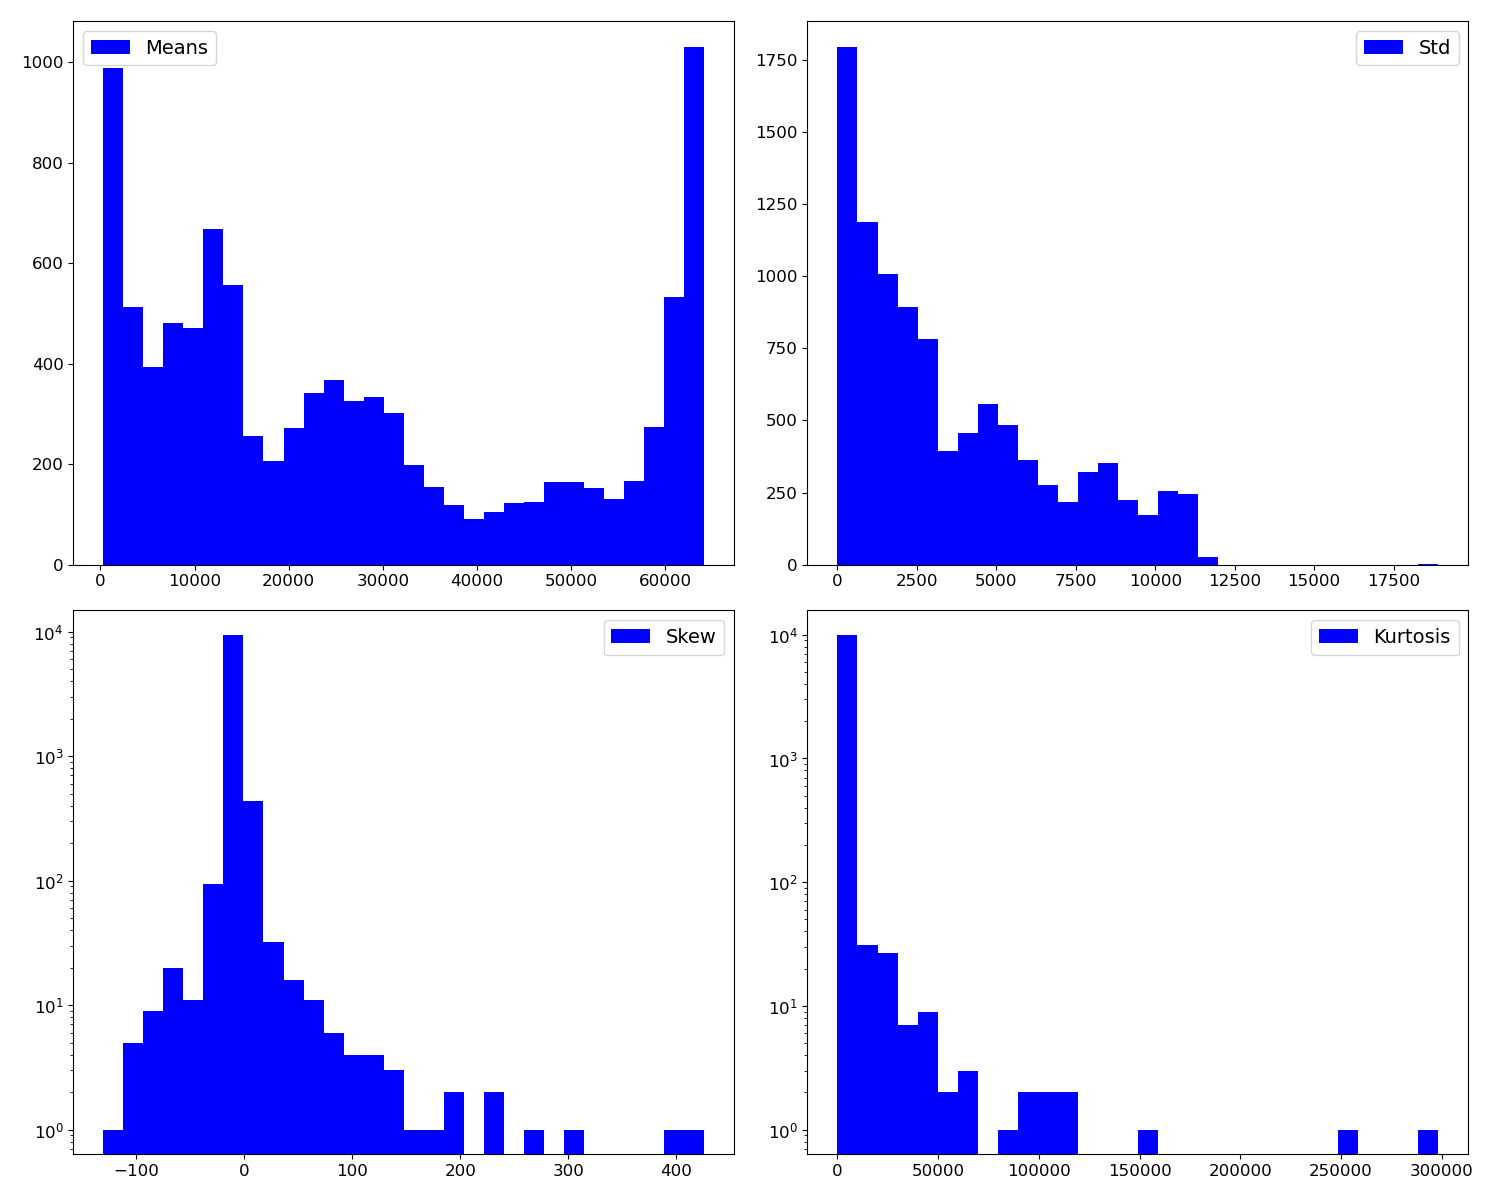
\includegraphics[scale=0.4]{images/flatdispall.png}
\end{center}   
\caption{This figure shows the distribution of means, standard deviations,
skewness and kurtosis of the pixel values of the daily flat files for the
visible light filters. The skewness and kurtosis histogram are displayed on a
logarithmic scale.} \protect\label{fig:flatdispall}
\end{figure}

\begin{figure}[!htbp]
\begin{center}
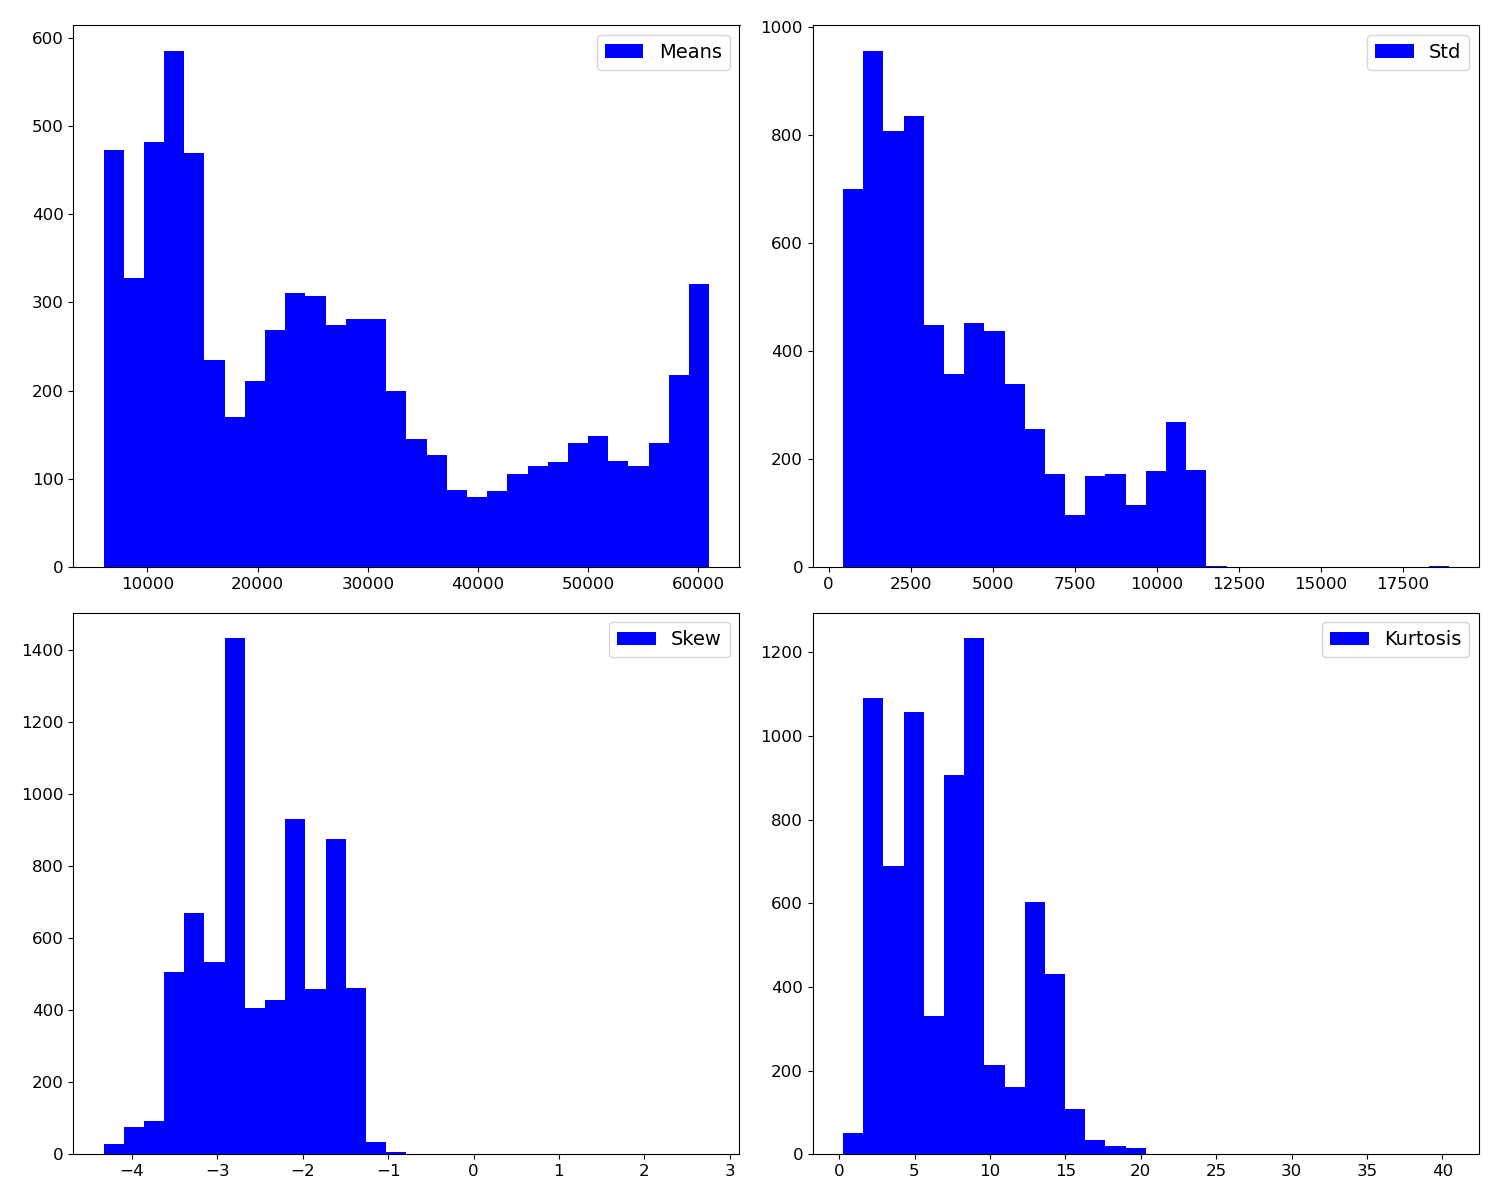
\includegraphics[scale=0.4]{images/flatdisplims.png}
\end{center}   
\caption{This figure is the same data as for Fig. \ref{fig:flatdispall} except
flat files with mean pixel values lower than 6,000 or over 61,000 are
omitted.The skewness and kurtosis are not shown on a logarithmic scale.}
\protect\label{fig:flatdisplims}
\end{figure}

\begin{figure}[!htbp]
\begin{center}
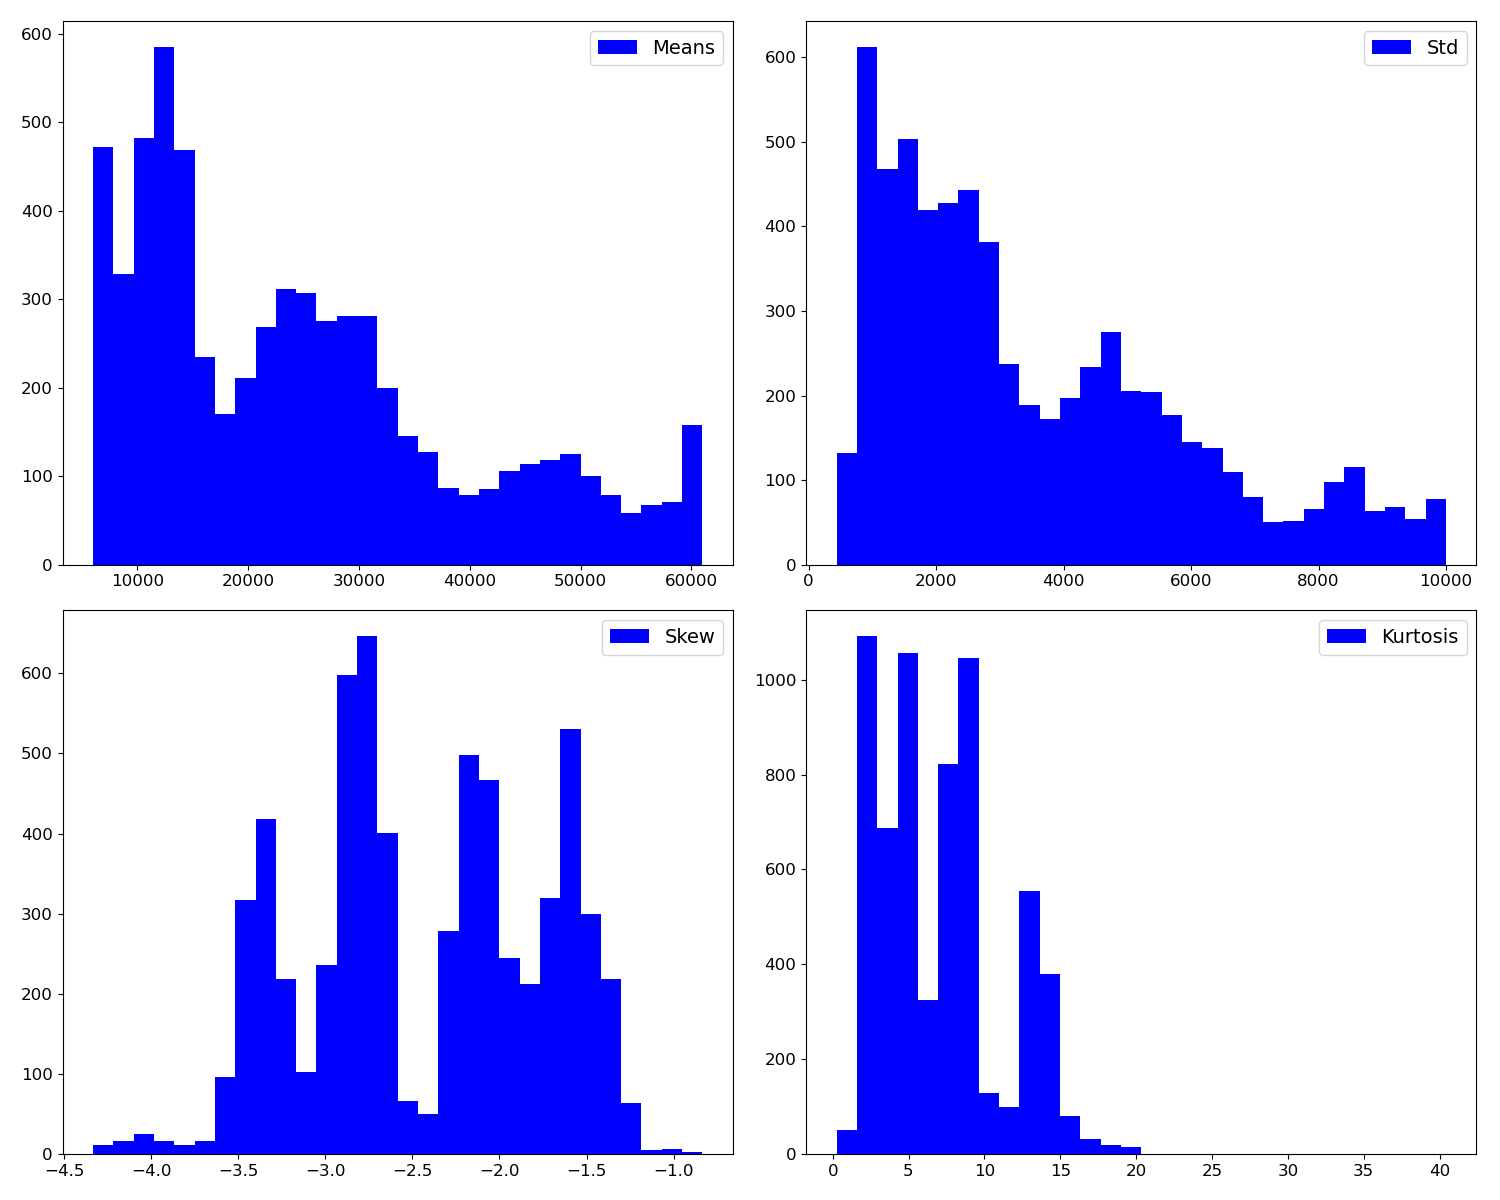
\includegraphics[scale=0.4]{images/flatdisplimssd10000.png}
\end{center}   
\caption{This figure is the same data as for Fig. \ref{fig:flatdisplims} except
additionally flat files with standard deviations over 10,000 are omitted.
The skewness and kurtosis are not shown on a logarithmic scale as they are
distributed more evenly.} \protect\label{fig:flatdisplimssd10000}
\end{figure}
\clearpage

\subsubsection{Creation of alternative master flat files}
\protect\label{seciion:altmasters}

Having determined appropriate alternative criteria, it was appropriate to
consider the construction of alternative master flat files.

The existing master flat files are composed of daily flat files taken from the
preceding month and might consist of files taken 30 days from the relevant
observation date. As with the alternative master bias files as described in
Section \ref{section:dailybiasfiles}, a rolling ``window'' of daily flat files
is used to construct a master flat file tailored to the observation date. 

The existing master flat files were composed by taking the median value for each
pixel from the selected daily flat files and then normalising. As the daily flat
files are taken in groups of three as the light fades but taking the median will
ignore all but the middle set in each case. The benefit of having flat fields
with brighter frames will be lost as well as the darkest flat field frames
(although care must be taken, the signal to noise is lowest on these).

The approach selected was to normalise first and, as the results are ratios
close to 1, combine with a geometric mean.

Unfortunately, this at first presented a problem as the pixels, after
subtraction of the bias files, become zero or negative in some cases, mostly
associated with the lower illumination files, as has also been noted in the
observation files. It is, of course, not possible to calculate a geometric mean
of a sample containing negative or zero values.

However this was first undertaken using the selection criteria used in the
creation of the master flat files, using frames with a mean pixel count between
5,000 and 50,000\footnote{As discussed in section \ref{section:flatselection}
above, the additional skewness and kurtosis restrictions are ignored here.}.

A number of strategies were tried to eliminate flat field images yielding
negative values after subtraction of the master bias images (or alternative
master bias images). These were:

\begin{itemize}
  \item Revision of the selection criteria for flat files as suggested by the
  work in Section \ref{section:flatselection} to those files with means between 6,000 and 61,000
  pixels (the lower limit here being more important for these purposes).
  However this was not completely effective for flat files for the \texttt{z}
  filter. There remained some flat files in 2018, mainly May that still gave
  negative pixels. If the lower limit of means is set to 7,000 for the
  \texttt{z} filter, then the negative pixels are eliminated for the remaining
  files for that filter. However this loses approximately 50\% of the files.
  \item Trim 50 pixels from each edge of the flat field images, however this
  still leaves some flat files for the \texttt{z} filter yielding negative
  pixels.
  \item Eliminate any file with a minimum pixel value below 200 counts (this
  figure was arrived at by considering the mean pixel value over all daily bias
  files of 300). This would lose just over 1\% of all the daily flat files, but
  those would be the files with the poorest signal to noise ratio. Raising the
  threshold to 300 counts would lose just over 2\% of the files and did not
  appear to be necessary.
  \item Eliminate any file with a maximum pixel value above 65,000 counts where
  saturation is approached and the performance is more erratic. This would lose
  about 0.25\% of all the files except for those corresponding to the \texttt{z}
  filter, where 0.5\% of the files would be lost. In only about 5 cases, though
  the same files excluded by these restriction were not excluded by the
  previous restriction of the minimum values.
  \item Apply Gaussian smoothing to each of the daily flat files before
  subtraction of the bias files.
\end{itemize}

It was concluded that the selection criteria to work with for the daily flat
files, taking all these into account, was to restrict selection to the
following.

\begin{itemize}
  \item Frames having mean pixel values to between 6,000 and 61,000.
  \item Frames having minimum pixel values over 200.
  \item Frames having maximum pixel values below 65,000
  \item Frames with standard deviations on pixel values below 10,000.
  \item No consideration of skewness or kurtosis.
\end{itemize}

\textit{I now realise I can do better, including more low light flat files, if
I apply the bad pixels masks first.}

The proportions of daily flat files thereby selected by filter are set out in
Table \ref{table:selectedflats}.

\begin{table}[!htbp]
\begin{center}
\begin{tabular}{lrrr} \hline
Filter & Original & Mean limits & Selected limits\\\hline
\texttt{g} & 30.825 & 75.372 & 69.577\\
\texttt{i} & 36.298 & 68.813 & 63.602\\
\texttt{r} & 36.854 & 66.365 & 66.345\\
\texttt{z} & 58.379 & 60.772 & 60.310\\
\hline
Overall & 40.589 & 67.830 & 64.958\\

\hline
\end{tabular}
\end{center}
\caption{This shows the percentages of daily flat files eligible for selection
for each filter (first column) using the original criteria (second column),
just changing the range of means (third column) and the criteria finally
selected, limiting flat fields with maximum pixel values less than 65,000,
minimum values greater than 200 and standard deviation less than 10,000.}.
\protect\label{table:selectedflats}
\end{table}
\clearpage

\subsection{Hotspots or defective pixels}
\protect\label{section:hotspots}

A study was undertaken of all the files, flat files, bias files and observation
files to determine whether any pixels in the CCD array could be counted as
``bad'' or unresponsive, had particularly high mean values or large standard
deviation. The literature varies somewhat on how bad pixels are defined or
determined.

Of recent papers, \citet{allers20} define bad pixels as ``dead'' pixels or pixels
with an uncertainty in the flat fields of over 10\%. In \citet{piskunov20} bad
columns in the CCD used are first identified and eliminated and then an
iterative procedure is adopted to effectively assign weights to each pixel. In
\citet{bongiovanni19} a procedure based on constructing two composite flat
fields from low and high counts and regarding as bad the pixels where the ratios
differ by more than 15\%. In \citet{belli18} a bad pixel mask is constructed by
selecting pixels in the flat fields with very low counts and those in the dark
frames with very high counts (but the criteria for ``low'' and ``high'' counts
in those files are not defined). In \citet{briesemeister18} pixels in the
constructed flat fields with values less than 0.5 or greater than 1.5 are
considered to be bad.

A comprehensive study of the quality of pixels is described in the
recently-published \citet{maslennikova20}. Pixels are described as
\textbf{Normal}, \textbf{Cold}. \textbf{Warm}. \textbf{Dead}, \textbf{Hot} and
\textbf{Inverse} according to the responses. The pixels on the ROSS2 telescope
CCD do not fit neatly into these brackets, apart from the \textbf{Normal} ones.

For the purposes of this study, the following definitions are used.

\begin{description}
\item[Normal] pixels are those which are clearly well-behaved with a linear
response within 10\% of saturation.
\item[Bad] pixels are closest to \textbf{Dead} pixels as defined in 
\citet{maslennikova20}. Included are those with consistent high levels of noise,
with the standard deviation on the bias level over 5 times the standard
deviation and those.
\item[Unreliable] pixels are ones which whilst otherwise normal, can randomly
give very high or low readings.
\end{description}

There are very few examples, in the order of 25 pixels spread over the used area
of the array, which qualify as \textbf{bad}, but the pixels which are
\textbf{unreliable} are of the order of about 11,000 over the array, spread over
the 4 areas used.

\subsubsection{Total bad pixel statistics}
\protect\label{section:totalbadpix}

\textit{I'm going to display totals for bad pixels for each filter before and
after reconfiguration in March 2019 and also showing any overlaps.}

\subsection{Results after callbartion revisions}
\protect\label{section:postcalibration}

\textit{I need to write this section to show the improvements made to the
displays in Fig. \ref{fig:initgexample} etc and elimination of negative pixels
via these efforts. The full treatment of bad pixels probably means that I can
include more daily flat files excluded previously due to negative pixels.}

\clearpage
 
% \subsection{Flat files}
% \protect\label{section:flatfiles}
% 
% Two kinds of flat file are provided, a set of daily flat files for each of the
% filters, typically 2 or 3 each day for each of the 4 visible light filters \textbf{g},
% \textbf{i}, \textbf{r} and \textbf{z} and for gains of 1 and 4 and the monthly
% master flat files, consisting of a composite of the daily flat files for the
% month.
% 
% \subsubsection{Daily flat files}
% \protect\label{section:dailyflatfiles}
% 
% The daily flat files, after the end of 2013, which precedes the first of the
% observations, are taken with an exposure time of 1 second. Some have a gain of
% 4.4, in line with the gain applied to some of the other observations, but in
% this report only the flat files with a gain of 1 are considered as all the
% observations of the 3 target stars were taken with a gain of 1.
% The master flat files are only taken from these. Usually (but not always) three
% flat files are taken will decreasing light. In Fig. \ref{fig:giflat} are shown
% typical daily flats for the \texttt{g} and \texttt{i} filters, and in Fig.
% \ref{fig:rzflat} are shown similar ones for the \texttt{r} and \texttt{z}
% filters.
% 
% \begin{figure}[!htbp]
% \begin{center}
% %\includegraphics[scale=.4]{images/giflat.png}
% \end{center}   
% \caption{These are examples of two typical daily flat files for the \texttt{g}
% and \texttt{i} filters.}
% \protect\label{fig:giflat}
% \end{figure}
% 
% \begin{figure}[!htbp]
% \begin{center}
% %\includegraphics[scale=.4]{images/rzflat.png}
% \end{center}   
% \caption{These are examples of two typical daily flat files for the \texttt{r}
% and \texttt{z} filters.}
% \protect\label{fig:rzflat}
% \end{figure}
% Rows and columns of the image containing zero pixels were removed from the
% images before analysis. These values are replaced by \texttt{NaN} in the master
% flat files and correspond to invalid pixels. They cannot be used in computations
% as the pixels in the object are divided by the same pixel corresponding flat
% file which would entail division by zero.
% 
% It was of concern that many of the daily flat files had pixels which were vary
% close to saturation. in some cases they were clearly saturated, but none of the
% master flat files appeared to incorporate the daily flat files with definitely
% saturated pixels. In Table \ref{table:satpix} is shown the proportion of
% nearly saturated pixels in flat files for each filter.
% 
% \begin{table}[!htbp]
% \begin{center}
% \begin{tabular}{lrrr} \hline
% Filter & Flat files & Saturated & Over 50\%\\\hline
% g & 3,679 & 29.49 & 22.34 \\
% i & 3,679 & 32.37 & 27.43 \\
% r & 3,680 & 32.66 & 28.12 \\
% z & 3,680 & 0.92 & 0.60 \\\hline
% Overall & 14,718 & 23.86 & 19.62\\
% \hline
% \end{tabular}
% \end{center}
% \caption{Breakdown of daily flat files by filter up to August 2019 showing
% number, percentage with nearly saturated pixels present and percentage with over
% 50\% saturated pixels (in many cases this was over 90\% and occasionally 100\%).}
% \protect\label{table:satpix}
% \end{table}
% 
% \subsubsection{Linearity of CCDs}
% 
% It might be reasonable to expect that if the CCDs are linear, then the standard
% deviation of the values in the daily flat files would rise in proportion to the
% mean values in the daily flat files. In Fig. \ref{fig:ffcorr} is shown how this
% correlates for the four filters.
% 
% \begin{figure}[!htbp]
% \begin{center}
% %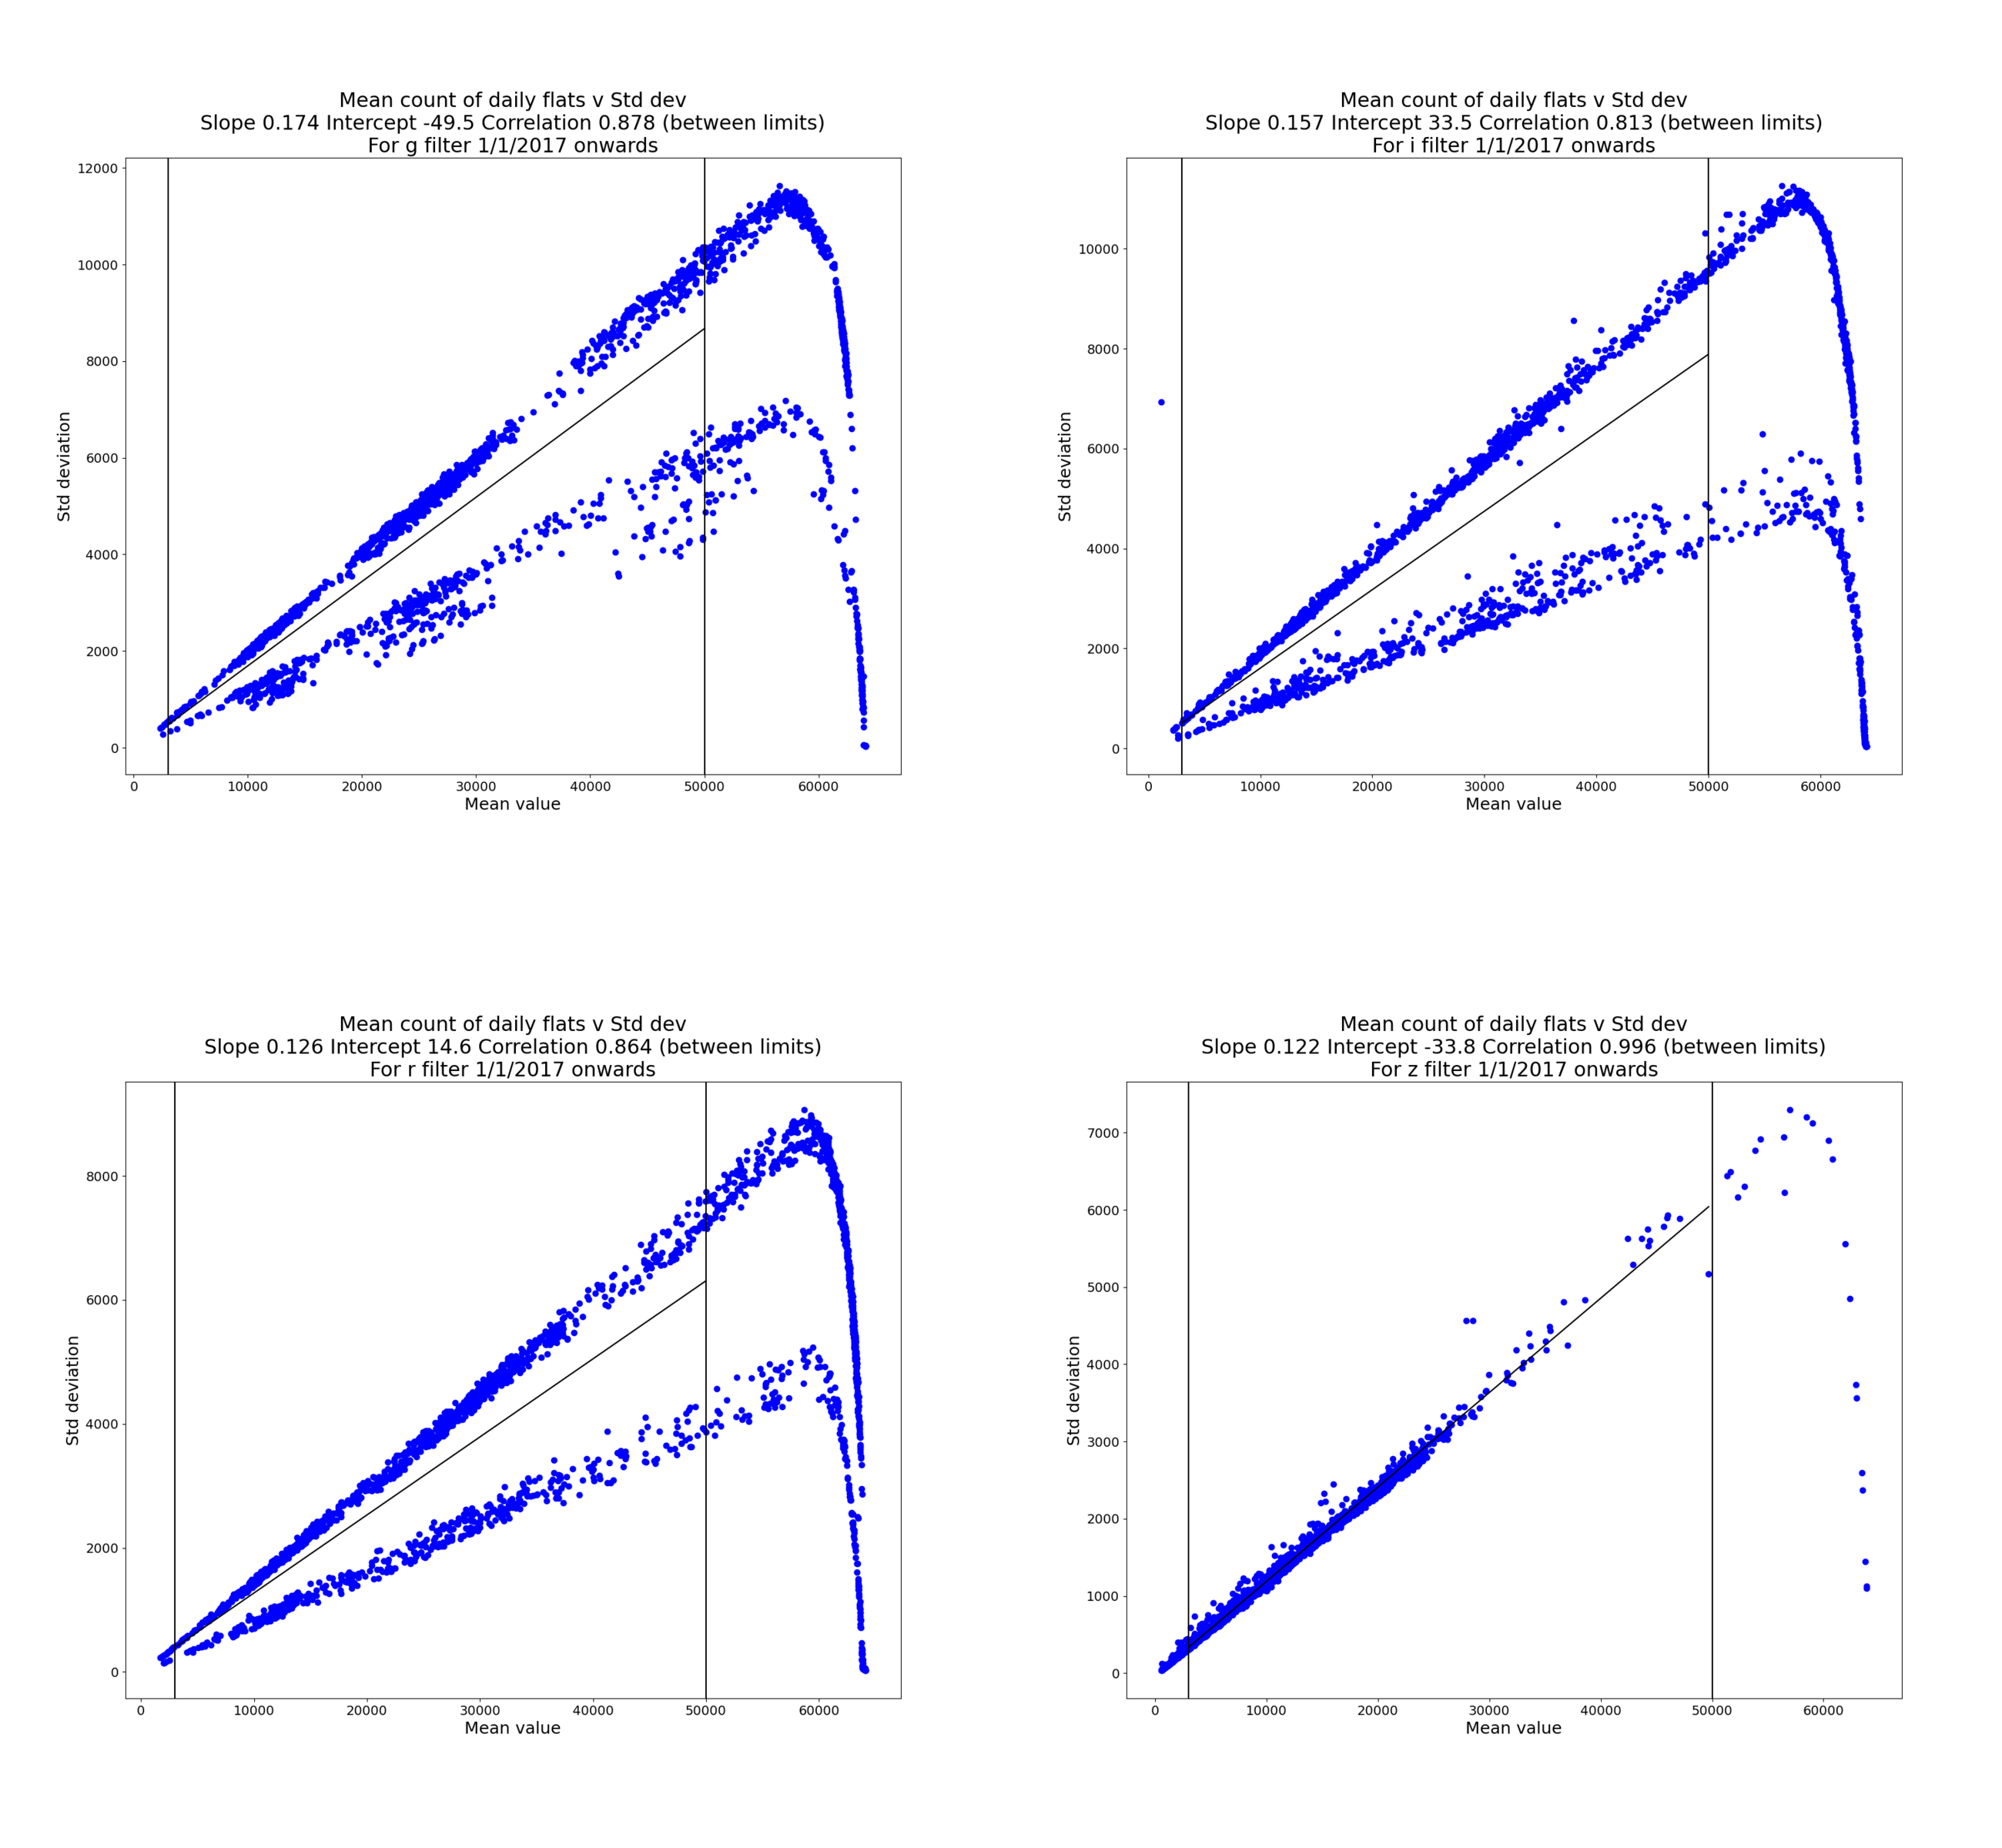
\includegraphics[scale=0.2]{images/corr.png} \\
% \end{center}   
% \caption{This figure shows how the standard deviation of the values in the
% daily flat files corresponds to the four filters. In the top is shown the
% results for the \texttt{g} filter, the bottom left shows the \texttt{r} filter,
% the top right shows the results for the \texttt{i} filter and the bottom right
% shows the results for the \texttt{z} filter. The black line shows the best fit
% slope in each case. The black vertical lines show the upper and lower limits of
% the selection originally used in the master flat files, i.e. mean between 5,000
% and 50,000. Calculation of the best fit slope is restricted to values between
% those limits.}
% \protect\label{fig:ffcorr}
% \end{figure}
% 
% The master flat files are built from flat files with means between 5,000 and
% 50,000, which would appear to be a reasonable choice, the linearity drops off
% dramatically as saturation is reached in all cases.
% %\
% \subsubsection{Master flat files}
% \protect\label{section:masterflatfiles}
% 
% The master flat files consist of median values of the incorporated daily flat
% files, the header indicating which ones are considered.
% 
% Invalid pixel values are represented by \texttt{Nan} and rows and columns
% containing these values are trimmed from the images, both for the flat files
% themselves, and also for the corresponding bias and observations files.
% 
% The program used to create the master flat files selects daily flat files with a
% mean value between 5,000 and 50,000 \textbf{and} with a negative skew and
% kurtosis less than 7. It seemed probable that this latter restriction was a
% mistake and ``\textbf{or}'' was intended
% 
% It would appear to the author that the upper limit is too great and several
% files with saturated pixels are included, using the median pixel value will
% exclude these, but this creates a difficulty in that as 3 daily flat files are
% taken from the sky before observations start, effectively the middle one is
% taken in each case by the median.
% 
% It appeared that each daily flat file should
% be normalised first and the results combined, so a procedure to create
% alternative master flat files was devised. This turned out to be compromised by
% the extreme values in the bias files, which made some of the pixel values
% negative in the daily flat files before normalisation. The issues identified in
% Section \ref{section:hotspots} will have to be properly addressed in order to
% make progress here. The reason that the original master bias files were not
% affected by the negative pixel problem is that they were combined, with much
% higher individual pixel values, before normalisation not afterwards. The negative
% pixel values occur when the lowest light level daily flat file has the bias
% value subtracted before normalisation.
% 
% It was noticed that there was a computational error in the calculation of the
% mean, standard deviation and other parameters in the master flat files and these
% had to be discarded in any event. As the daily flat files change somewhat over
% time reliance on a master flat file possibly
% 30 days removed from the observations to which it relates would seem
% inappropriate and a procedure of ``rolling'' master flat files centred on the
% observation dated was adopted, but this cannot be proceeded until the problem of
% negative pixels in the daily flat files is resolved.

\subsubsection{Accuracy}
\protect\label{section:accuracy}

\textit{This probably wants moving somewhere else to a later section on
modifications to the REM telescope.}

Combination of daily bias values clearly improves the accuracy. The median
pixel value for all of the bias files for all of the filters is approximately
300 with a standard deviation of about 7 for the individual files, 3 for where
all the daily ones for a given day are merged and 1 for the master bias files.

It seemed worth looking at whether any adjustments of the exposure times might
improve the accuracy, as many of the objects which might be used for reference
give an ADU count only just above the sky level. The exposure times currently
are 10 seconds for {\prox} and Ross 154 and 5 seconds for \bstar.

Table \ref{table:pixvals} is set out the maximum value in any of the observation
files for each target and each filter and the percentage of observation files in
which at least one pixel exceeds a give number of ADUs (this does not currently
take account of defective pixels or cosmics, but these would have negligible
effects on the results).

It is clear that some increase in exposure time, possibly up to 5 times or more
in the case of the \texttt{g} filter, would benefit the contrast, except
for the \texttt{i} filter results, which are generally too close to saturation.
The nature of the instrument, however, may not permit any different exposure
times to be made with different filters.

\begin{table}[!htbp]
\begin{center}
\begin{tabular}{|l|r|rrrr|} \hline
Filter & Max value & \% over 30,000 & \% over 40,000 & \% over 50,000 & \% over
60,000 \\\hline
 \multicolumn{6}{|c|}{\textbf{\bstar} exp 5 sec} \\\hline
\texttt{g} & 63,422 & 0.05 & 0.05 & 0.05 & 0.05 \\
\texttt{i} & 63,448 & 78.94 & 61.15 & 45.71 & 0.77 \\
\texttt{r} & 54,806 & 16.68 & 3.73 & 0.97 & 0.00 \\
\texttt{z} & 63,387 & 12.52 & 3.37 & 0.87 & 0.05 \\
\hline
\multicolumn{6}{|c|}{\textbf{\prox} exp 10 sec} \\\hline
\texttt{g} & 63,466 & 0.38 & 0.30 & 0.25 & 0.18 \\
\texttt{i} & 63,457 & 74.15 & 52.88 & 36.84 & 4.03 \\
\texttt{r} & 63,425 & 0.60 & 0.10 & 0.09 & 0.08 \\
\texttt{z} & 63,456 & 25.38 & 11.64 & 5.47 & 0.16 \\
\hline
\multicolumn{6}{|c|}{\textbf{Ross 154} exp 10 sec} \\\hline
\texttt{g} & 63,453 & 0.41 & 0.35 & 0.28 & 0.22 \\
\texttt{i} & 63,452 & 76.71 & 57.35 & 39.25 & 2.16 \\
\texttt{r} & 63,268 & 7.99 & 2.38 & 0.93 & 0.11 \\
\texttt{z} & 63,447 & 8.33 & 2.14 & 0.45 & 0.04 \\
\hline
\hline
\end{tabular}
\end{center}
\caption{This figures shows the maximum ADU values of any pixel in any of the
observation files for each of the 3 {\rdwarf} targets for each filter. The
following columns show the percentage of pixels in each case which are above
30,000, 40,000, 50,000 and 60,000.}.
\protect\label{table:pixvals}
\end{table}
\clearpage

% \subsection{Analysis of images}
% \protect\label{section:analimages}
% 
% \textbf{Please note that since I realised that the master flat files are not
% normalised as Luciano told me I'll have to redo all this. The results within
% each month are consistent but not with other months. Also with the flat files
% properly normalised some of the images will have greater contrast.}
% 
% \subsubsection{Intensity comparison}
% \protect\label{section:intcomp}
% 
% As a first attempt to study the data, the ADU count was taken, specifically the
% net after applying the flat and bias files of the target in all the images in which it was available.
% The target was found in all of the images, apart from in a few of the
% \textbf{g}, \textbf{i} and \textbf{r} visible light filters,
%, as shown in Table
%\ref{table:occtb} below.

%Plotting light curves of the intensities obtained in this way yields Fig.
% \ref{fig:allall}.
%Binning the intensities together into a single day gave
%Fig. \ref{fig:allbin}, the error bars indicate the spread over a single day.

%I plotted
%periodograms, as shown in Fig. \ref{fig:pgrams}. Despite the crudeness of the
%data, it is noticeable that there are peaks close to the rotation periods of
% the order of 150 days referred to in \citet{suarezmascareno15} and \citet{toledopadron18}.

% \begin{figure}[!htbp]
% \begin{center}
% 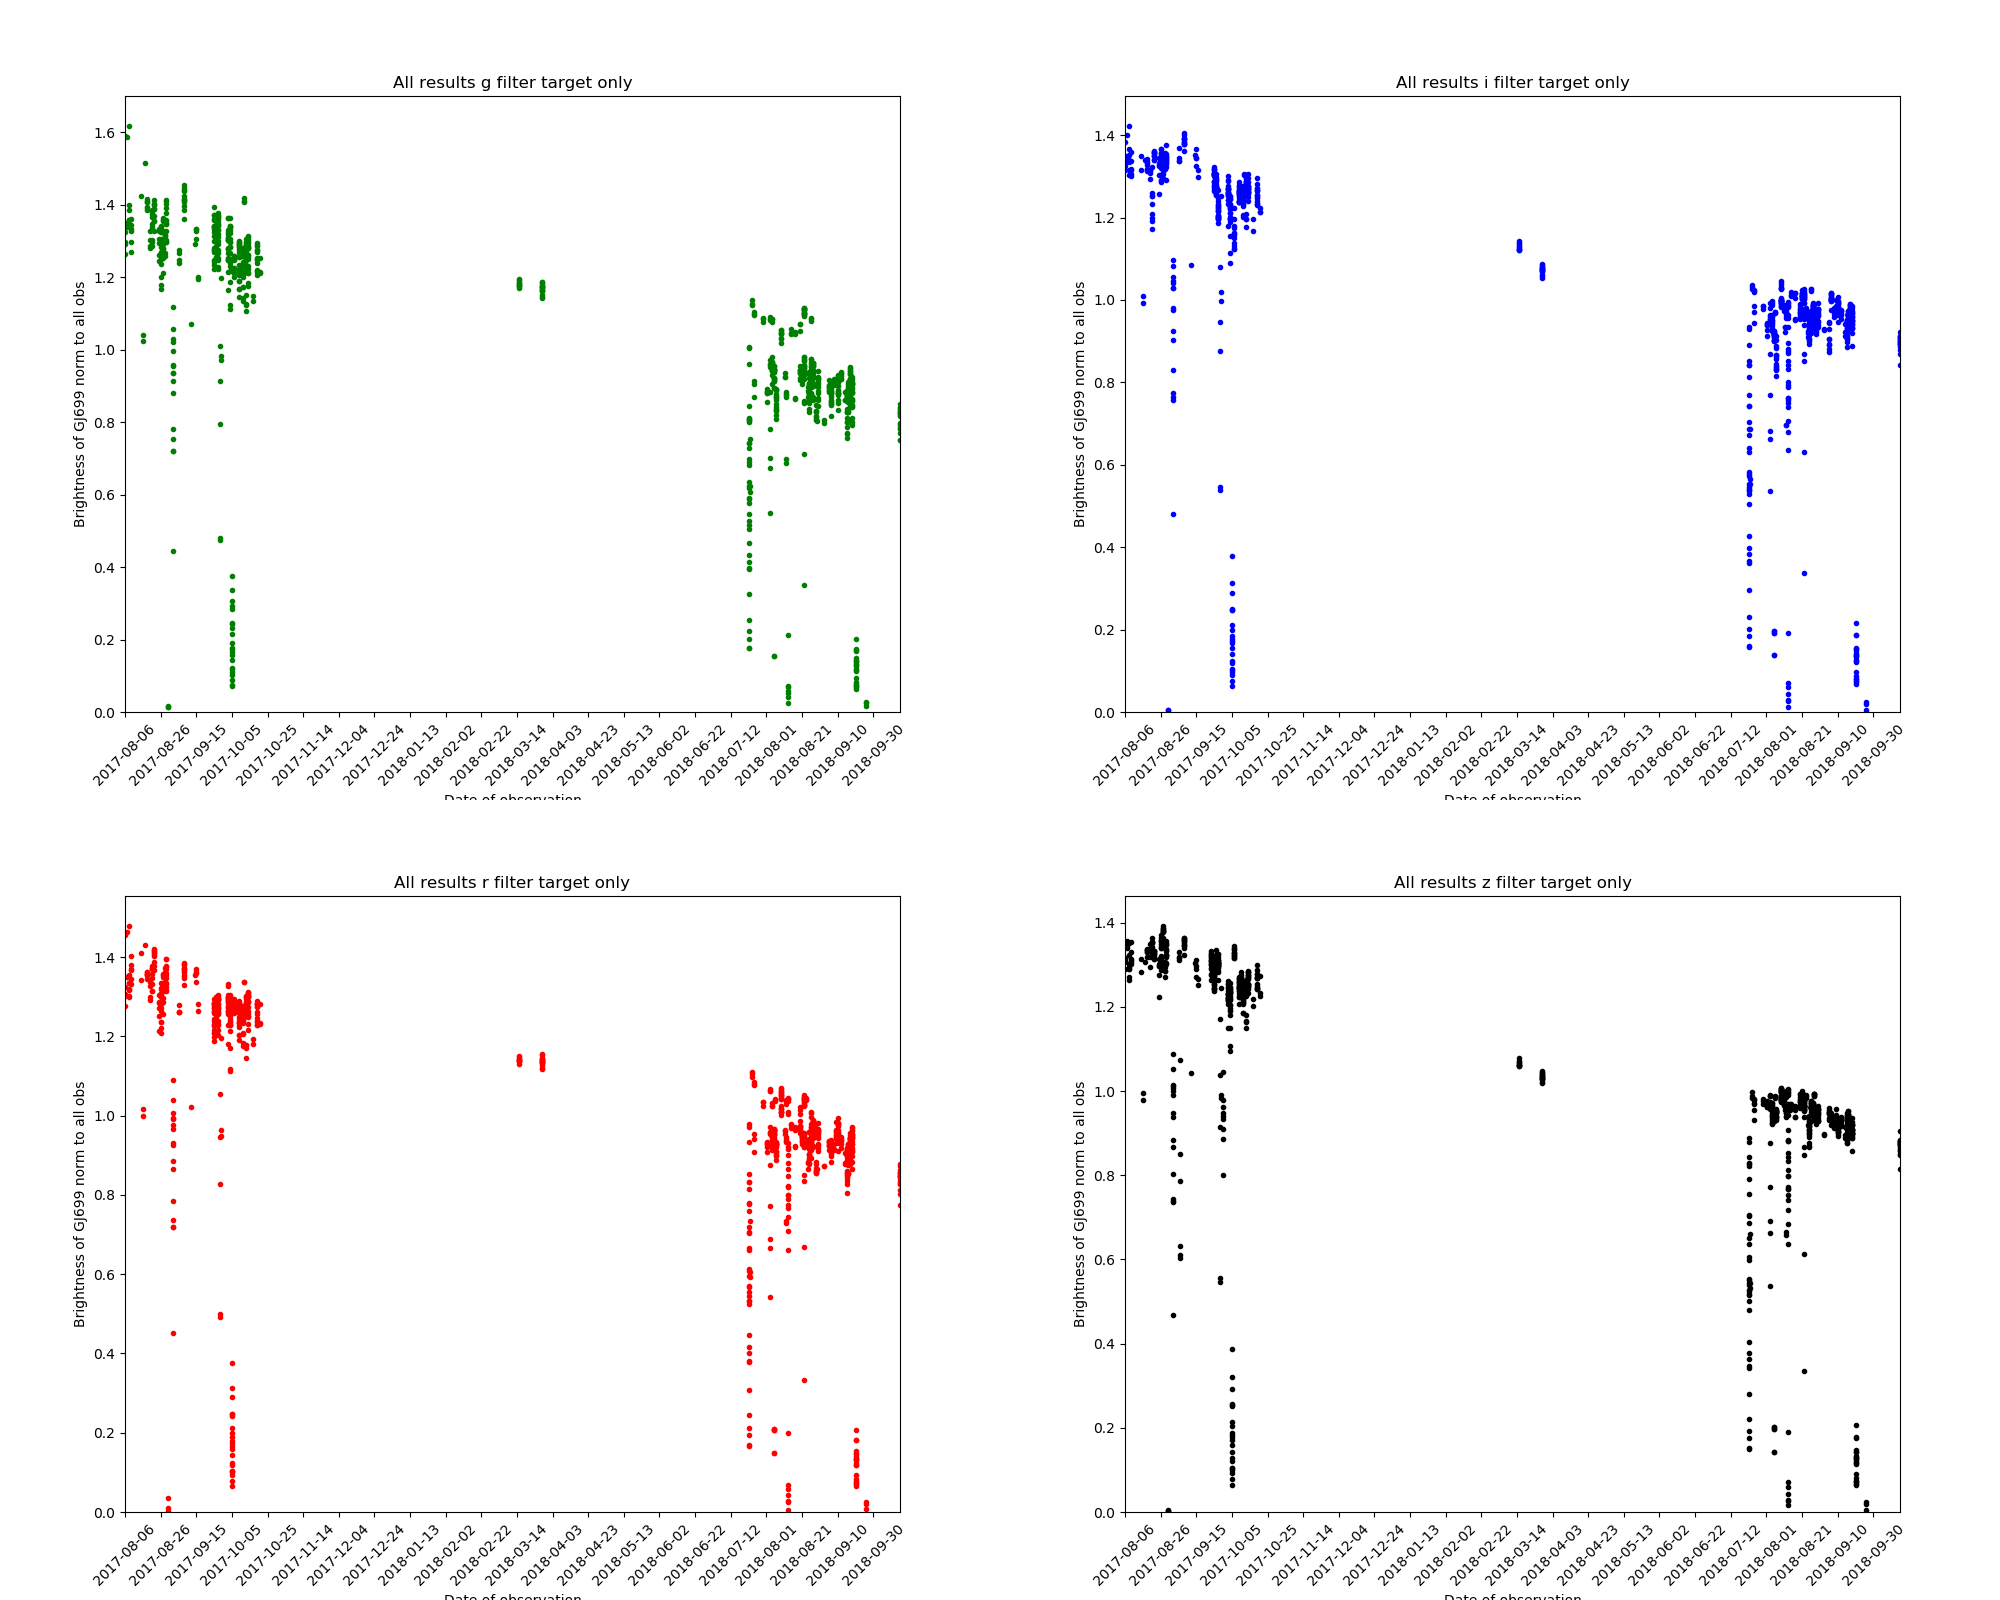
\includegraphics[scale=0.25]{images/allall.png} \\
% \end{center}   
% \caption{This shows the flux for the target, \bstar, for each of the four visible light filters. This takes the total
%   ADU count only}
%   \protect\label{fig:allall}
% \end{figure}
% 
% \begin{figure}[!htbp]
% \begin{center}
% 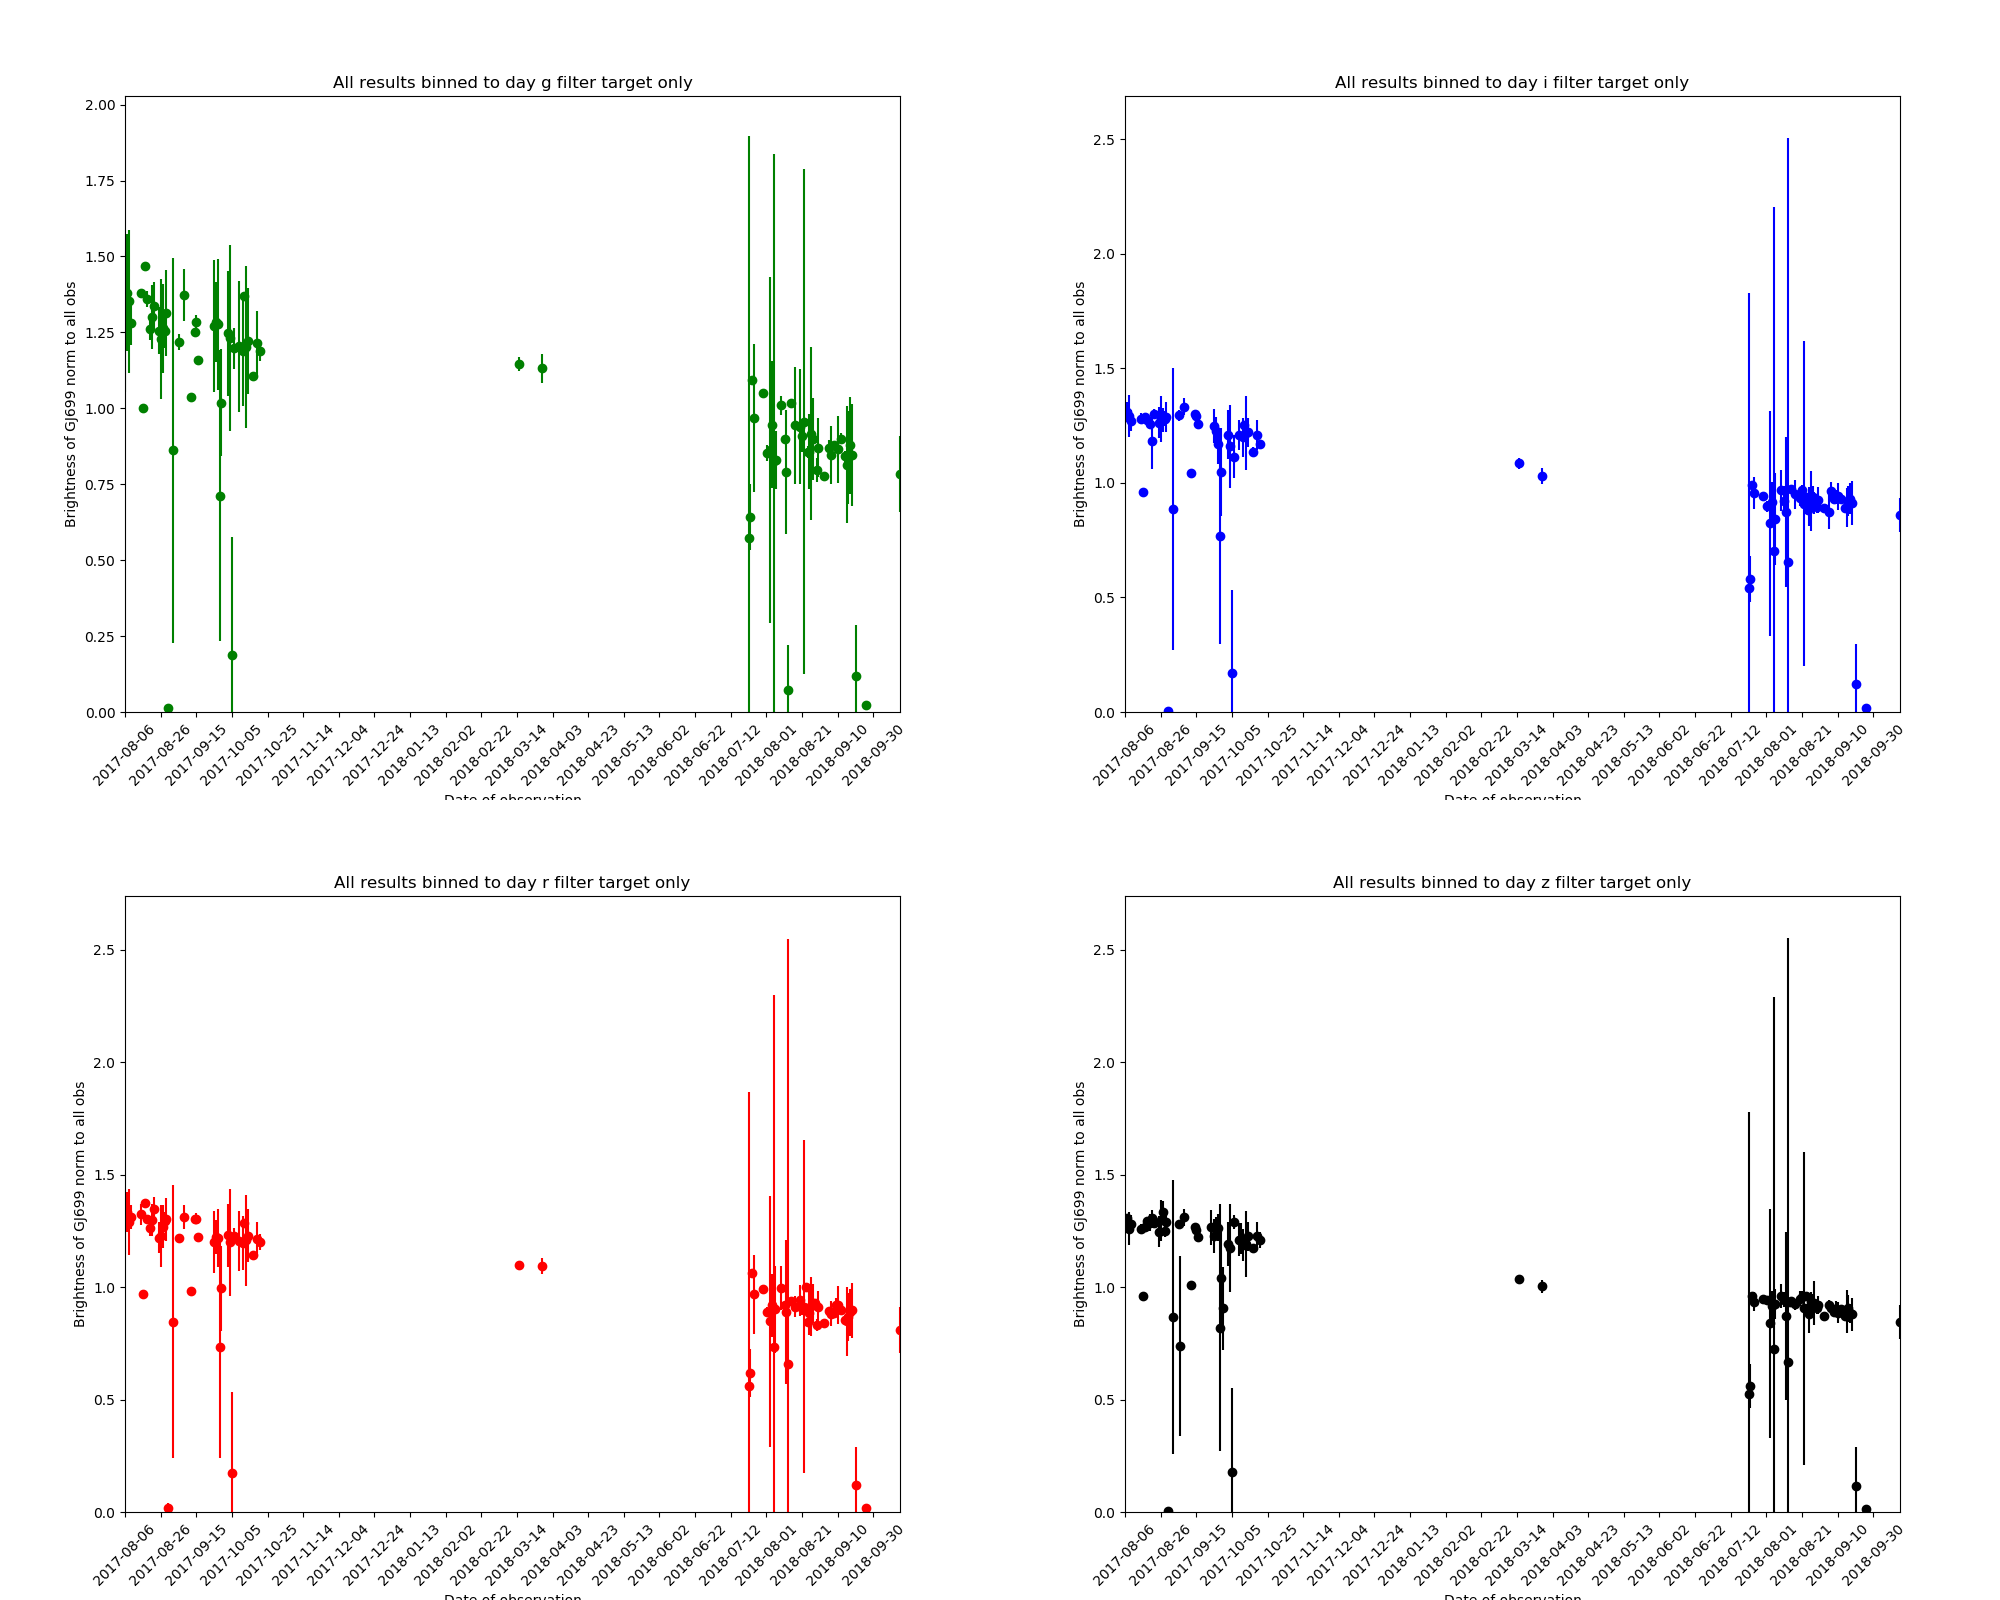
\includegraphics[scale=0.25]{images/allbin.png} \\
% \end{center}   
% \caption{This shows the flux for the target, \bstar, for each of the four visible light filters and binned to a single day. Error bars are show to indicate the spread of intensities over a single day.}
%   \protect\label{fig:allbin}
% \end{figure}

%\begin{figure}[!htbp]
%\begin{center}
%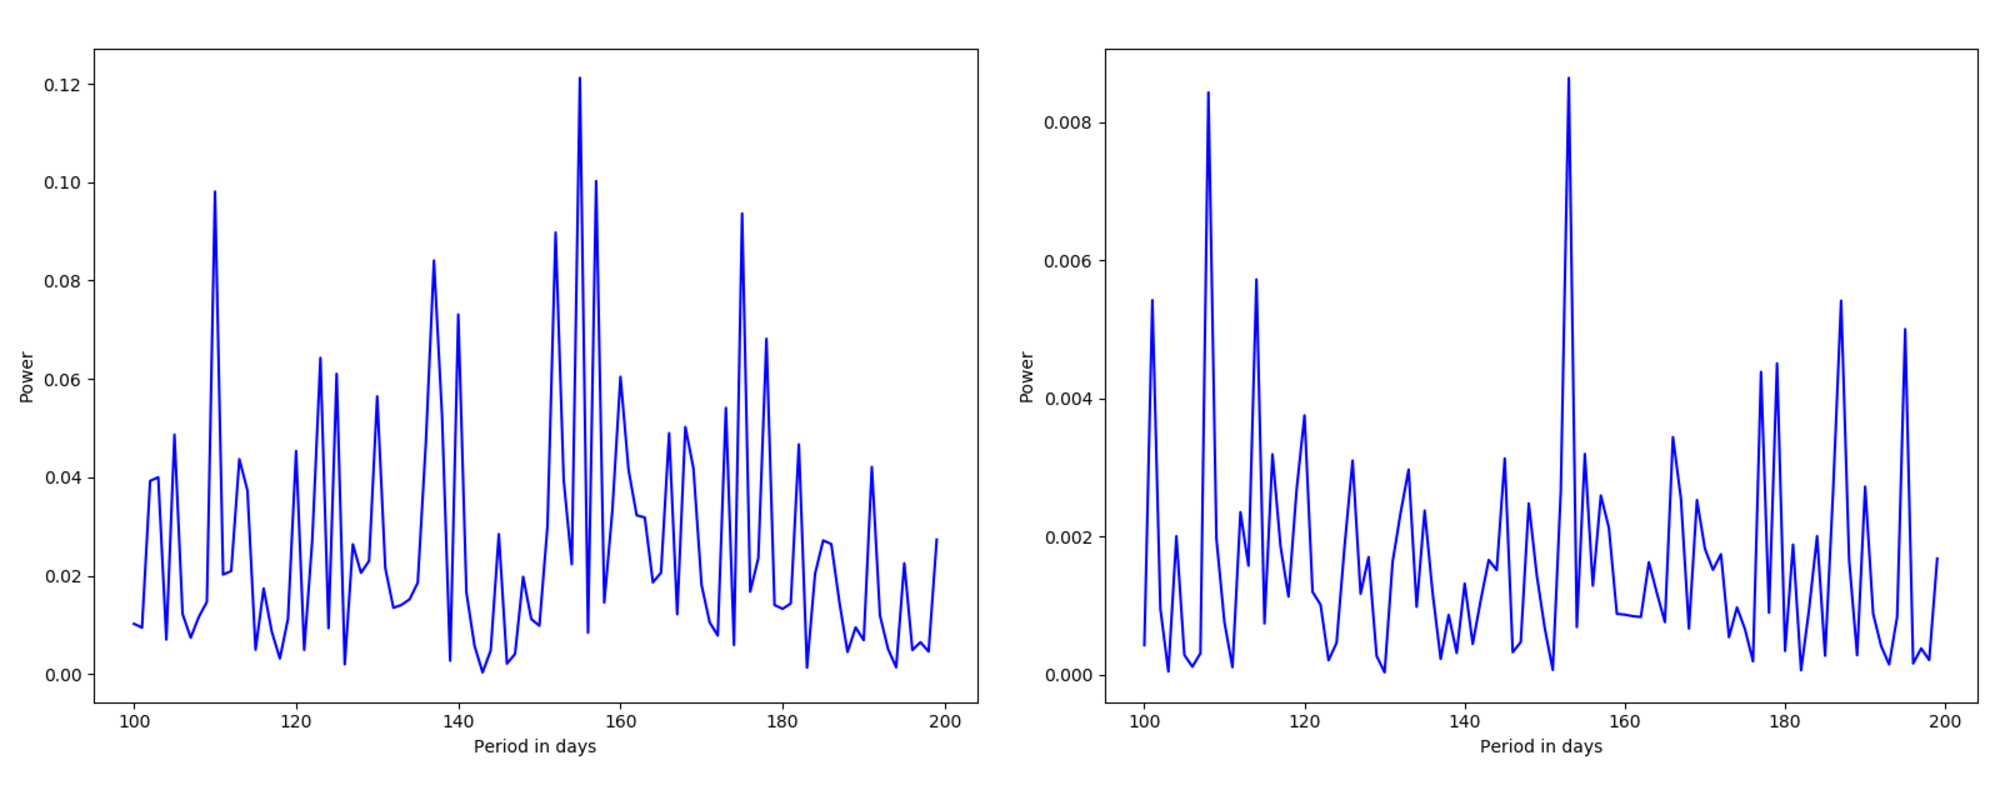
\includegraphics[scale=0.25]{images/pgrambunb.png} \\
%\end{center}   
%\caption{This displays periodograms derived from the binned (Fig.
% \ref{fig:allbin}) and unbinned (Fig. \ref{fig:allall}) light curves for the \textbf{r} filter.}
%  \protect\label{fig:pgrams}
%\end{figure}

% It is accepted that this initial treatment is crude. Serious work needs to be done on correction for air mass,
% which for a few observations, where they are spread over a period of several hours,
% can be quite large, and to more accurately discard as unacceptable images with large or very variable sky levels.
% There are some currently inexplicable variations, for
% example the to images in Fig. \ref{fig:tyeg} give radically different ADU counts despite being taken two minutes apart
% with same exposure time and other parameters.
% 
% \begin{figure}[!htbp]
% \begin{center}
% 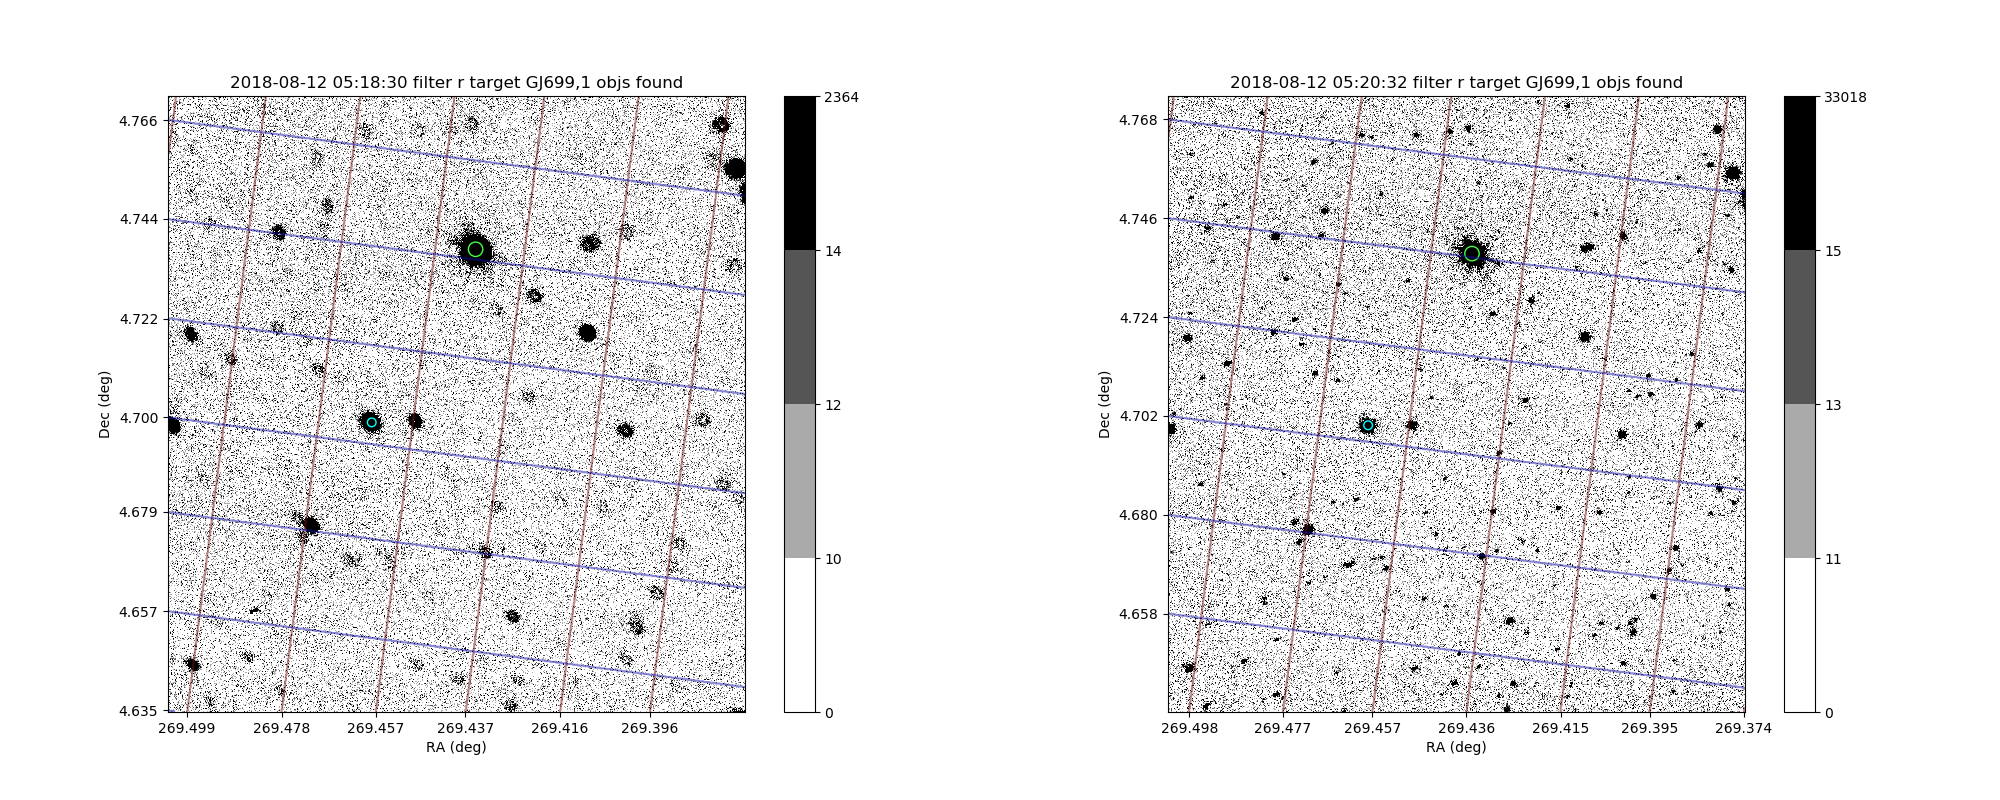
\includegraphics[scale=0.25]{images/tyeg.png}
% \end{center}   
% \caption{These images show an example of where 2 images taken 2 minutes apart with the same exposure time gave different flux values.}
%   \protect\label{fig:tyeg}
% \end{figure}
% 
% \subsubsection{Reference Stars}
% \protect\label{section:refstars}
% 
% Rather than relying on the ``raw'' flux from the target star itself, it was
% considered that an approach based on identified reference stars found in a
% significant number of images.
% Ideally these should be as many as possible to ``smooth'' out errors and variations on the reference star. 
% Byy taking the ratio of the target star ADU count to the sum of the reference
% star ADUs, then we can hope to achieve results for intensity with the factors such air mass corrections factored out, This
% approach was taken in \citet{berry11} and would seem to involve least work, provided sufficient reference stars are
% consistently found.
% 
% The algoritm used to find objects was first to locate the target (there was
% usually a certain amount of error in the coordinates of the images) and then
% find prefeviously-known reference objects. The criterion for finding objects was to look for groups of pixels within a
% given scan aperture whose mean count was a given number of standard deviations
% (intially 3) from that of the sky level. If the result appeared to be one of
% the objects known already, the given reference object was deemed to have been
% found.

% In all cases the brightest objects were found in Simbad, 2MASS and SDSS
% to find objects in the vicinity of \bstar, obtaining the following stars as shown in Table \ref{table:reftimesfound}.
% Of the stars there, the types are unavailable apart from the most-frequently occurring one of
% TYC425-262-1, which is an A3V star (this is also reported as the most frequently found reference star in \citet{berry11}).
% 
% \begin{table}[!htbp]
% \begin{center}
% \begin{tabular}{llr} \hline
% Number & Object & Times found \\\hline
% 1 & TYC425-262-1 & 5,277 \\
% 2 & SDSS1237671695527248969 & 3,408 \\
% 3 & 2MASSJ17574653+0447466 & 3,297 \\
% 4 & SDSS1237668573088841773 & 840 \\
% 5 & TYC425-223-1 & 369 \\
% 6 & SDSS1237671695527249415 & 15 \\
% \hline
% \end{tabular}
% \end{center}
% \caption{This lists the identified reference objects near to {\bstar} and the number of times found in the available
%   data. Note that this data relates to images up to the end of October 2018.}
% \protect\label{table:reftimesfound}
% \end{table}
% 
% I decided to consider only the first 3 reference objects, which are labelled 1, 2 and 3 for convenience in the
% remainder of this report, as the appearances of the others were too infrequent to render them worthwhile.
% 
% \subsection{Classification of results}
% \protect\label{section:classresults}
% 
% The images presented challenges in various respects. The visible light images are all at different orientations and with
% the target in different places in the image, so not all the reference stars appear in all of the images. In some cases
% the reference stars are just not bright enough to rise sufficiently above the sky level.
% 
% \begin{table}[!htbp]
% \begin{center}
% \begin{tabular}{lrrrr}
% &Filter g&Filter i&Filter r&Filter z\\\hline
% Target not found&167&80&105&0\\
% No ref objs found & 84 & 1,003 & 53 & 1,085 \\\hline
% Obj 1 (with or without others) & 834 & 0 & 925 & 0 \\
% Obj 2 (with or without others) & 561 & 1 & 574 & 0 \\
% Obj 3 (with or without others& 526 & 0 & 573 & 0 \\
% Obj 1 only & 43 & 0 & 100 & 0 \\
% Obj 2 only & 0 & 1 & 1 & 0 \\
% Obj 3 only & 0 & 0 & 0 & 0 \\
% Objs 1 and 2 (with or without 3) & 561 & 0 & 573 & 0 \\
% Objs 1 and 3 (with or without 2) & 526 & 0 & 573 & 0 \\
% Objs 2 and 3 (with or without 1) & 296 & 0 & 321 & 0 \\
% Objs 1 and 2 only & 265 & 0 & 252 & 0 \\
% Objs 1 and 3 only & 230 & 0 & 252 & 0 \\
% Objs 2 and 3 only & 0 & 0 & 0 & 0 \\
% Objs 1,2 and 3 & 296 & 0 & 321 & 0 \\
% \hline
% \end{tabular}
% \end{center}
% \caption{This table shows the occurrences of the 3 main reference objects in each of the observations with or without
%   the others. The infrared images were omitted as no reference objects were found in any of them. Note however the lack
%   of occurrences of reference objects in the \textbf{i} and \textbf{z} filter images.}
% \protect\label{table:occtb}
% \end{table}
% 
% \subsection{Results from reference object comparisons}
% \protect\label{section:refobjres}
% 
% Repeating the light curve plots from Section \ref{section:intcomp}, this time as the ratio of the ADU count of the
% target to the sum of the first three reference objects, Fig.  \ref{fig:allref123} and Fig. \ref{fig:allref123bin} show
% the light curves for the \textbf{r} and \textbf{g} filters. Also shown in Fig. \ref{fig:ls123both} are periodograms
% derived from these light curves. Also shown in Fig \ref{fig:allref1}, Fig. \ref{fig:allref1bin} and Fig. \ref{fig:ls1both}
% are the corresponding results taking into account only the brightest of the reference objects, TYC425-262-1.
% 
% \begin{figure}[!htbp]
% \begin{center}
% 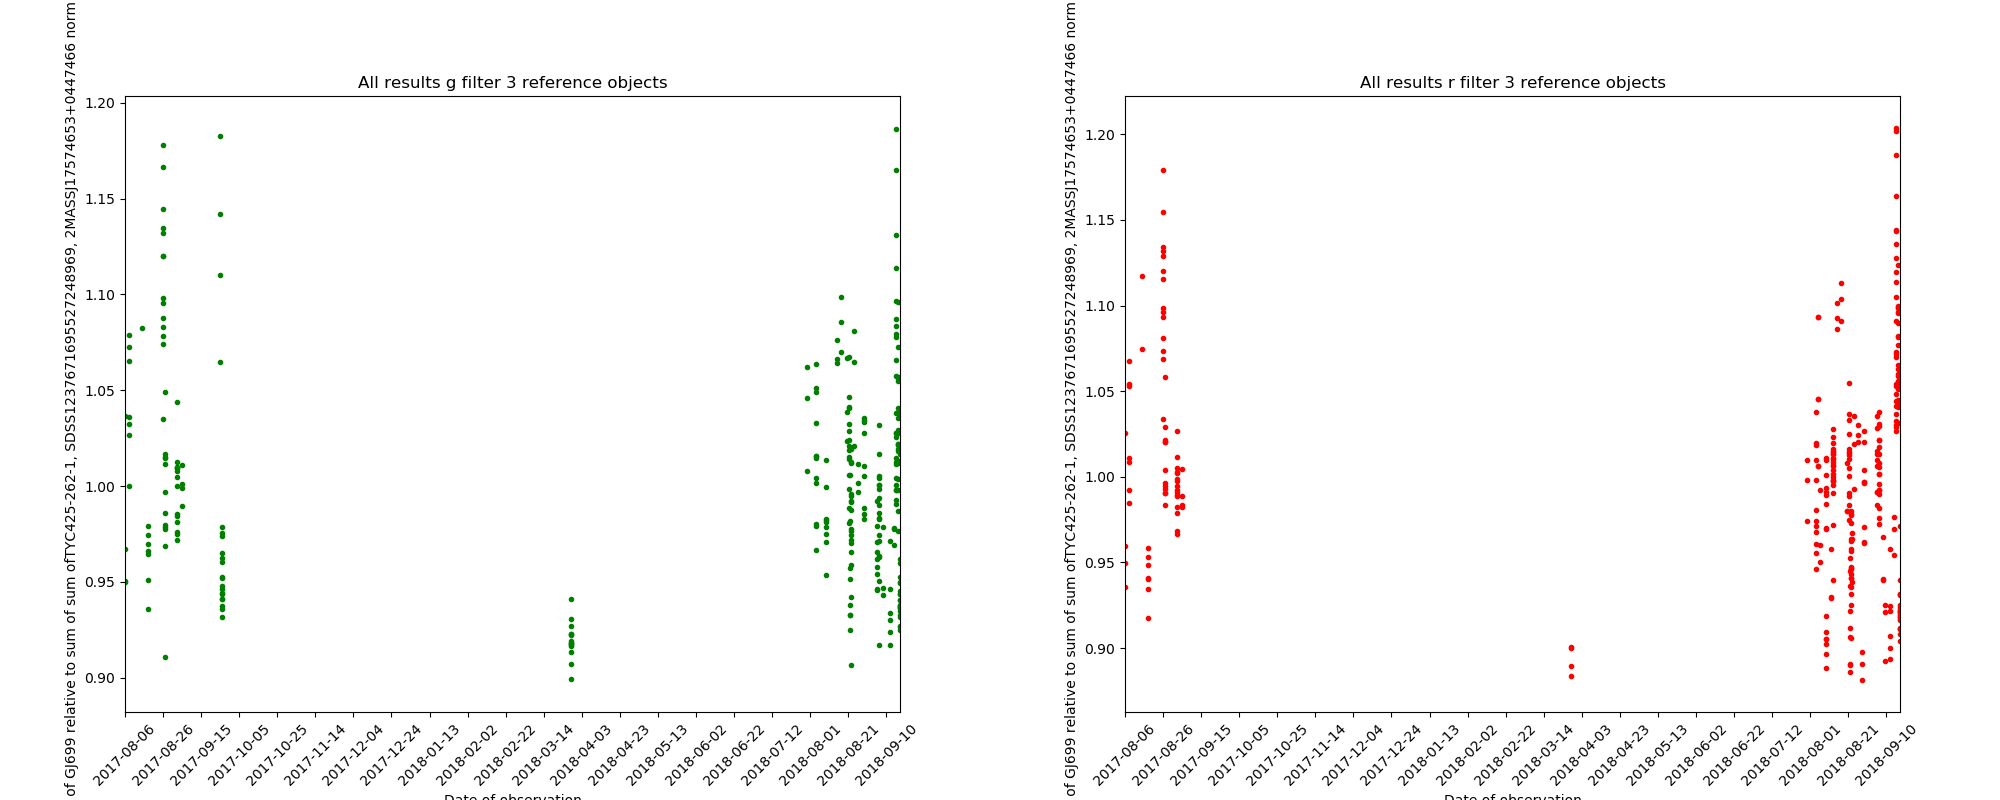
\includegraphics[scale=0.25]{images/allref123.png}
% \end{center}   
% \caption{This shows the ratio of the flux for the target, \bstar, to the 3 main reference objects for the \textbf{g} and
% \textbf{r} filters, plotted as green and red respectively.}
%   \protect\label{fig:allref123}
% \end{figure}
% 
% \begin{figure}[!htbp]
% \begin{center}
% 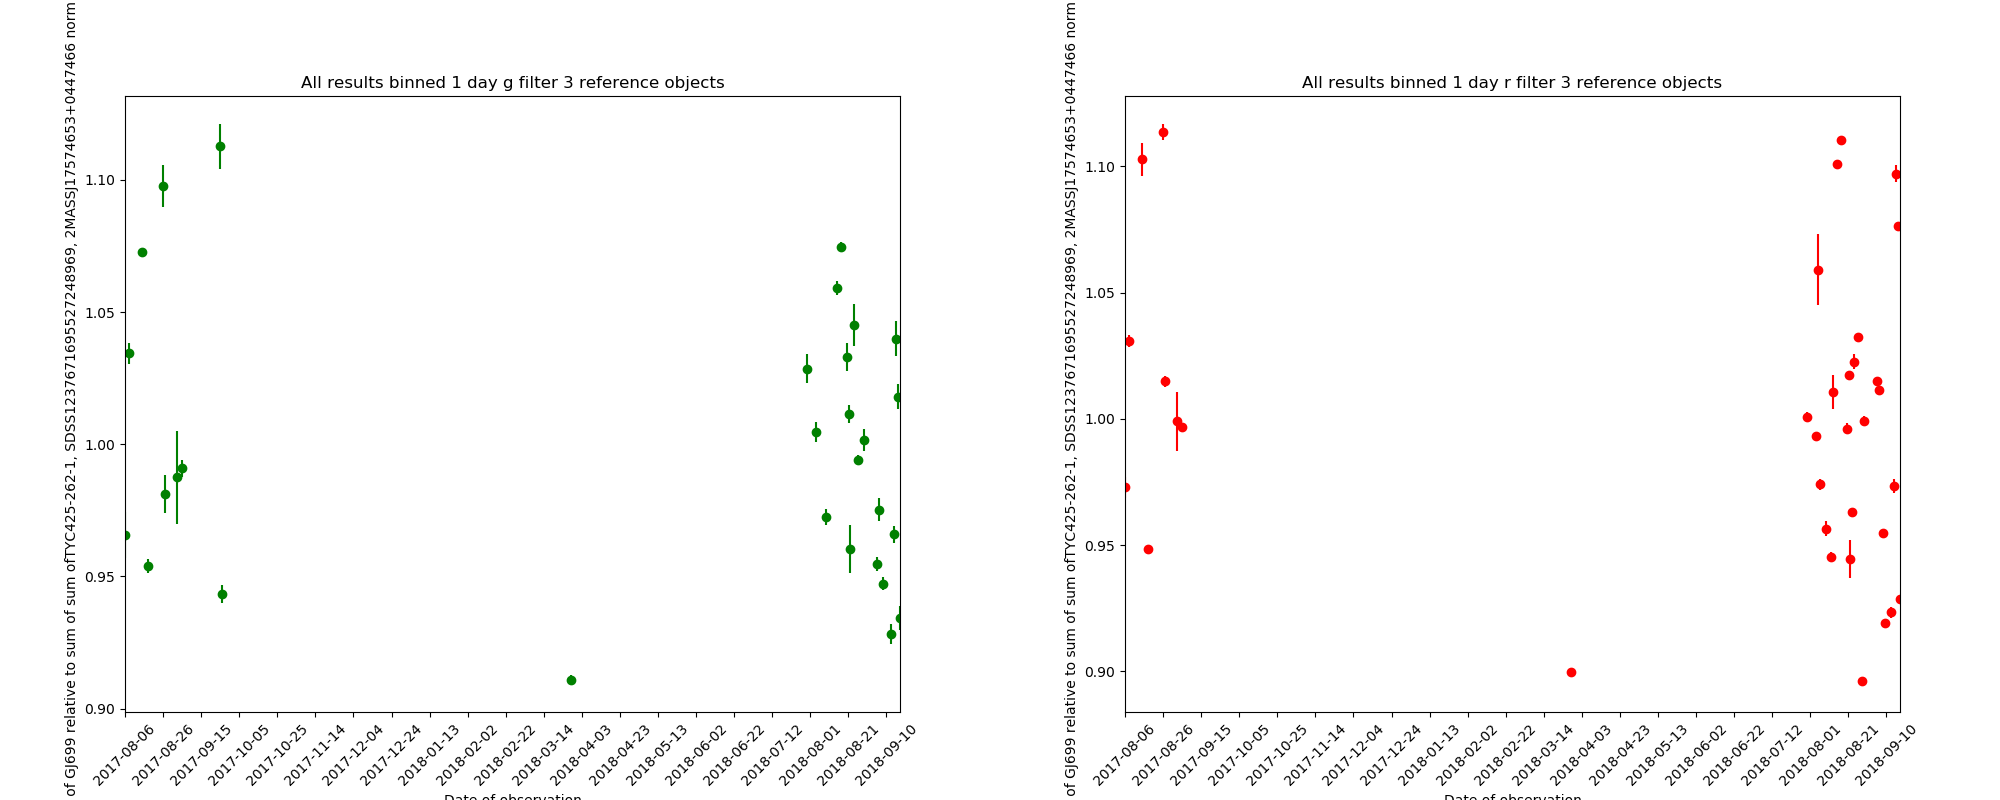
\includegraphics[scale=0.25]{images/allref123bin.png}
% \end{center}   
% \caption{This shows the ratio of the flux for the target, \bstar, to the 3 main reference objects as per Fig. \ref{fig:allref123} and binned to 1 day.}
%   \protect\label{fig:allref123bin}
% \end{figure}
% 
% \begin{figure}[!htbp]
% \begin{center}
% 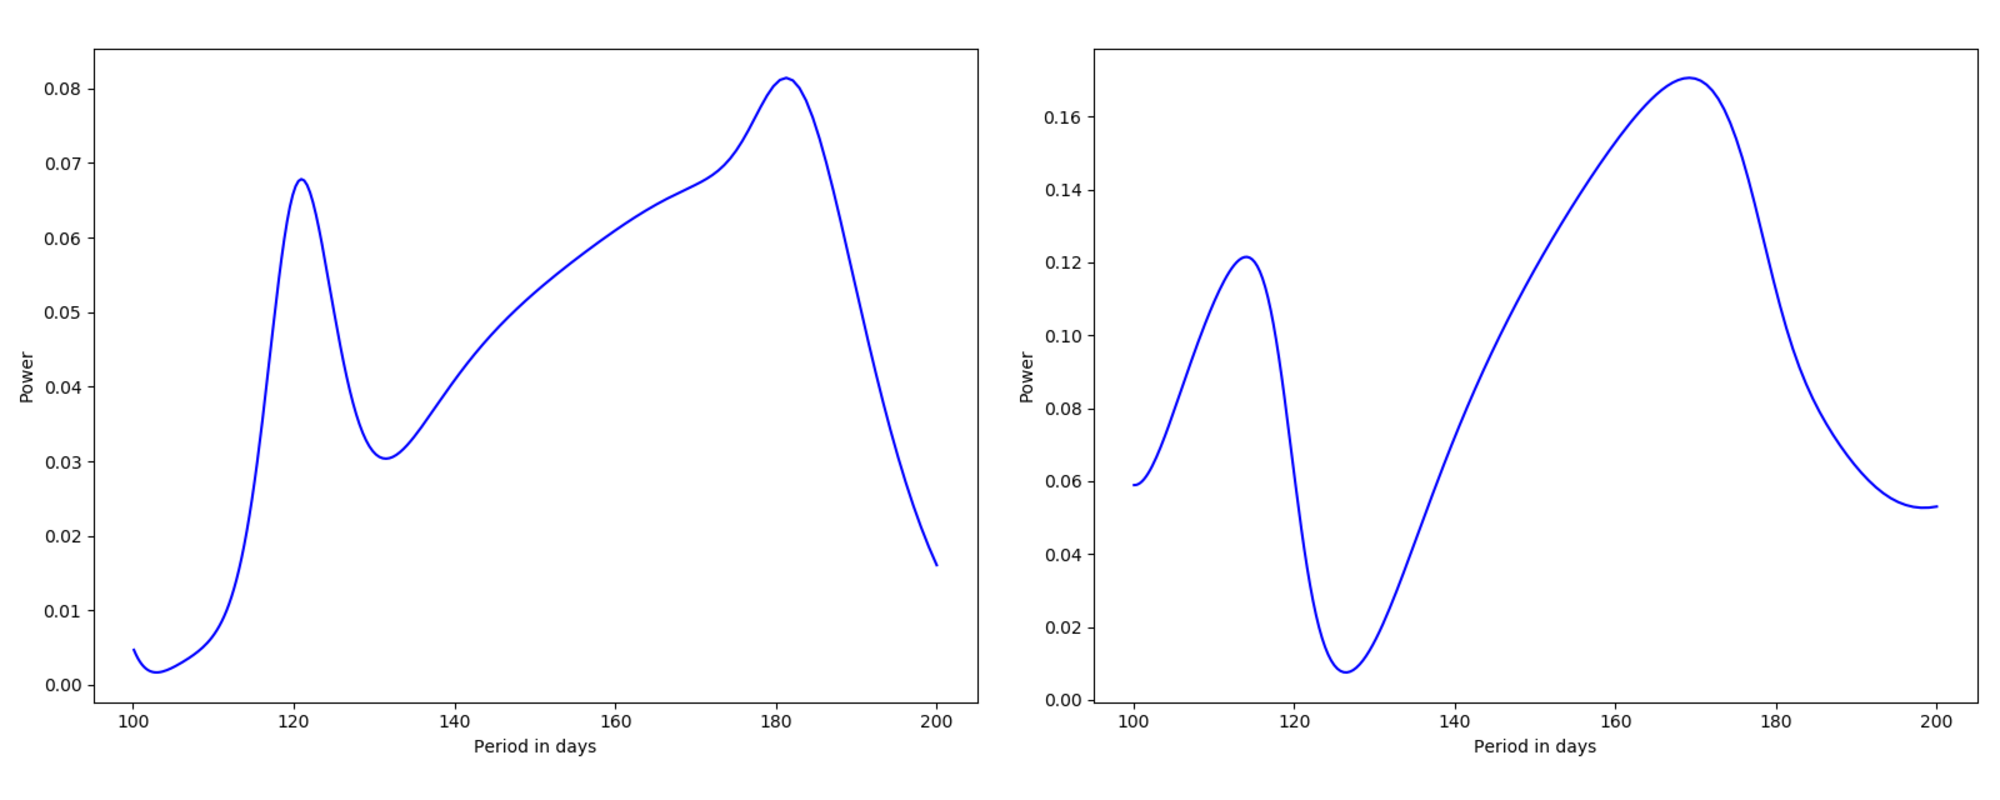
\includegraphics[scale=0.25]{images/ls123both.png}
% \end{center}   
% \caption{Periodograms obtained from Fig. \ref{fig:allref123}, left panel and Fig. \ref{fig:allref123bin} in right
%   panel. Only the \textbf{g} filter was used in this plot, the one from the \textbf{r} filter being almost identical.}
%   \protect\label{fig:ls123both}
% \end{figure}
% 
% \begin{figure}[!htbp]
% \begin{center}
% 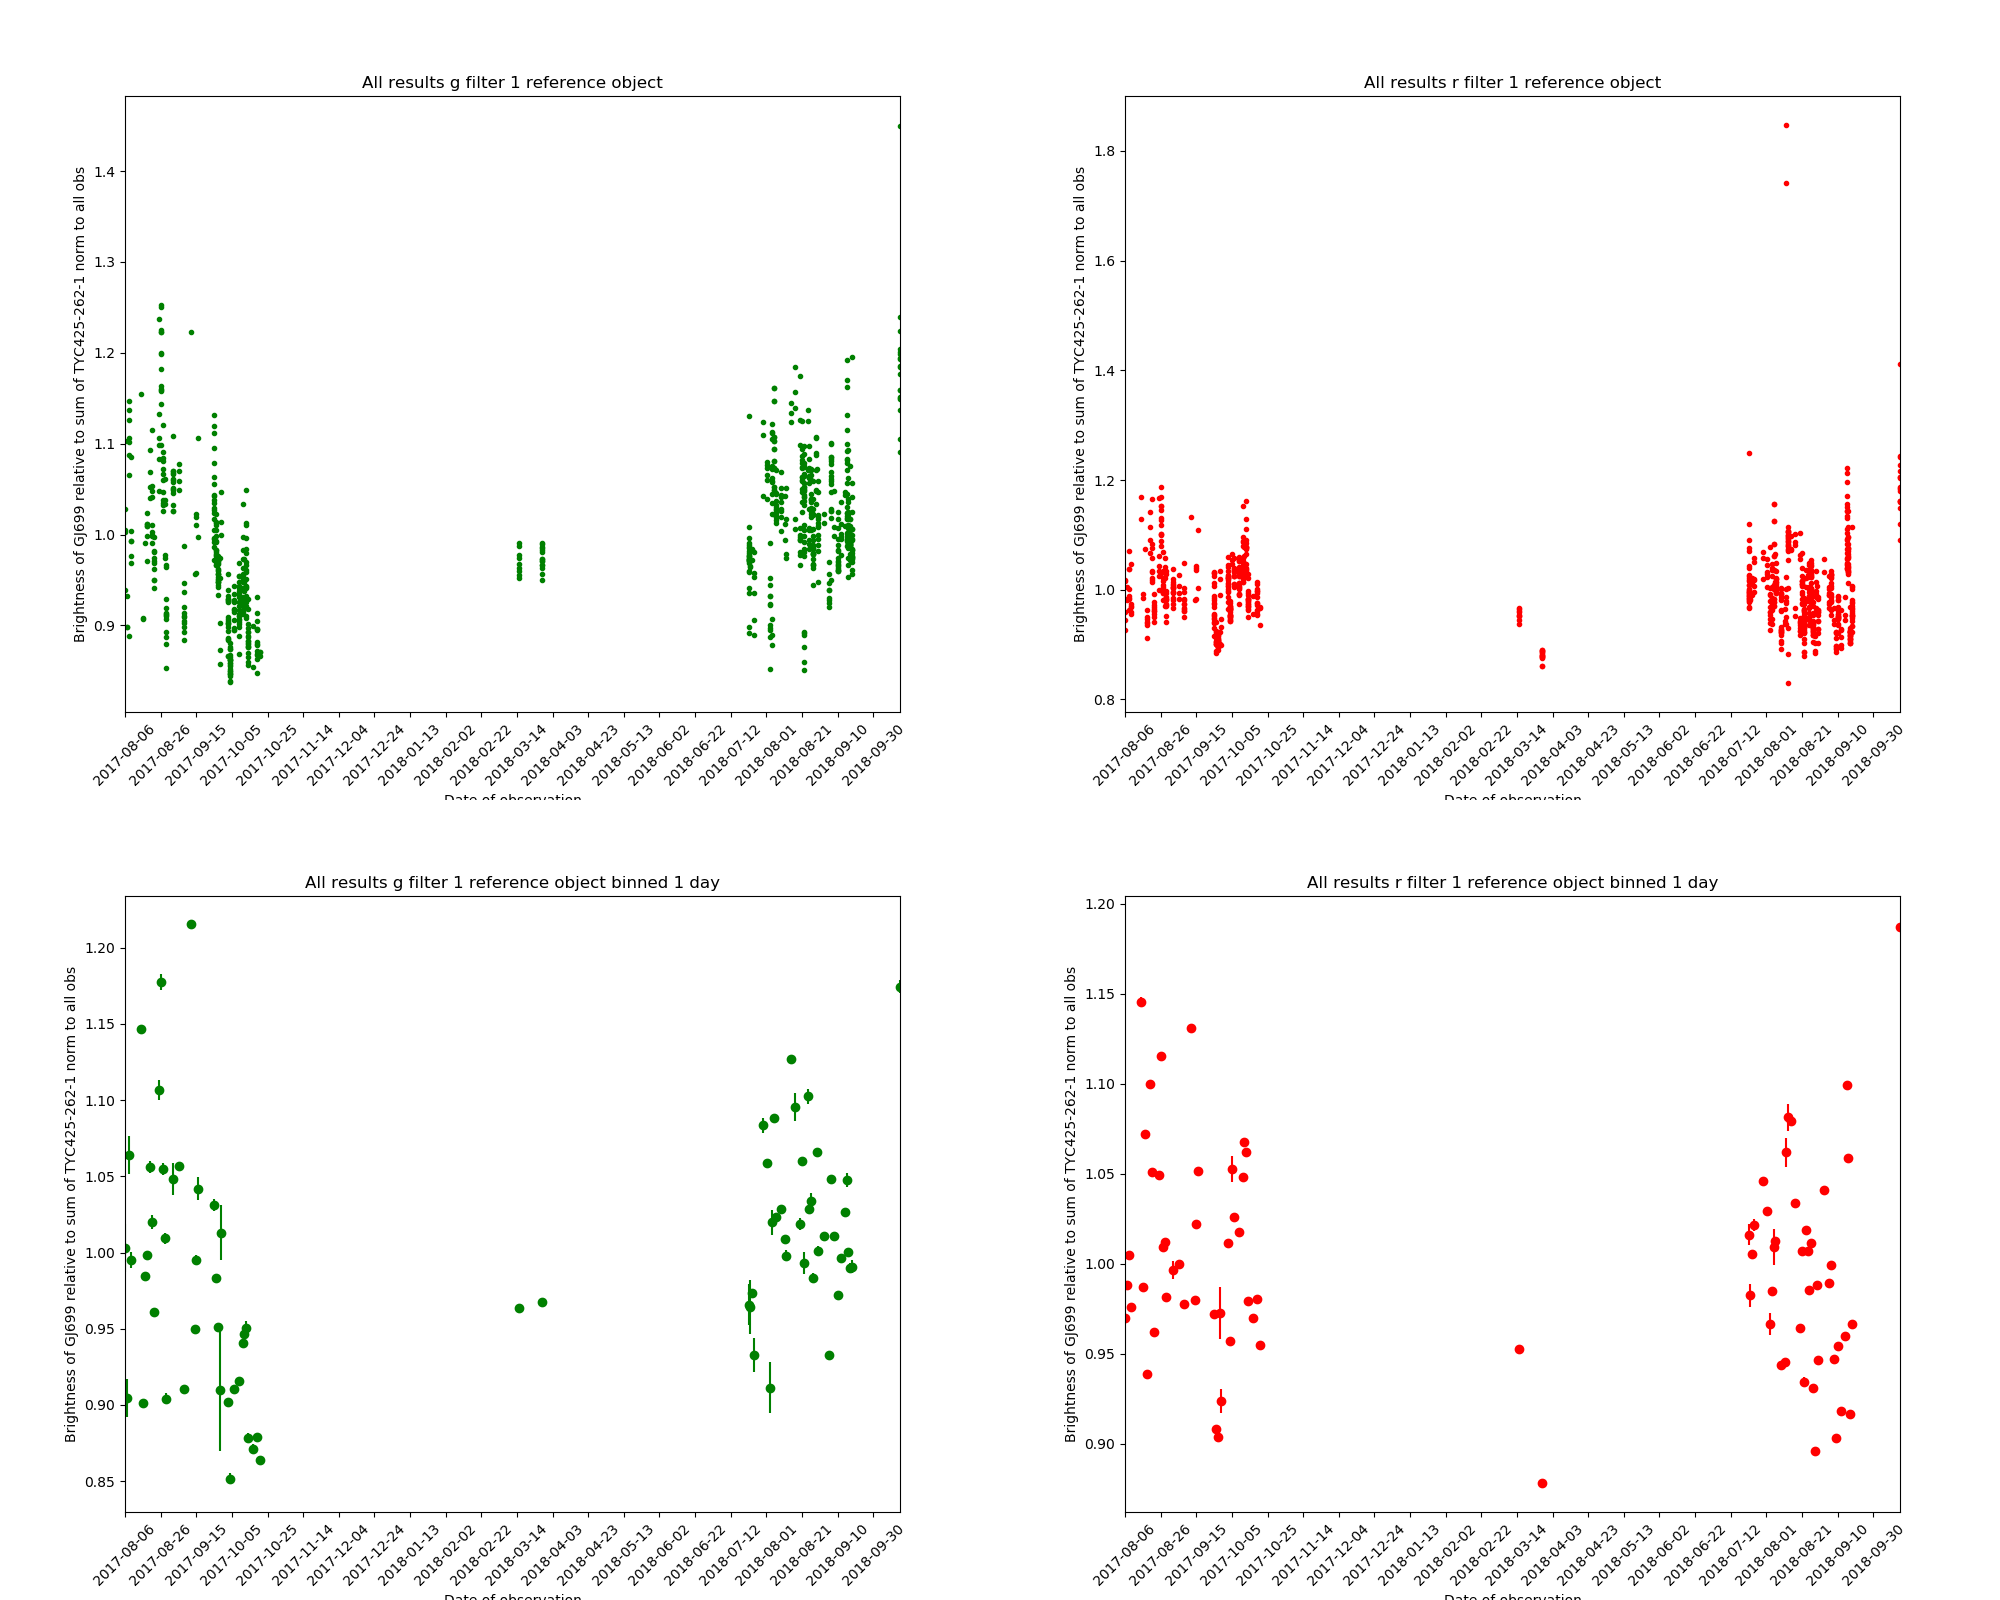
\includegraphics[scale=0.25]{images/allref1.png}
% \end{center}   
% \caption{This shows the ratio of the flux for the target, \bstar, to the strongest of the reference objects, TYC425-262-1.}
%   \protect\label{fig:allref1}
% \end{figure}
% 
% \begin{figure}[!htbp]
% \begin{center}
% 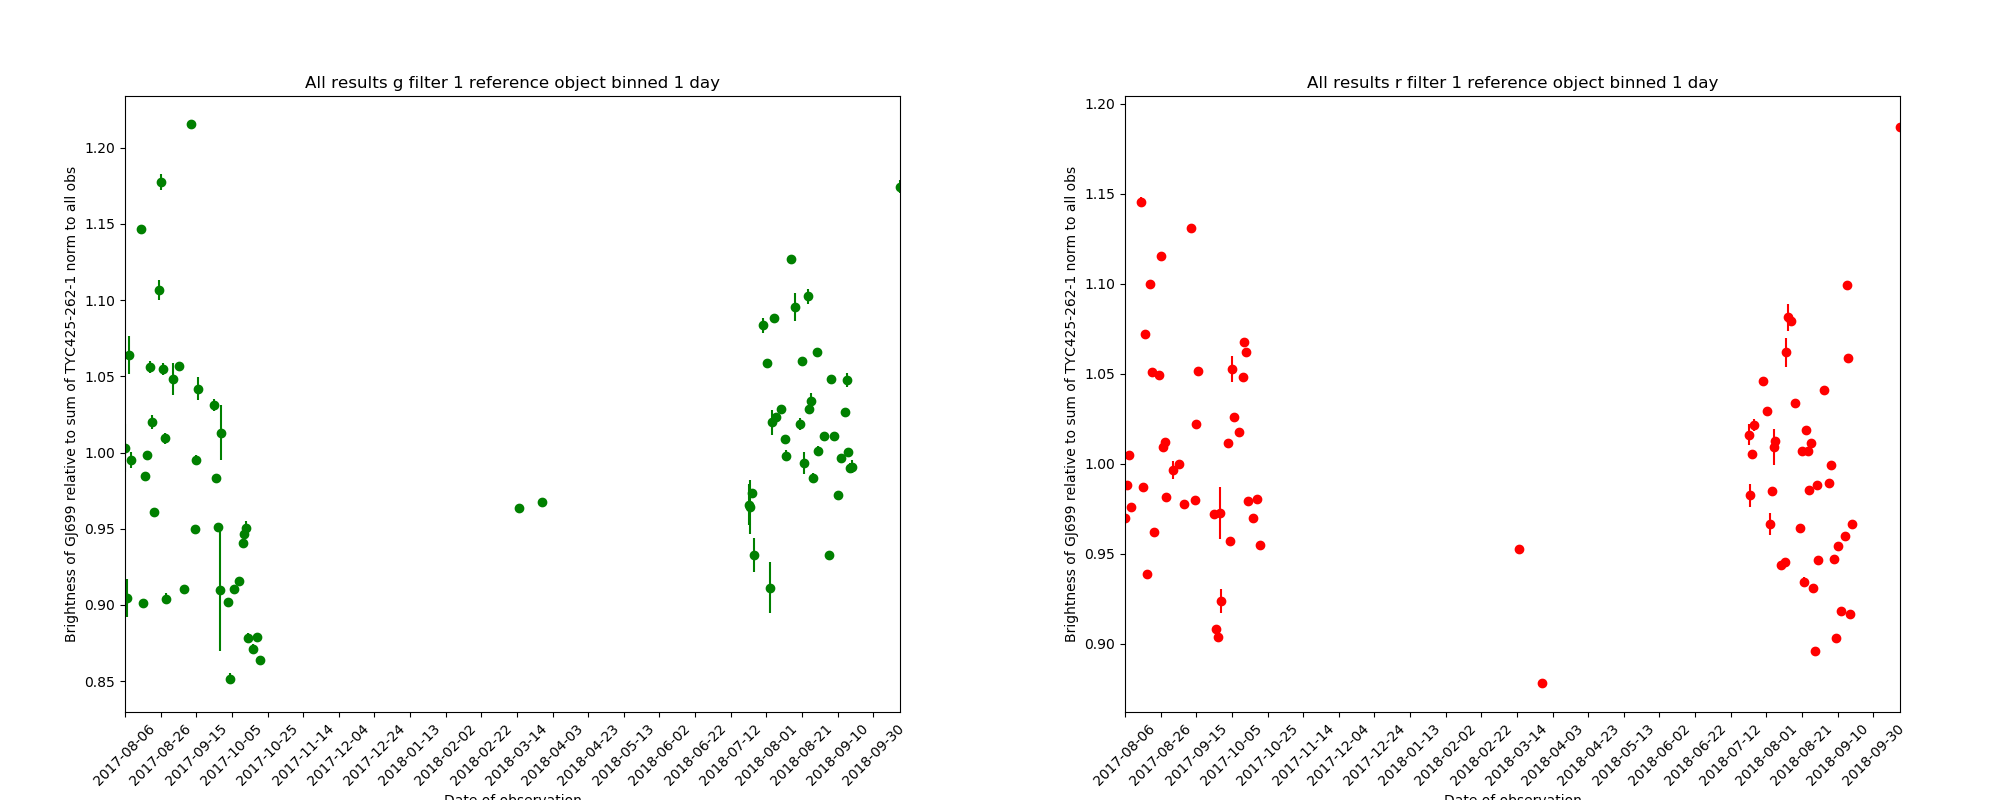
\includegraphics[scale=0.25]{images/allref1bin.png}
% \end{center}   
% \caption{This shows the ratio of the flux for the target, \bstar, to the strongest of the reference objects,
%   TYC425-262-1 per Fig. \ref{fig:allref1} and binned to 1 day.}
%   \protect\label{fig:allref1bin}
% \end{figure}
% 
% \begin{figure}[!htbp]
% \begin{center}
% 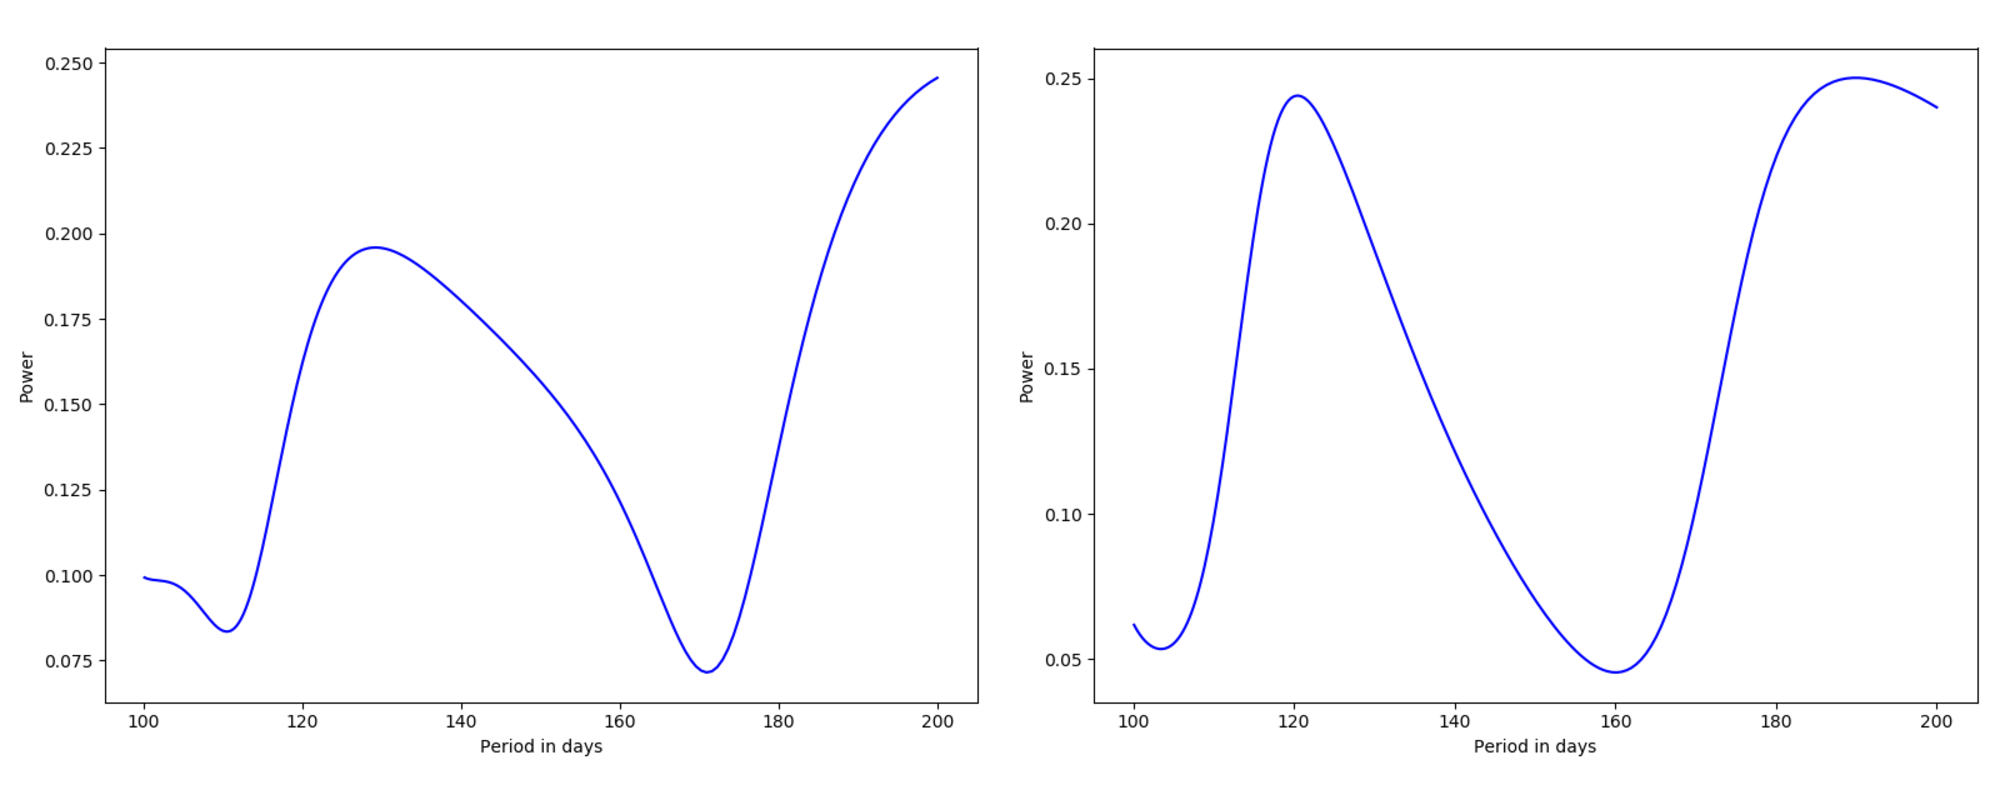
\includegraphics[scale=0.25]{images/ls1both.png}
% \end{center}   
% \caption{Periodograms obtained from Fig. \ref{fig:allref1}, left panel and Fig. \ref{fig:allref1bin} in right
%   panel. Only the \textbf{g} filter was used in this plot, the one from the \textbf{r} filter being almost identical.}
% \protect\label{fig:ls1both}
% \end{figure}
% \clearpage


\section{Processing of data}
\protect\label{section:processing}

In this section the processing of the data on a daily and ongoing basis is
considered.

\subsection{Daily processing}
\protect\label{section:dailyproc}

A daily routine was set up on the Cluster (and in parallel on my home machine)
to do the following.

\begin{enumerate}
  \item Load rows of data corresponding to the observations taken for the
  preceding night.
  \item For the observations of interest, in terms of the targets and for the
  visible light filters, load the corresponding FITS files. Also note parameters
  such as moon phase and distance, exposure time etc.
  \item Load rows of data corresponding to the daily bias and flat files.
  \item Load corresponding FITS files where this is useful (i.e. excluding
  those with a gain of other than 1)
  \item \textit{Not done yet but about to add} note information about
  reliability of each image, assigning a ``quality'' value between 0 and 1.
  Currently this is ``binary'' only but some images, perhaps partly obscured by
  clouds, can still be partly used with a suitable weighting. \textit{I have
  already written the python interface to select images in a given range of
  quality}.
  \item \textit{Not done yet but about to add} do outline find of objects in
  each usable image.
\end{enumerate}

\subsection{Brightness plot of images}
\protect\label{section:recordadus}

After taking each usable image and with the locations of available objects
already found, it is possible to make a light curve for the object over time by
reference to a common subset of reference objects.

Unfortunately due to the differing orientations of the images, the subset of
reference objects is Small the more images are taken. I have set up to be able
to select images by orientation, using 4 different selections may be chosen, 0
representing an orientation with increasing Declination along the Y axis and 1
to 3 respectively selecting an anti-clockwise 90\degree turn from that. This
increases the chances of being able to find a common set of reference objects.
\textit{I need to illustrate this} as does limiting selections to the brightest
overall images.

As discussed in Section \ref{section:fwoptap}, the brightness and variability of
reference objects needs to be established so each frame can be evaluated on the
basis of the reference objects available.

\clearpage
%\section{Method and results}
\protect\label{section:results}

The following approach was taken to analyse the data.

Please note that much of this initial work was done with available data up to
the end of October 2018. There has been later date available in July 2019, but
the images and analysis below were propared before then.

\subsection{Intensity comparison}
\protect\label{section:intcomp}

As a first attempt to study the data, I took the ADU count, specifically the net after applying the flat and bias files
of the target in all the images in which it was available. The target was found in all of the images, apart from in some of the
\textbf{g}, \textbf{i} and \textbf{r} visible light filters, as shown in Table \ref{table:occtb} below.

Plotting light curves of the intensities obtained in this way yields Fig. \ref{fig:allall}.
Binning the intensities together into a single day gave
Fig. \ref{fig:allbin}, the error bars indicate the spread over a single day. I plotted
periodograms, as shown in Fig. \ref{fig:pgrams}. Despite the crudeness of the data, it is noticeable that there are
peaks close to the rotation periods of the order of 150 days referred to in \citet{suarezmascareno15} and \citet{toledopadron18}.

\begin{figure}[!htbp]
\begin{center}
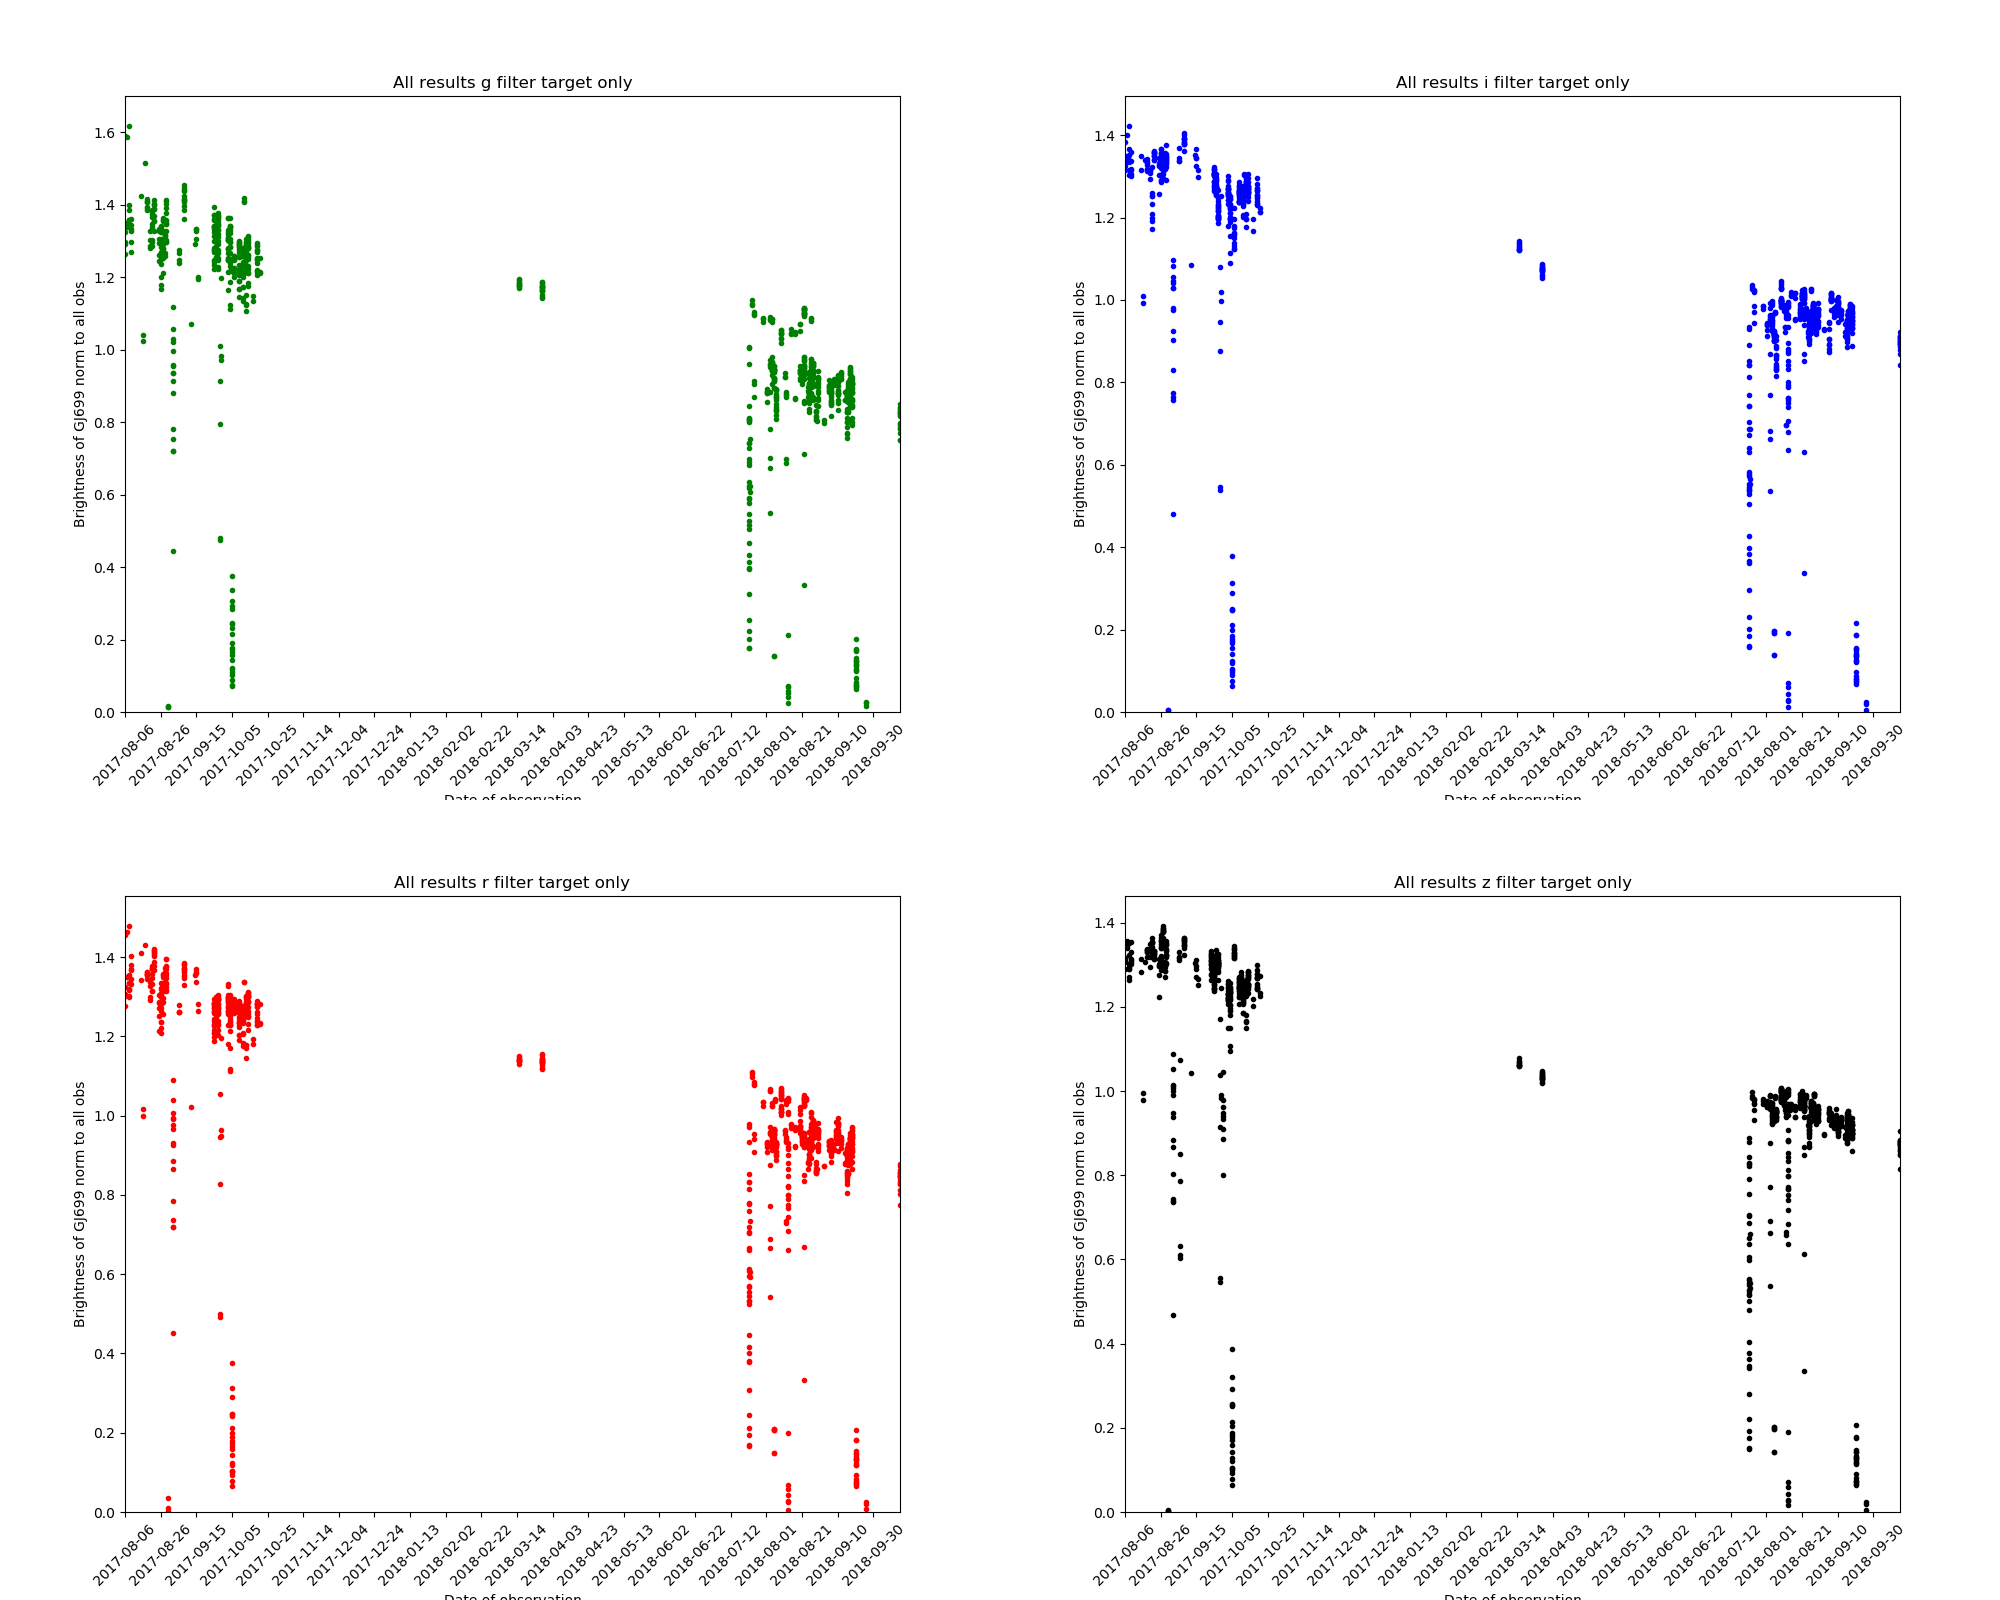
\includegraphics[scale=0.25]{images/allall.png} \\
\end{center}   
\caption{This shows the flux for the target, \bstar, for each of the four visible light filters. This takes the total
  ADU count only}
  \protect\label{fig:allall}
\end{figure}

\begin{figure}[!htbp]
\begin{center}
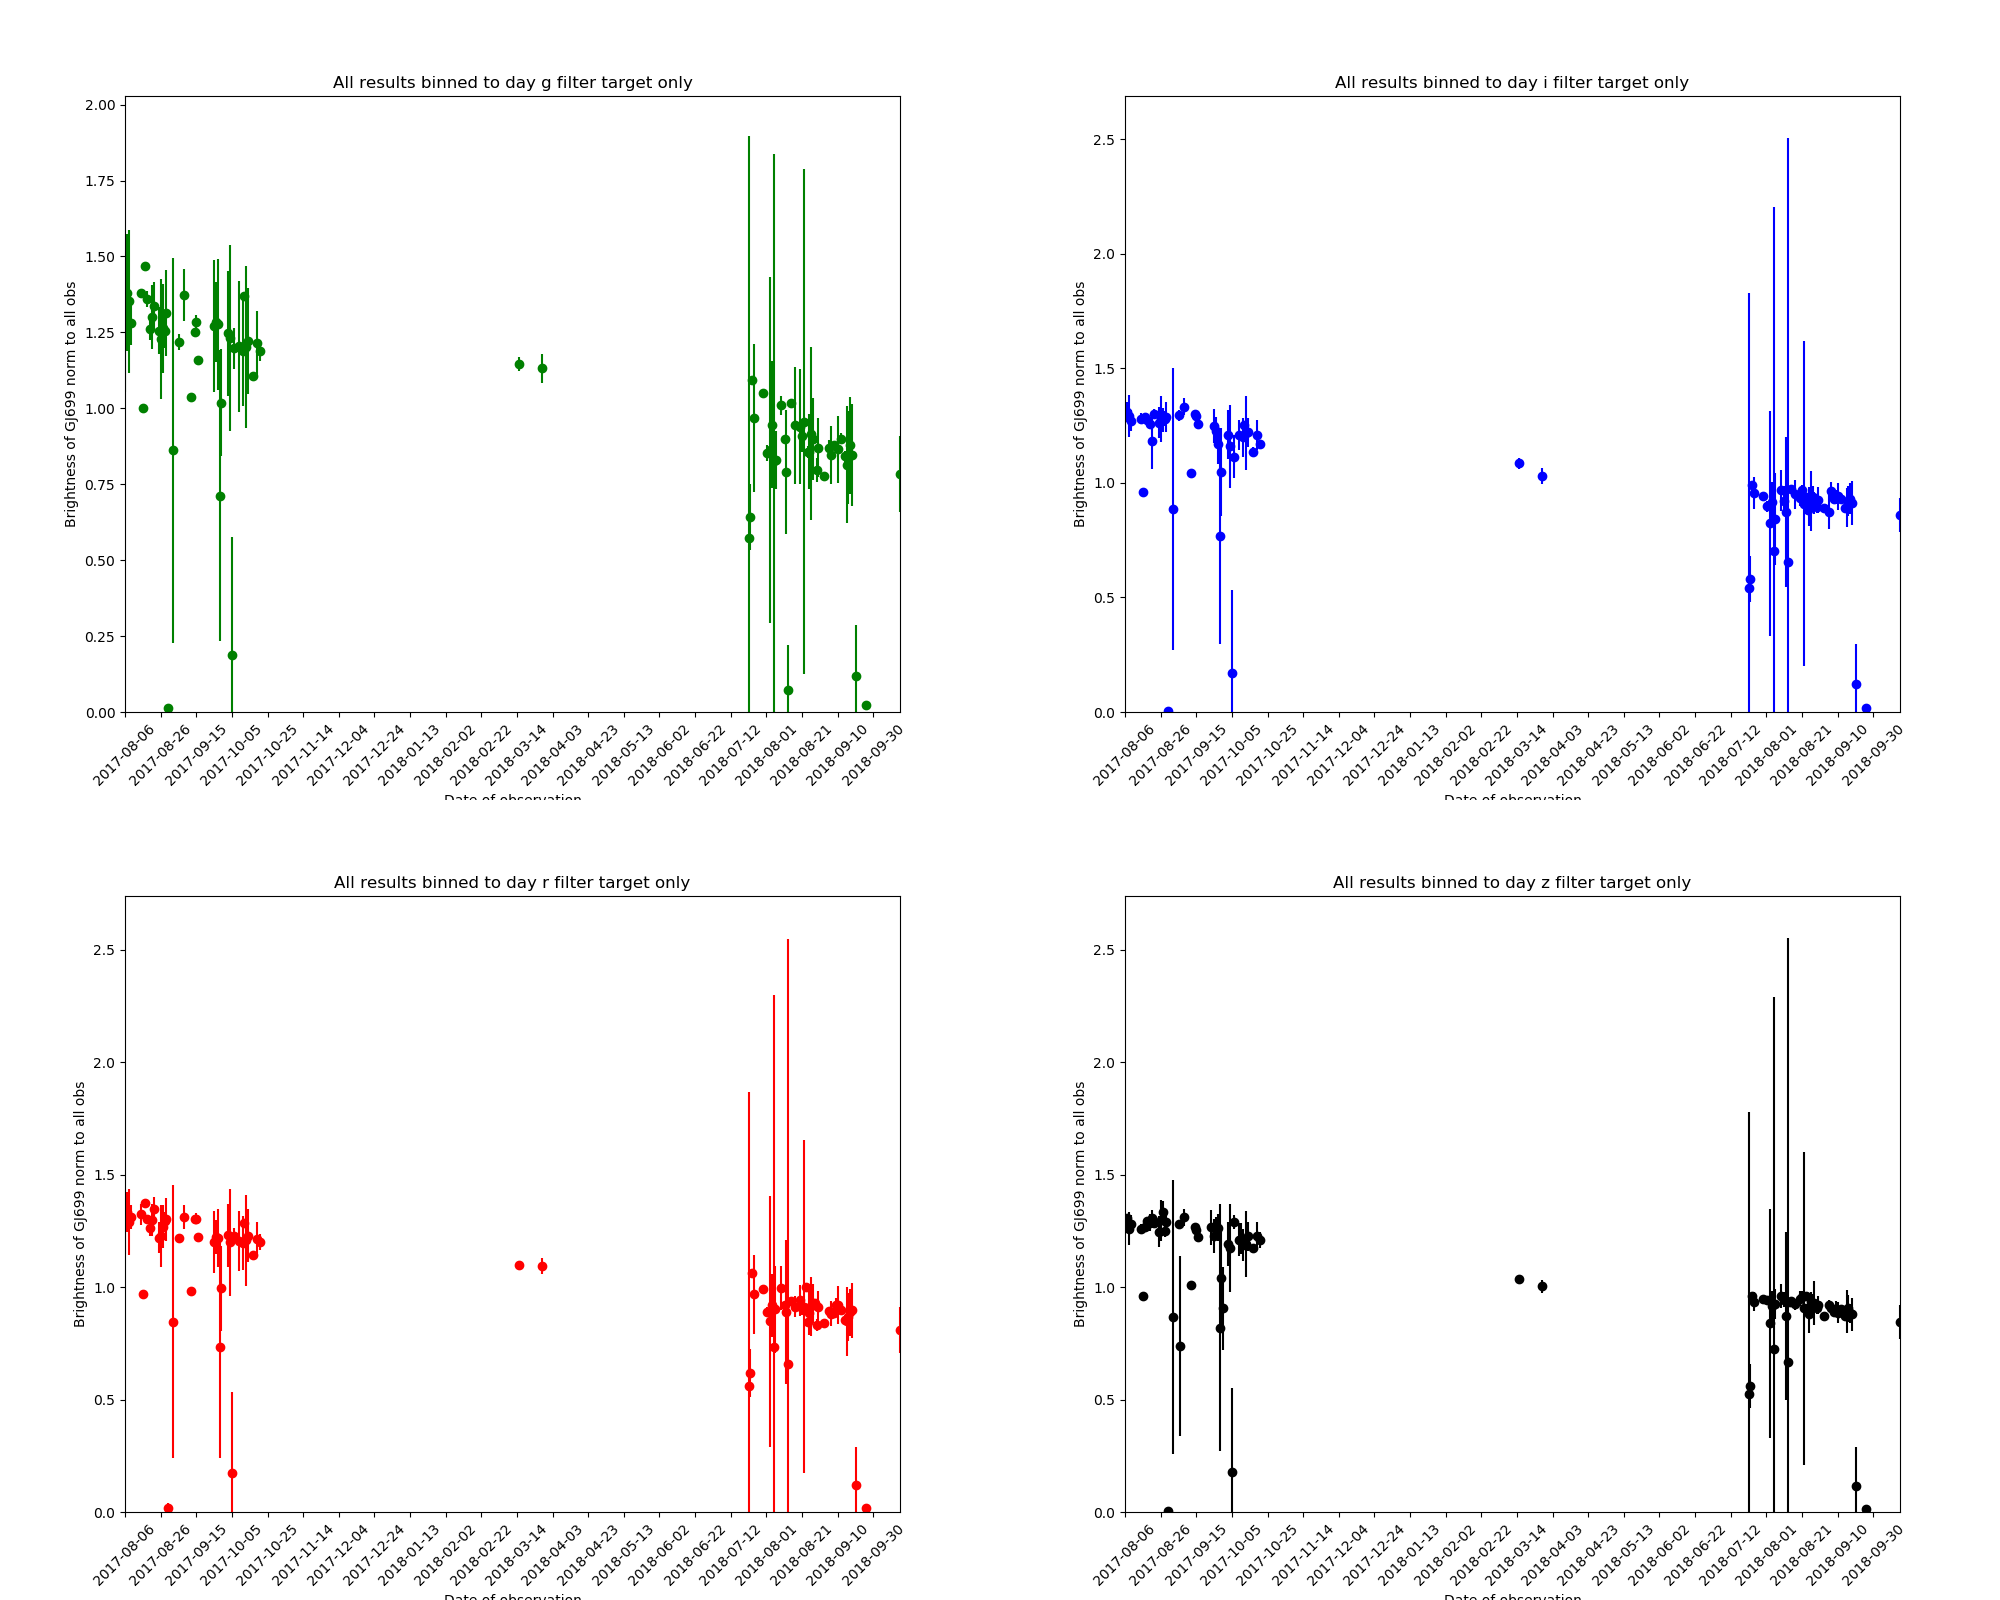
\includegraphics[scale=0.25]{images/allbin.png} \\
\end{center}   
\caption{This shows the flux for the target, \bstar, for each of the four visible light filters and binned to a single day. Error bars are show to indicate the spread of intensities over a single day.}
  \protect\label{fig:allbin}
\end{figure}

\begin{figure}[!htbp]
\begin{center}
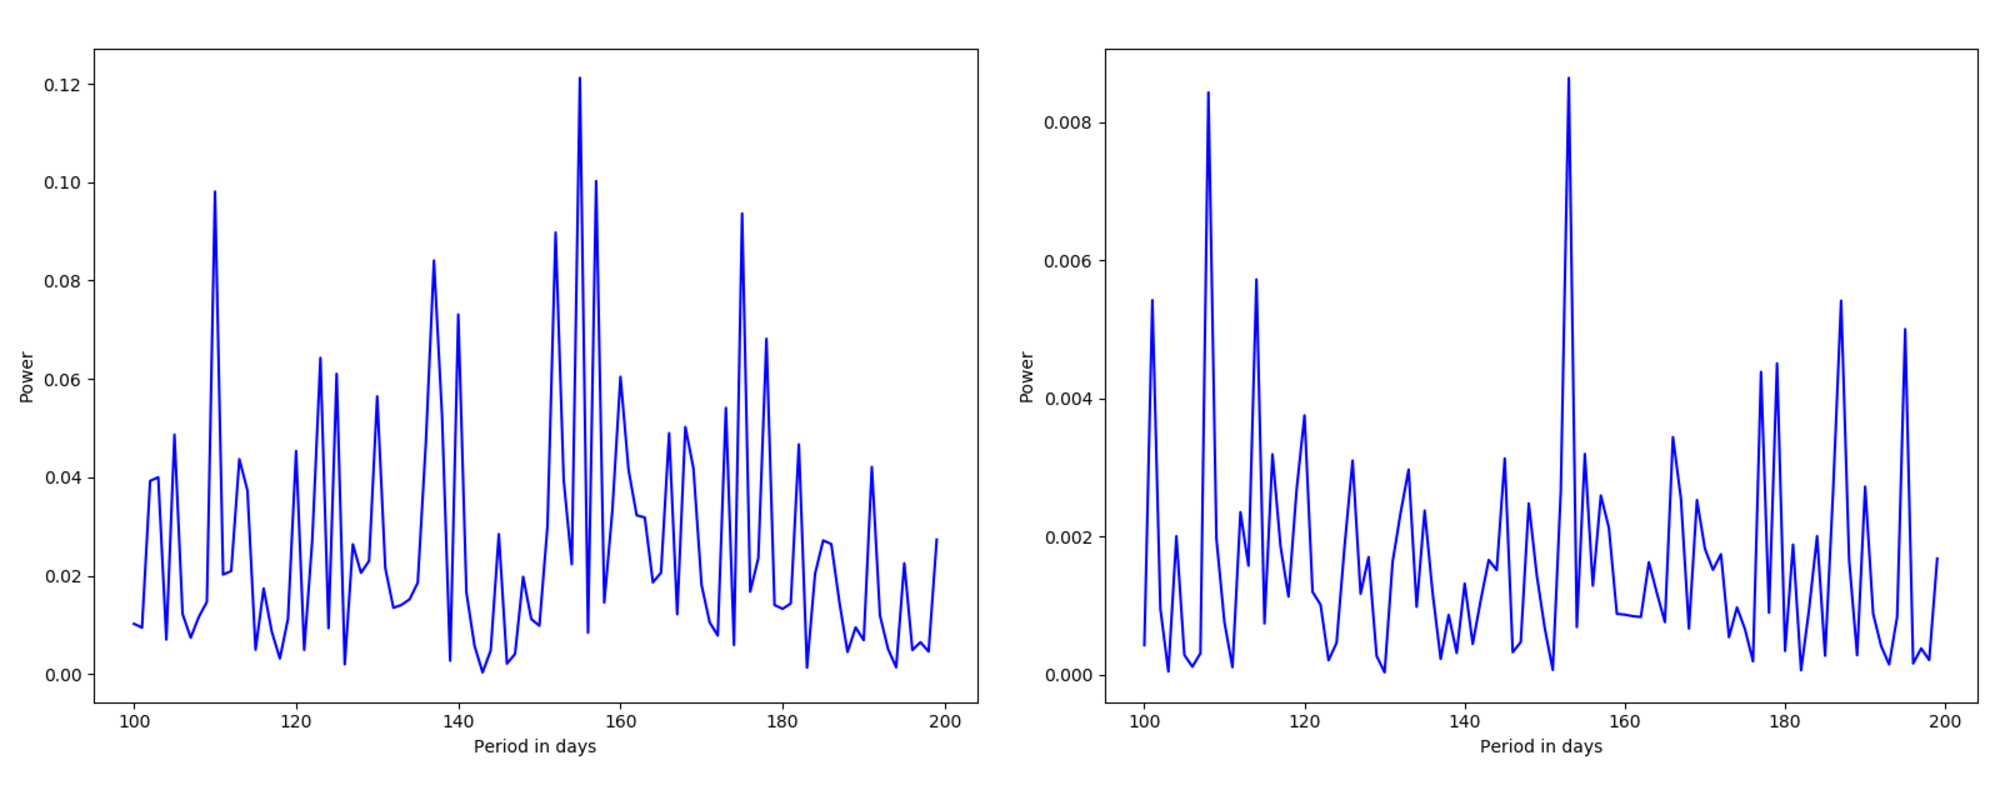
\includegraphics[scale=0.25]{images/pgrambunb.png} \\
\end{center}   
\caption{This displays periodograms derived from the binned (Fig. \ref{fig:allbin}) and unbinned
  (Fig. \ref{fig:allall}) light curves for the \textbf{r} filter.}
  \protect\label{fig:pgrams}
\end{figure}

It is accepted that this initial treatment is crude. Serious work needs to be done on correction for air mass,
which for a few observations, where they are spread over a period of several hours,
can be quite large, and to more accurately discard as unacceptable images with large or very variable sky levels.
There are some currently inexplicable variations, for
example the to images in Fig. \ref{fig:tyeg} give radically different ADU counts despite being taken two minutes apart
with same exposure time and other parameters.

\begin{figure}[!htbp]
\begin{center}
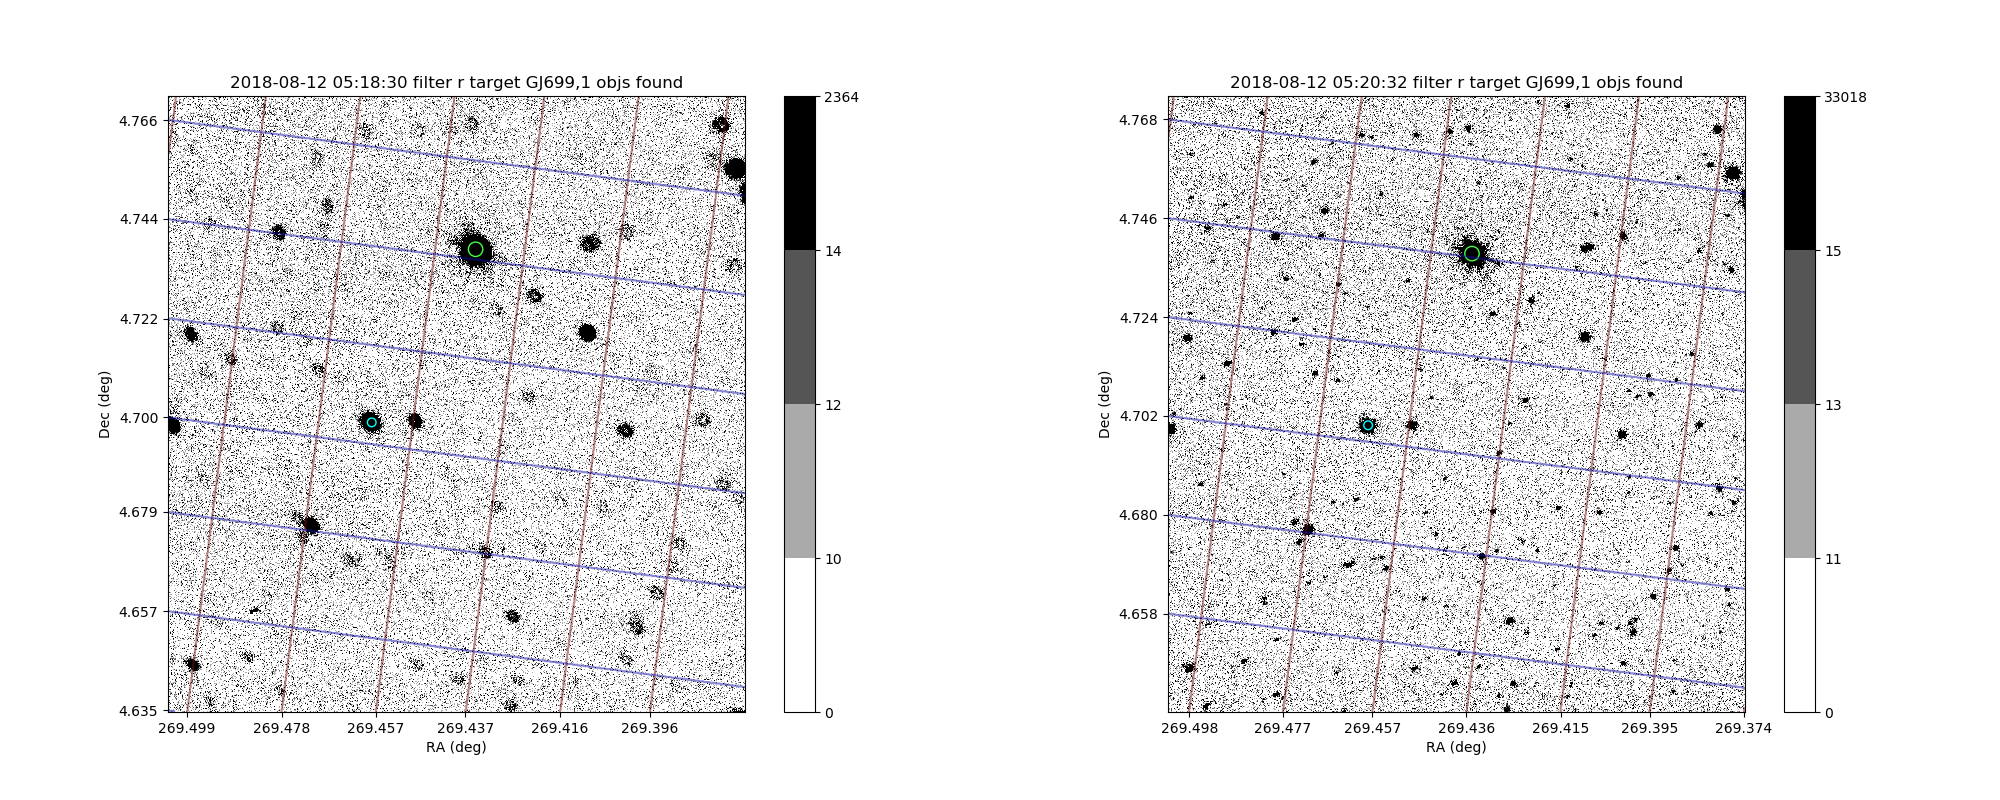
\includegraphics[scale=0.25]{images/tyeg.png}
\end{center}   
\caption{These images show an example of where 2 images taken 2 minutes apart with the same exposure time gave different flux values.}
  \protect\label{fig:tyeg}
\end{figure}

\subsection{Reference Stars}
\protect\label{section:refstars}

Rather than relying on the ``raw'' flux from the target star itself, I made an approach based on identified reference
stars found in a significant number of images. Ideally these should be as many as possible to ``smooth'' out errors and
variations on the reference star. By taking the ratio of the target star ADU count to the sum of the reference star
ADUs, then we can hope to achieve results for intensity with the factors such air mass corrections factored out, This
approach was taken in \citet{berry11} and would seem to involve least work, provided sufficient reference stars are
consistently found.

The algoritm used to find objects was first to locate the target (there was
usually a certain amount of error in the coordinates of the images) and then
find prefeviously-known reference objects. The criterion for finding objects was to look for groups of pixels within a
given scan aperture whose mean count was a given number of standard deviations
(intially 3) from that of the sky level. If the result appeared to be one of
the objects known already, the given reference object was deemed to have been
found.

To initialise the database of objects, I used Simbad, 2MASS and SDSS to find objects in the vicinity of \bstar, obtaining the following stars as shown in Table
\ref{table:reftimesfound}. Of the stars there, the types are unavailable apart from the most-frequently occurring one of
TYC425-262-1, which is an A3V star (this is also reported as the most frequently found reference star in \citet{berry11}).

\begin{table}[!htbp]
\begin{center}
\begin{tabular}{llr} \hline
Number & Object & Times found \\\hline
1 & TYC425-262-1 & 5,277 \\
2 & SDSS1237671695527248969 & 3,408 \\
3 & 2MASSJ17574653+0447466 & 3,297 \\
4 & SDSS1237668573088841773 & 840 \\
5 & TYC425-223-1 & 369 \\
6 & SDSS1237671695527249415 & 15 \\
\hline
\end{tabular}
\end{center}
\caption{This lists the identified reference objects near to {\bstar} and the number of times found in the available
  data. Note that this data relates to images up to the end of October 2018.}
\protect\label{table:reftimesfound}
\end{table}

I decided to consider only the first 3 reference objects, which are labelled 1, 2 and 3 for convenience in the
remainder of this report, as the appearances of the others were too infrequent to render them worthwhile.

\subsection{Classification of results}
\protect\label{section:classresults}

The images presented challenges in various respects. The visible light images are all at different orientations and with
the target in different places in the image, so not all the reference stars appear in all of the images. In some cases
the reference stars are just not bright enough to rise sufficiently above the sky level.

\begin{table}[!htbp]
\begin{center}
\begin{tabular}{lrrrr}
&Filter g&Filter i&Filter r&Filter z\\\hline
Target not found&167&80&105&0\\
No ref objs found & 84 & 1,003 & 53 & 1,085 \\\hline
Obj 1 (with or without others) & 834 & 0 & 925 & 0 \\
Obj 2 (with or without others) & 561 & 1 & 574 & 0 \\
Obj 3 (with or without others& 526 & 0 & 573 & 0 \\
Obj 1 only & 43 & 0 & 100 & 0 \\
Obj 2 only & 0 & 1 & 1 & 0 \\
Obj 3 only & 0 & 0 & 0 & 0 \\
Objs 1 and 2 (with or without 3) & 561 & 0 & 573 & 0 \\
Objs 1 and 3 (with or without 2) & 526 & 0 & 573 & 0 \\
Objs 2 and 3 (with or without 1) & 296 & 0 & 321 & 0 \\
Objs 1 and 2 only & 265 & 0 & 252 & 0 \\
Objs 1 and 3 only & 230 & 0 & 252 & 0 \\
Objs 2 and 3 only & 0 & 0 & 0 & 0 \\
Objs 1,2 and 3 & 296 & 0 & 321 & 0 \\
\hline
\end{tabular}
\end{center}
\caption{This table shows the occurrences of the 3 main reference objects in each of the observations with or without
  the others. The infrared images were omitted as no reference objects were found in any of them. Note however the lack
  of occurrences of reference objects in the \textbf{i} and \textbf{z} filter images.}
\protect\label{table:occtb}
\end{table}

\subsection{Results from reference object comparisons}
\protect\label{section:refobjres}

Repeating the light curve plots from Section \ref{section:intcomp}, this time as the ratio of the ADU count of the
target to the sum of the first three reference objects, Fig.  \ref{fig:allref123} and Fig. \ref{fig:allref123bin} show
the light curves for the \textbf{r} and \textbf{g} filters. Also shown in Fig. \ref{fig:ls123both} are periodograms
derived from these light curves. Also shown in Fig \ref{fig:allref1}, Fig. \ref{fig:allref1bin} and Fig. \ref{fig:ls1both}
are the corresponding results taking into account only the brightest of the reference objects, TYC425-262-1.

\begin{figure}[!htbp]
\begin{center}
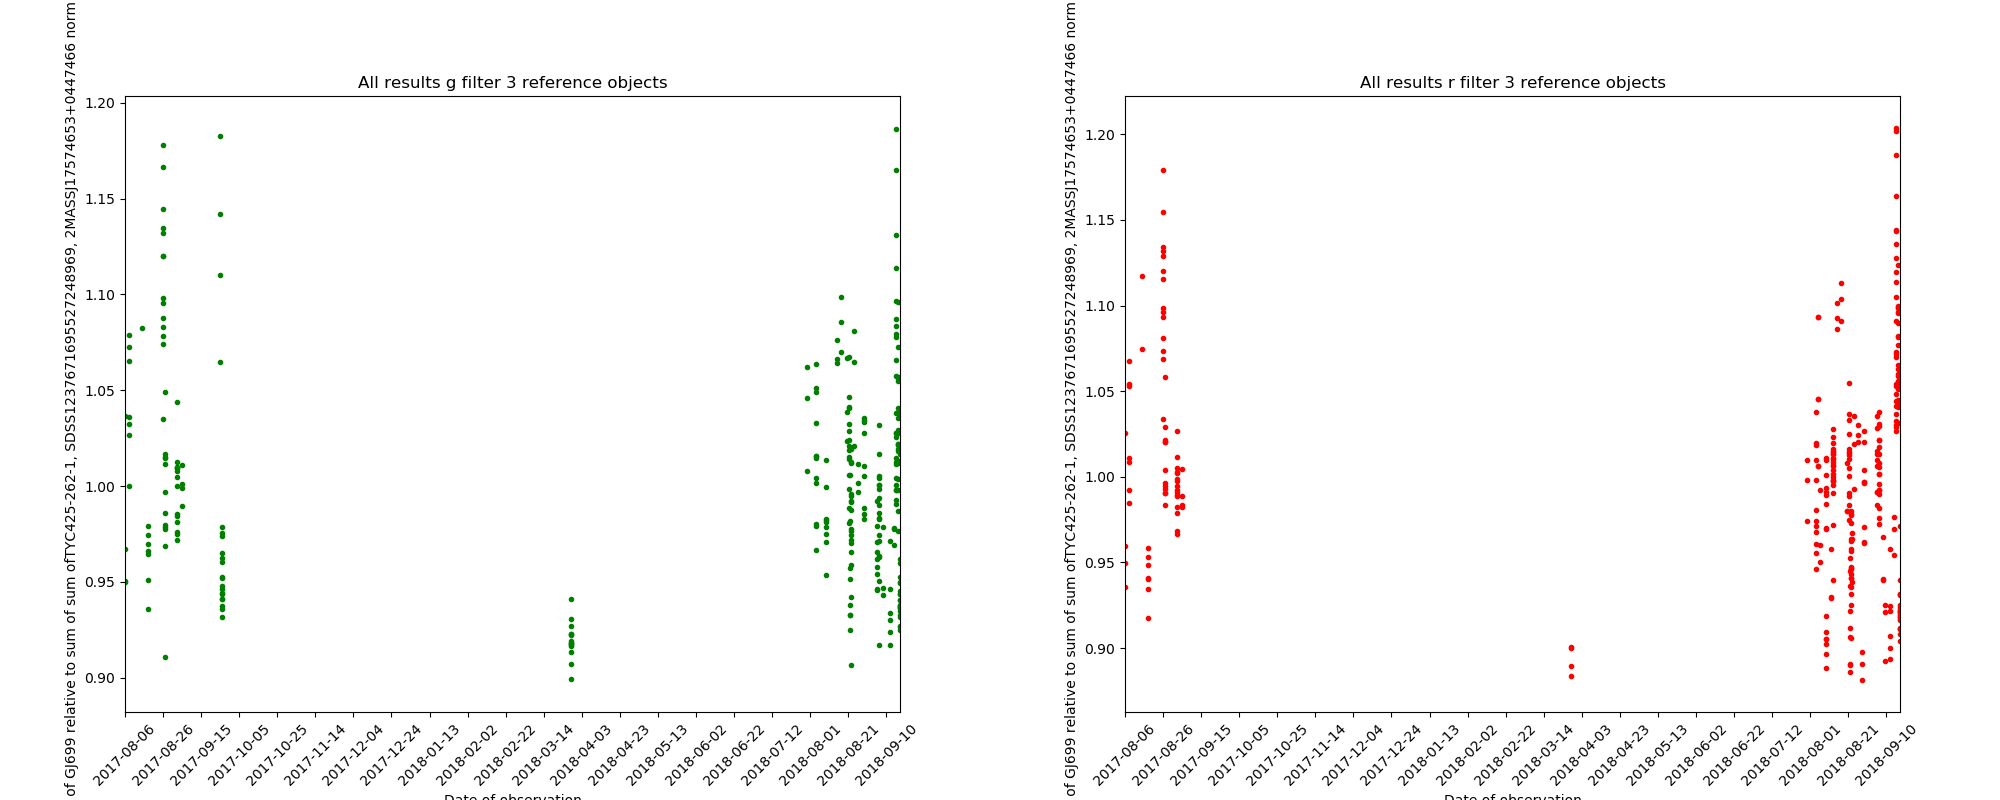
\includegraphics[scale=0.25]{images/allref123.png}
\end{center}   
\caption{This shows the ratio of the flux for the target, \bstar, to the 3 main reference objects for the \textbf{g} and
\textbf{r} filters, plotted as green and red respectively.}
  \protect\label{fig:allref123}
\end{figure}

\begin{figure}[!htbp]
\begin{center}
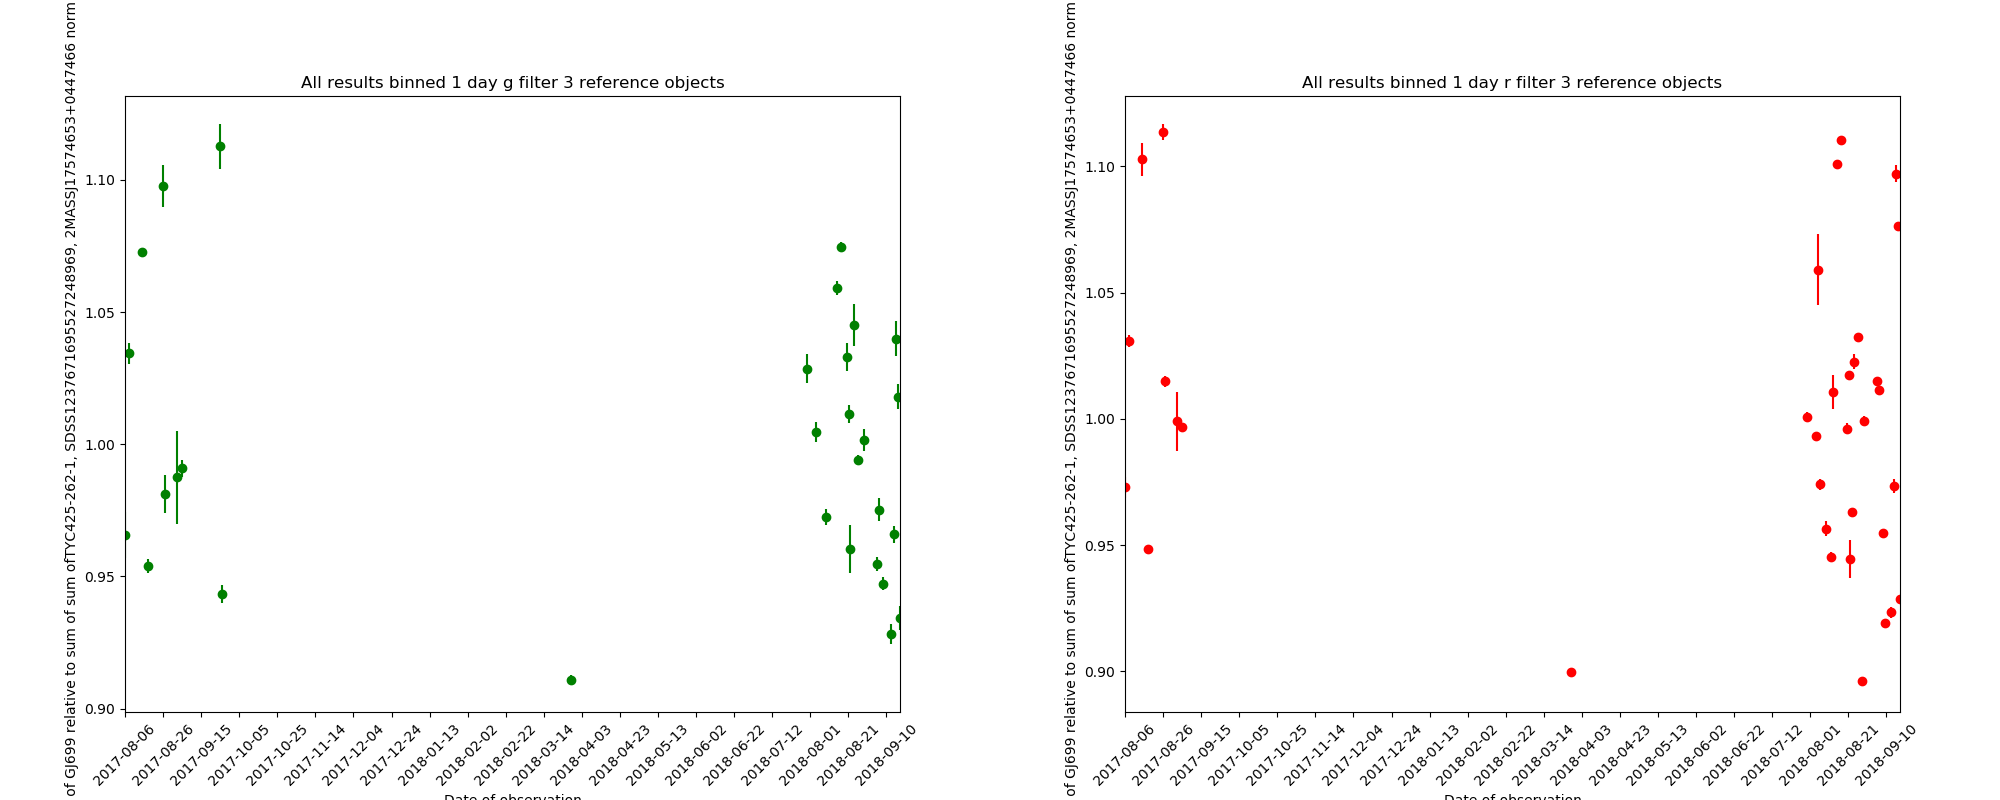
\includegraphics[scale=0.25]{images/allref123bin.png}
\end{center}   
\caption{This shows the ratio of the flux for the target, \bstar, to the 3 main reference objects as per Fig. \ref{fig:allref123} and binned to 1 day.}
  \protect\label{fig:allref123bin}
\end{figure}

\begin{figure}[!htbp]
\begin{center}
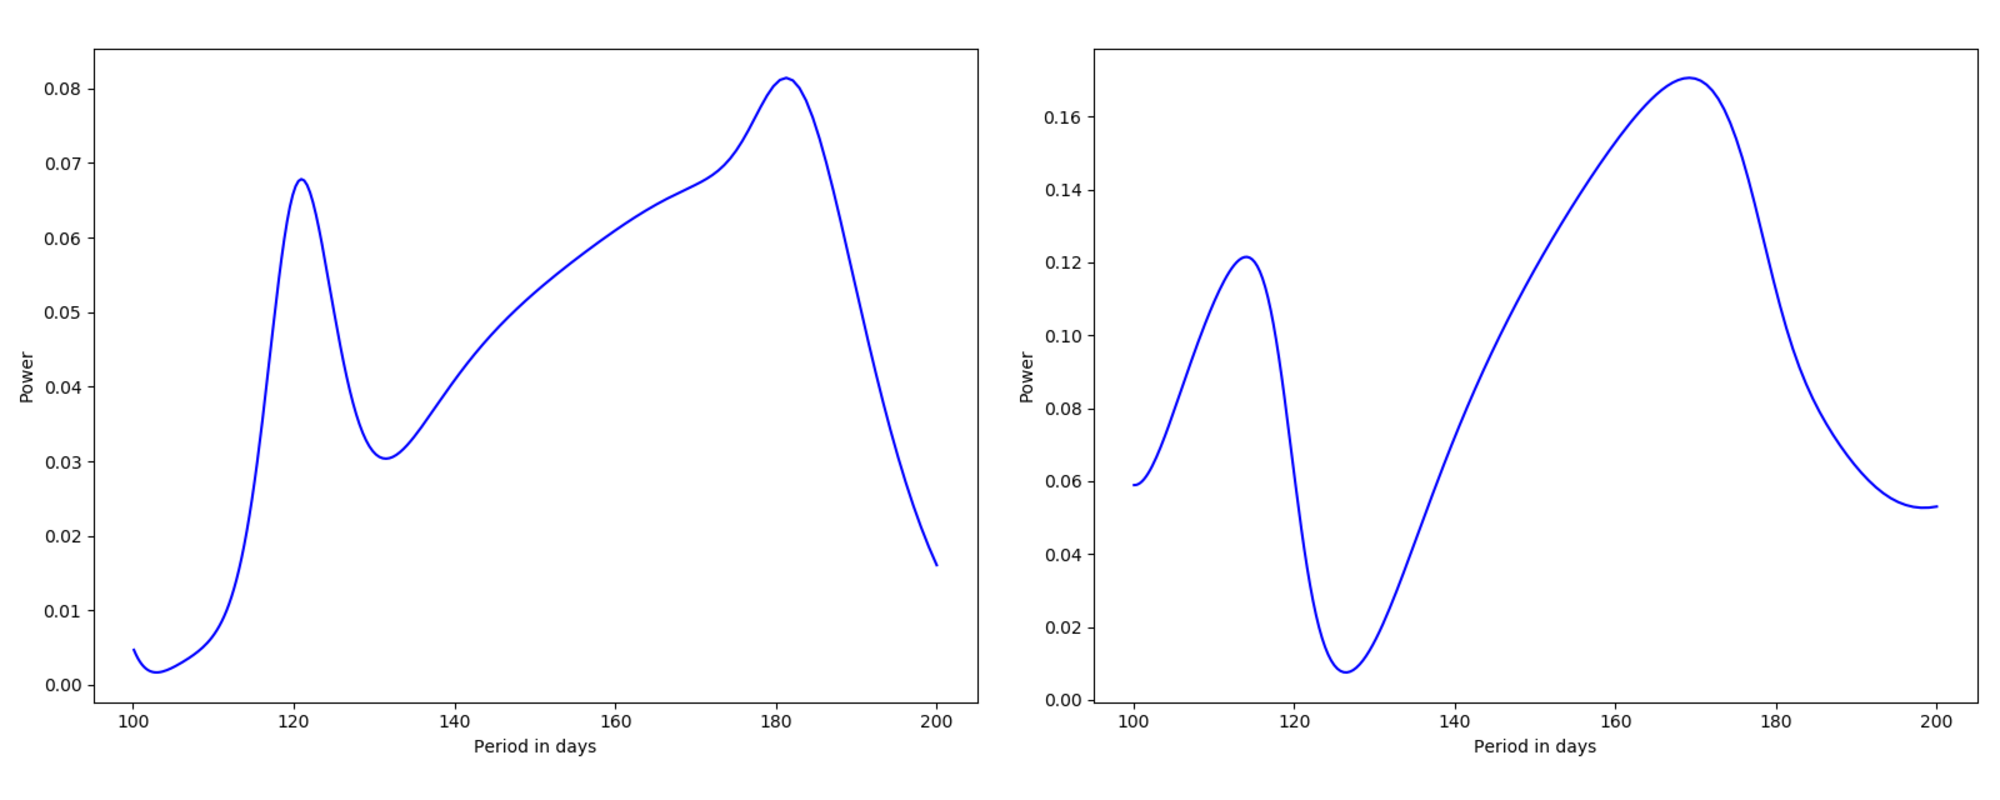
\includegraphics[scale=0.25]{images/ls123both.png}
\end{center}   
\caption{Periodograms obtained from Fig. \ref{fig:allref123}, left panel and Fig. \ref{fig:allref123bin} in right
  panel. Only the \textbf{g} filter was used in this plot, the one from the \textbf{r} filter being almost identical.}
  \protect\label{fig:ls123both}
\end{figure}

\begin{figure}[!htbp]
\begin{center}
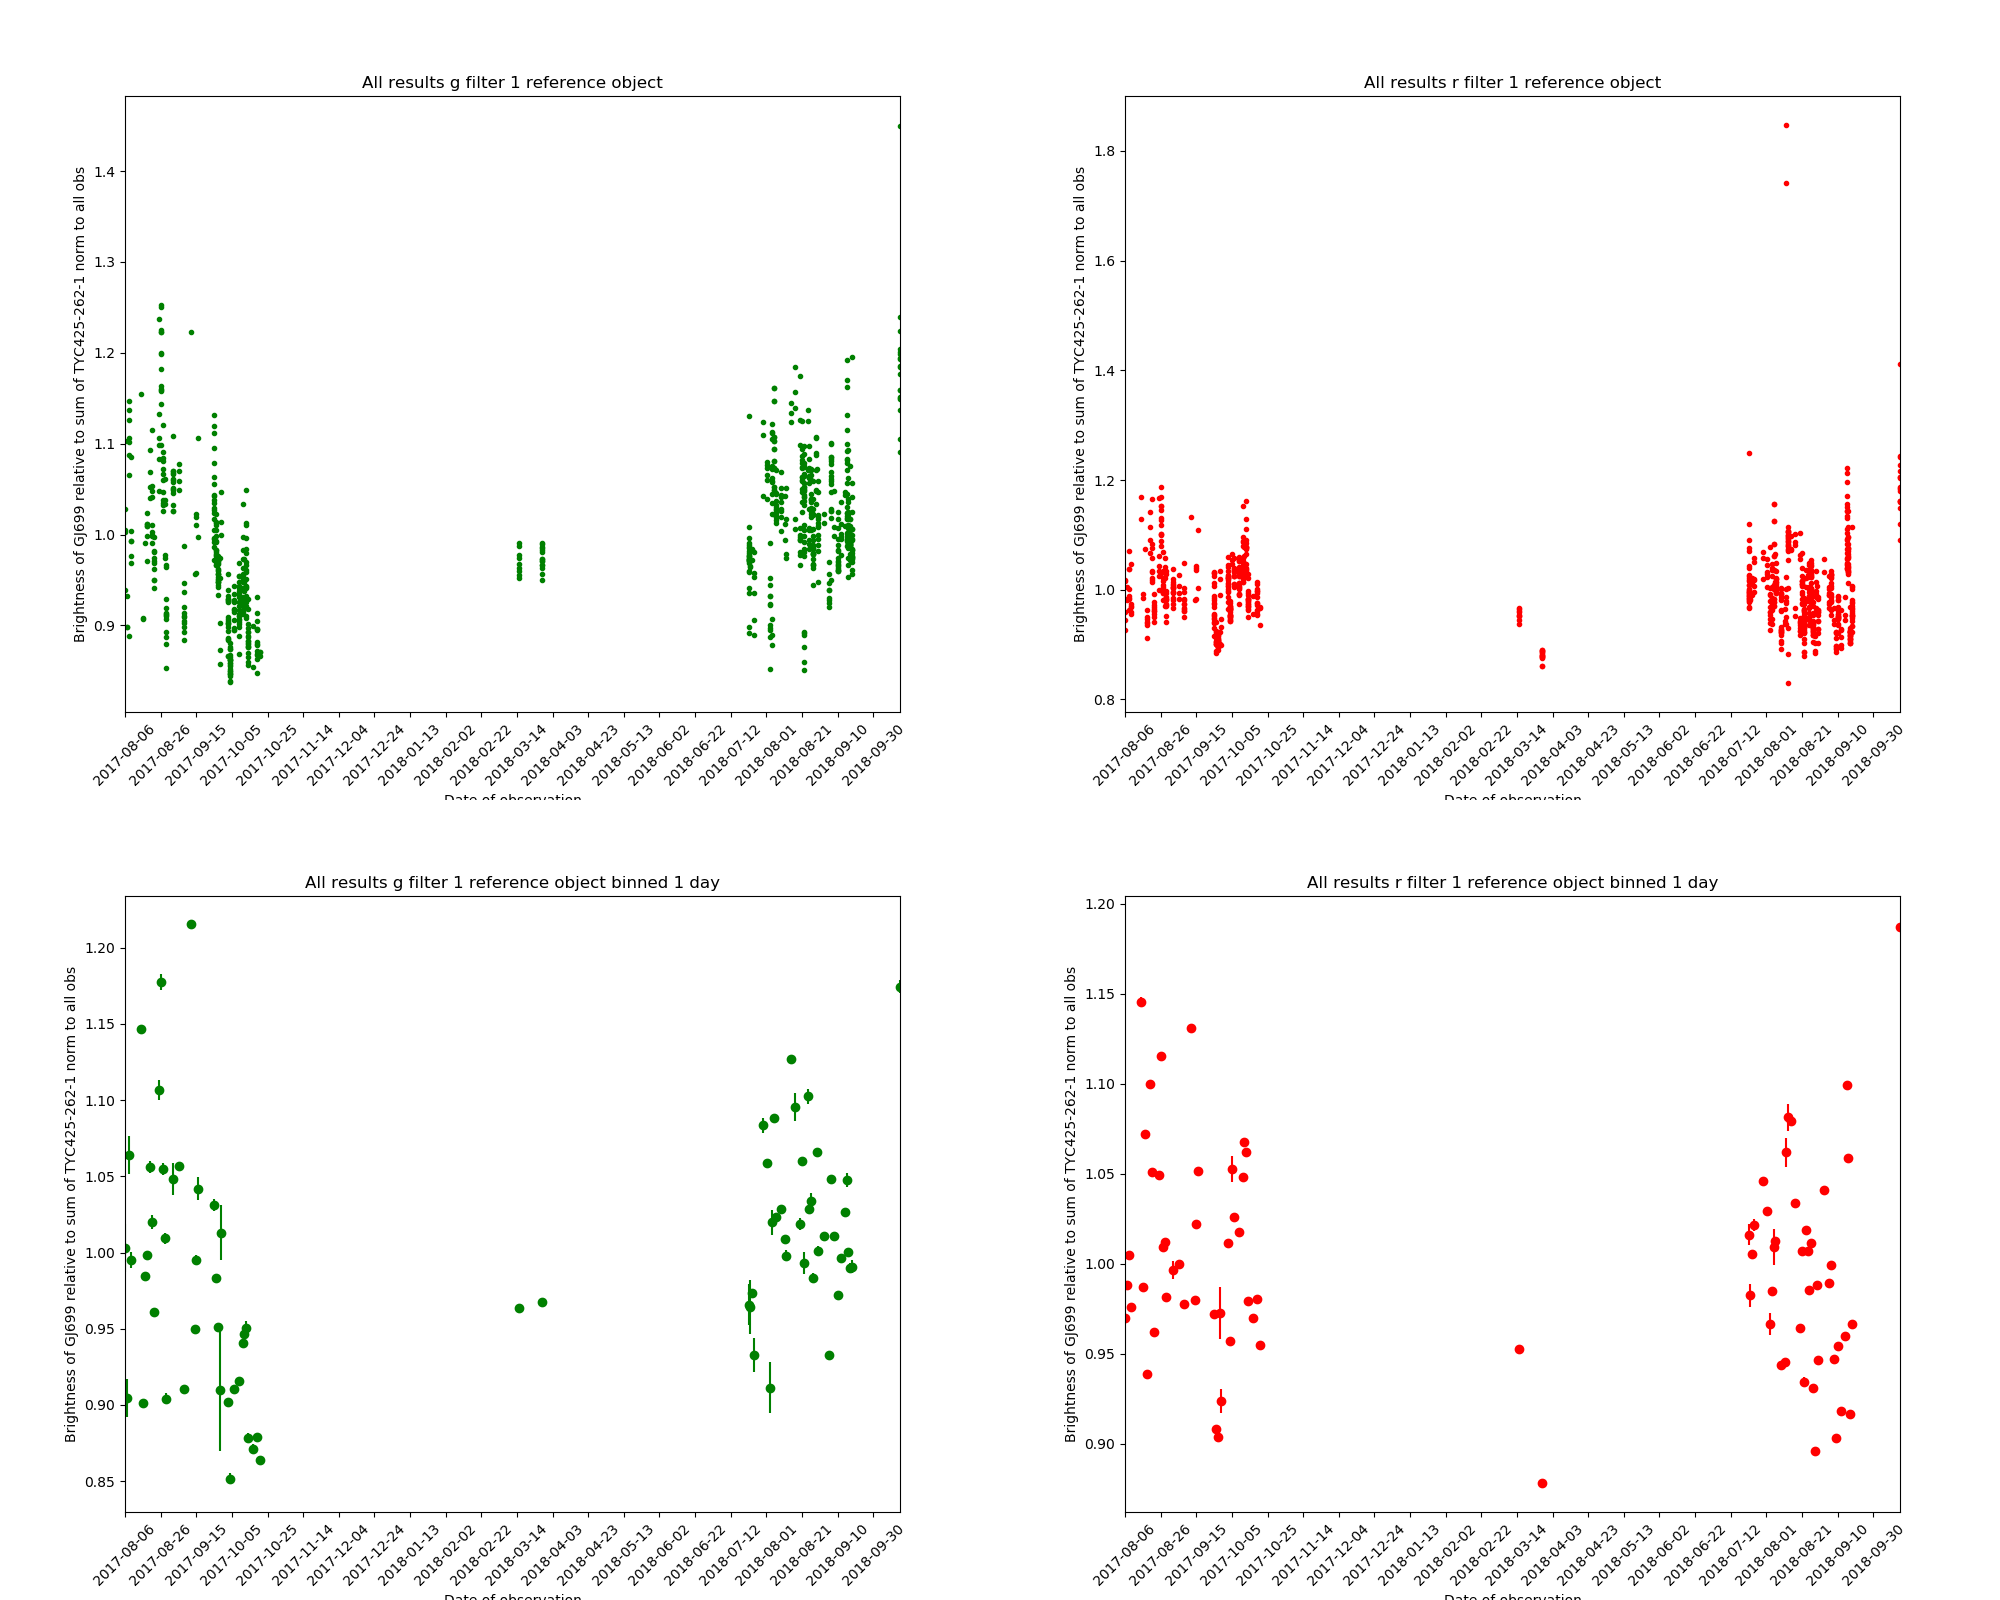
\includegraphics[scale=0.25]{images/allref1.png}
\end{center}   
\caption{This shows the ratio of the flux for the target, \bstar, to the strongest of the reference objects, TYC425-262-1.}
  \protect\label{fig:allref1}
\end{figure}

\begin{figure}[!htbp]
\begin{center}
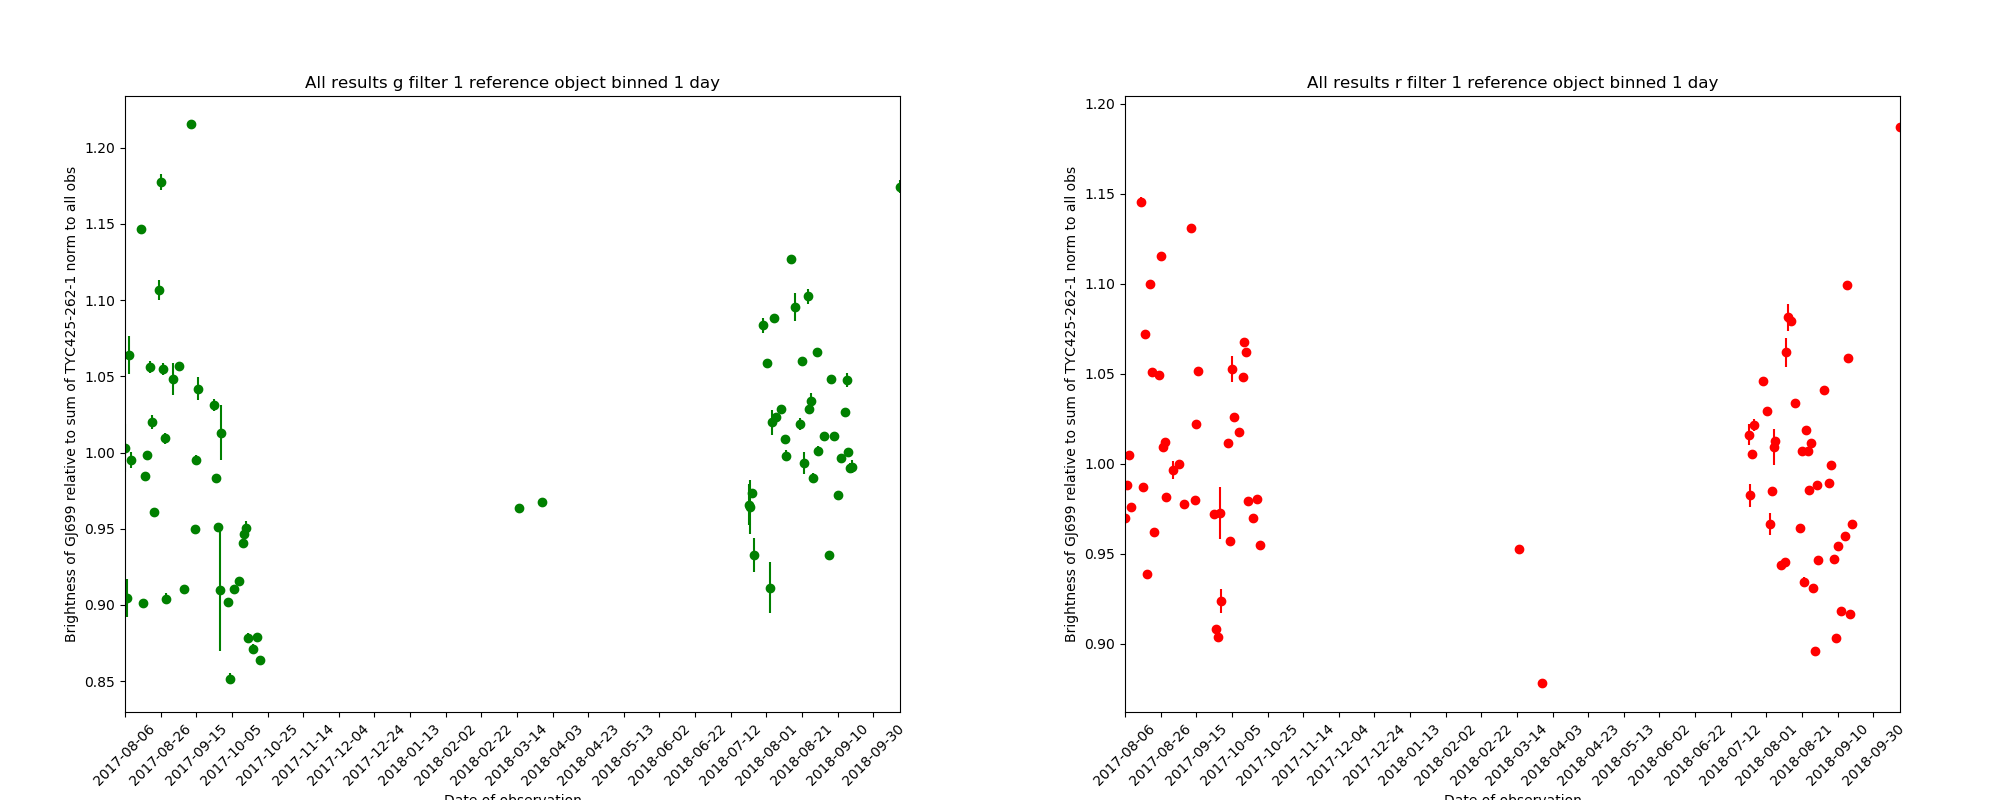
\includegraphics[scale=0.25]{images/allref1bin.png}
\end{center}   
\caption{This shows the ratio of the flux for the target, \bstar, to the strongest of the reference objects,
  TYC425-262-1 per Fig. \ref{fig:allref1} and binned to 1 day.}
  \protect\label{fig:allref1bin}
\end{figure}

\begin{figure}[!htbp]
\begin{center}
\includegraphics[scale=0.25]{images/ls1both.png}
\end{center}   
\caption{Periodograms obtained from Fig. \ref{fig:allref1}, left panel and Fig. \ref{fig:allref1bin} in right
  panel. Only the \textbf{g} filter was used in this plot, the one from the \textbf{r} filter being almost identical.}
\protect\label{fig:ls1both}
\end{figure}
\clearpage

\section{Further work}
\protect\label{section:worktocome}

The following is the programme of work I need to undertake to ready the project
to a state where serious science can be achieved.

In all cases, the work to be done will need revisiting and refining and
``iterating until convergence'' achieved.

\subsection{Completion and improvement of work to date}
\protect\label{section:fwimprovecompletion}

This currently documents work in progress and the following needs to be achieved
or at least an initial version complete before the project is ready to move
forward.

\subsubsection{Completion of revised calibration}
\protect\label{section:fwcalib}

I need to put together the work on revised bias and flat files, also of bad
pixel identification, so as to minimise the loss of useful data, refining whether
to discard a pixel altogether or assign a low weighting.

Some parts, especially of limits to flat fields, may not be needed; there is
plenty of scope for refinement.

Also needed is a reasonable assessment of the uncertainty of any measurements
taken.

I need to insert new versions of Fig. \ref{fig:initgexample} and following
into this report in section \ref{section:postcalibration} showing improvements
made.in these fields, with a first version ready by the end of the first week in
June 2022.

\subsubsection{Revise identification of objects other than targets}
\protect\label{section:fwtargets}

I populated the database of objects from SIMBAD and GAIA EDR3 in May 2021 and
this needs revising. Some of the objects are closer to each other than the
resolution of the telescope, about 0.6 arc-seconds per pixel, can distinguish.

The identification of close objects is currently slightly random due to the
different orientations of the images and the order in which the search
algorithm takes sources. It may be that there are larger common subsets of
reference objects than are currently apparent. It may well be feasible to
regard close objects as a composite object for the purposes of using as
reference objects.

This will need doing with some care and I would hope to be confident of the
results for at least {\prox} by the end of June 2022.

\subsubsection{Optimise apertures and determine magnitudes and variability of
reference objects} \protect\label{section:fwoptap}

In order to evaluate magnitudes over all the images, it is necessary to have
confidence in the reference objects available in all of the images, rather than
the common subset of objects which appears in all images, which becomes
vanishingly small, especially for {\ross} and {\bstar} and for the \texttt{i}
and \texttt{z} filters.

This will need running through and comparing each object with each other object,
this is more of a processing issue than anything.

It would be desirable to build a picture of variability and compare this with the
variability statistics from other sources, so that an uncertainty figure can
be made for each target.

Also needed is a standard optimised aperture size for calculation of the
brightness of objects in any given image.

Although this is a highly iterative process, I should hope to have a ``first
pass" of this complete by mid-August 2022.

\subsection{Extraction of data}
\protect\label{section:fwextract}

The whole object is to obtain believable light curves and observational data
from the REM image data including values for uncertainty in which it is possible
to have confidence and this is what I intend to present by the end of September
2022.

Obtaining periodic data is particularly important and a clear objective of this
study would be to try to obtain this for \ross, (and consequently the
inclination angle) although as discussed in Section \ref{section:introross}. with a maximum
period of $3.5 \pm 1.5$ days, but with observation days months apart as shown in Fig. \ref{fig:rdwarfhist}, there will
be a considerable number of aliases to contend with.

Obviously too, an increase in the understanding of activity cycles of all three
main targets will hopefully be a useful consequence of this.

\subsection{Calculation of Barycentric dates, periodograms}
\protect\label{section:fwbarycentric}

Barcycentric dates need to be computed and inserted into the observation records
before periodograms can be extracted. Then need to start producing periodograms
of the data.

\subsection{Variations and improvements}
\protect\label{section:fwvariations}

There are a substantial number of choices made in the analysis of the data and
scope for seeing whether improvements in the accuracy can be brought about by
tuning some of them. In mind are:

\begin{enumerate}
  \item Using a weighted sum in calculating peaks as opposed to summing the ADUs
  and calculating the error.
  \item Using sub-standard images with weightings.
  \item Experiment with weightings of areas round the edges of the images, where
  vignetting and other effects affect the exposures.
  \item Using different sized apertures with different filters.
  \item Selection of different reference objects with different filters.
  \item Asking for changes to the exposure times.
  \item Plotting of periods of other objects found in the frames.\footnote{It
  might be necessary to revise the Barycentric dates in these cases but the
  ones for the targets will probably be accurate enough, but must check.}
\end{enumerate}

\subsection{Incorporation of other data}
\protect\label{section:fwincorp}

There is a complete set of REMIR data taken simultaneously with all the other
options, with calibration already done. It would be wasteful not to make
maximums use of this for comparison and for incorporation into the results where
possible.

Reference object sets are a little more limited with these as the {\rdwarf}
targets are so much brighter in the Infrared compared to the others.

I also intend to look at other datasets and where possible undertake a similar
task with these.

\clearpage

\appendix 
\section{Database and interfaces}
\protect\label{section:database}

In order, to facilitate the analysis of the data, I created a database
constructed to be able to retrieve given observations or other data according to
criteria as required, together with a set of Python interfaces, using
\textit{Numpy} and other facilities including routines from \textit{Astropy}.

The tables in this database are as follows.

\begin{description}
\item[obsinf] Information about observations.
\item[iforbinf] Information about individual flat and bias files.
\item[forbinf] Information about master flat and bias files.
\item[objdata] Details of objects in the vicinity of target objects.
\item[objalias] Alternative names for objects in \textbf[objdata].
\item[objpm] Records of positions of objects with appreciable proper motions.
\item[findresult] Notes of objects found in each observation.
\item[fitsfile] Copies of the FITS files for observations in active
consideration.
\end{description}

Not all of the FITS files are stored; only those with the visible light filters
and of the target {\rdwarf} objects are saved. The Python routines are designed
to transparently either fetch a FITS file from the database \textbf[fitsfile]
table or fetch from the Red Dots project database (with optional local
caching) as required.

\subsection{The obsinf table}
\protect\label{section:obsinftable}

The \textbf{obsinf} table records details of observations taken from the
relevant FITS file (which may be saved locally in the \textbf{fitsfile} table).

Columns in this database give the following information, and a Python routine
enables a selection of records of observations to be retrieved according to
ranges of these criteria.

\begin{description}
\item[obsind] A unique integer used for internal cross-reference.
\item[serial] The serial number of the observation at the Red Dots project.
\item[date\_obs] The date and time of the observation.
\item[object] The target object name
\item[filter] The filter.
\item[median] Median pixel value.
\item[mean] Mean pixel value.
\item[minv] Minimum pixel value.
\item[maxv] Maximum pixel value.
\item[std] Standard deviation of pixel value.
\item[skew] Skewness of pixel value.
\item[kurt] Kurtosis of pixel value.\footnote{Skewness and kurtosis are only
recorded as these are used in construction of the master flat files and this is
included for consistency with \textbf{iforbinf}.}
\item[moonphase] Phase of moon as percentage.
\item[moondist] Angular distance of moon from target.
\item[airmass] Airmass to target,
\item[quality] Quality assessment of observation, between 0 (rejected) and 1
(best).
\item[exptime] Exposure time.
\end{description}

\subsection{The iforbinf table}
\protect\label{section:iforbinftable}

The \textbf{iforbinf} table records details of individual flat or bias files
taken from the relevant FITS file (which may be saved locally in the \textbf{fitsfile} table).

Columns in this database give the following information, and a Python routine
enables a selection of records of the file to be retrieved according to
ranges of these criteria.

\begin{description}
\item[iforbind] A unique integer used for internal cross-reference.
\item[typ] Type of file, \texttt{flat}, \texttt{bias} or \texttt{dark}.
\item[serial] The serial number of the file at the Red Dots project.
\item[date\_obs] The date and time for taking the file.
\item[filter] The filter (only \texttt{g}, \texttt{i}, \texttt{r} or
\texttt{z}).
\item[median] Median pixel value.
\item[mean] Mean pixel value.
\item[minv] Minimum pixel value.
\item[maxv] Maximum pixel value.
\item[std] Standard deviation of pixel value.
\item[skew] Skewness of pixel value.
\item[kurt] Kurtosis of pixel value.\footnote{Skewness and kurtosis are only
recorded as these are used in construction of the master flat files.}
\end{description}

\subsection{The objdata table}
\protect\label{section:objdatatable}

The \textbf{objdata} table records details of objects in the vicinity of one of
the target objects).

Columns in this database give the following information, and a Python routine
enables objects in the vicinity of a given target to be retrieved, making
appropriate allowances for proper motions (in conjunction with the
\textbf[objpms] table).

\begin{description}
\item[ind] A unique integer used for internal cross-reference.
\item[objname] An internal name for the object (short names such as
\textbf{GJ551} for {\prox} are preferred).
\item[dispname] A name to be used for displays. Latex format is used for easy
insertion of results into Latex reports such as this, for example {\prox} is
stored as \texttt{$\backslash$prox}.
\item[objtype] Type of object, such as \texttt{Star}.
\item[radeg] \texttt{J2000}-based Right Ascension in degrees.
\item[decdeg]\texttt{J2000}-based Declination in degrees.
\item[rapm] Proper motion in Right Ascension, in milli-arcseconds / year.
\item[decpm]Proper motion in Declination, in milli-arcseconds / year.
\item[apsize]Optimised aperture size, possibly fractional.
\end{description}

This is combined with various brightness information, in various bands, together
with standard deviations. (These fields are currently not finalised).

\clearpage


\bibliographystyle{apj}
\bibpunct{(}{)}{;}{s}{,}{,}
\bibliography{bibrefs}

\protect\label{lastpage}
\end{document}
